\documentclass[12pt ]{book}
%\documentclass[10pt,a5paper]{book}
\usepackage[utf8]{inputenc}
\usepackage{amsmath,amsfonts,amssymb,euscript,dcolumn}
%\usepackage[english,russian,french,hebrew,]{babel}
%\usepackage[english,hebrew]{babel}
\usepackage[english,french ]{babel}
\usepackage{graphicx}
\usepackage{caption}
%\textwidth  109mm%109mm  % 170mm
%\textheight 162mm%240mm  %240/12
%\hsize=  170truemm
%\topmargin -16mm
%\oddsidemargin 1.3cm % this for the A5 printer
%\evensidemargin -0.4cm
% this for the A5 printer

\textwidth    170mm    %A4
\textheight   240mm    %A4
%\hsize=  170truemm
\topmargin -16mm
%\oddsidemargin -1.8cm % this for the A5 printer
%\evensidemargin -1.8cm
% this for the A5 printer
\oddsidemargin -0.4cm % this for the A5 printer
\evensidemargin -0.4cm

%\DeclareUnicodeCharacter{2055}{\runTask}
%\DeclareRobustCommand\runTask{%
%  \unskip\nobreak\thinspace\textemdash\allowbreak\thinspace\ignorespaces}
%\renewcommand{\contentsname}{Оглавление}\contentsname
\makeatletter
%\newcommand{\l@abcd}[2]{\hbox to \textwidth{#1 {\huge\dotfill} #2}}
%\newcommand{\l@Myabcd}[2]{\hbox to \textwidth{ #1 \leaders\hbox{~ }\hfil  }}
%%%%%%%%%%%%%%%%%%%%%%%%%%%%%%%%%%%%%%%%%%%%%%%%%%%%%%%%%%%%%%%%%%%%%%%%%%
\renewcommand{\l@chapter}[2] %Начало макроопределения (***глава в оглавлении***)
{\pagebreak[3] \vspace{1em plus 1pt}%
  \@tempdima=4.5em% место для номера главы (1.5em в стандарте)
  %\@pnumwidth=2em
    {% Дальше внутри группы...
   \rightskip=\@pnumwidth
   \leftskip=\@tempdima
   \bf
   \noindent
   \hspace{-\leftskip}% с левого поля
    #1 %\nolinebreak
   %\leaders\hbox to 0.5em {\hss. \hss }
\hfill
%\nolinebreak
    \rlap{\makebox[\@pnumwidth][r]{#2}}\par
    \nopagebreak[3]
   } %конец группы.
}% конец макроопределения

%%%%%%%%%%%%%%%%%%%%%%%%%%%%%%%%%%%%%%%%%%%%%%%%%%%%%%%%%%%%%%%%%%%%%%%%%%%%
\renewcommand{\@makechapterhead}[1]{ %Начало макроопределения (***для главы***)
 \vspace*{40pt} %Пустое место вверху страницы
 {\parindent=0pt
  \raggedright\Large\bf
  %\@chapapp{} %\@chapapp печатает слово"Глава"(см. ниже)
 {\Huge \bf Chapter \arabic{chapter} }   %  \par  % чтобы номер главы - в отдельной строке
  \vspace{20pt} % между словом "Глава"и её заголовком
 \par
\Huge \bf #1
%\begin{centerline} #1  \end{centerline}   \centerline
%#1
\par % заголовок главы
  \nopagebreak %чтоб не оторвать заголовок от текста
  \vspace{40pt} % между заголовком и текстом
 } %конец группы.
}% конец макроопределения
%%%%%%%%%%%%%%%%%%%%%%%%%%%%%%%%%%%%%%%%%%%%%%%%%%%%%%%%%%%%%%%%%%%%%%%%%%
\renewcommand{\section}{\@startsection{section} %(***для раздела***)
 {1} %уровень вложенности раздела
 {0mm} %отступ от левого поля
 {3.5ex plus 1ex minus 2.ex } %вертикальный отступ До
 {2.3ex plus 0.2ex } %вертикальный отступ После
 {  \Large \bfseries
%\centerline
}% стиль
}% конец
%%%%%%%%%%%%%%%%%%%%%%%%%%%%%%%%%%%%%%%%%%%%%%%%%%%%%%%%%%%%%%%%%%%%%%%%%%
\def\Nthechapter{\arabic{chapter}}
\renewcommand{\@begintheorem}[2]{\begin{trivlist}\it
             \item[\hspace{\labelsep}{\bf #1\ #2.}]}
\renewcommand{\@biblabel}[1]{#1.\hfill}
%\renewcommand{\thechapter}{{\bf {Глава} \arabic{chapter}.   }}
\renewcommand{\thechapter}{{\arabic{chapter}}}
\renewcommand{\thesection}{\arabic{chapter}.\arabic{section}.}
\renewcommand{\thesubsection}{\arabic{chapter}.\arabic{section}.\arabic{subsection}.}
\renewcommand{\thesubsubsection}
             {\arabic{chapter}.\arabic{section}.\arabic{subsection}.\arabic{section}.}
%%%%%%%%%%%%%%%%%%%%%%%%%%%%%%%%%%%%%%%%%%%%%%%%%%%%%%%%%%%%%%%%%%%%%%%%%%%%%%%%%
%\renewcommand{\subsection}{\@startsection{subsection} %(***для подраздела***)
% {1} %уровень вложенности раздела
% {0mm} %отступ от левого поля
% {3.5ex plus 1ex minus 2.ex } %вертикальный отступ До
% {2.3ex plus 0.2ex } %вертикальный отступ После
% {  \large \bfseries   }% стиль
%}% конец
%%%%%%%%%%%%%%%%%%%%%%%%%%%%%%%%%%%%%%%%%%%%%%%%%%%%%%%%%%%%%%%%%%%%%%%%%%%%%%%%%
%\renewcommand{\subsubsection}{\@startsection{subsubsection} %(***для подподраздела***)
% {1} %уровень вложенности раздела
% {0mm} %отступ от левого поля
% {3.5ex plus 1ex minus 2.ex } %вертикальный отступ До
% {2.3ex plus 0.2ex } %вертикальный отступ После
% {  \bfseries   }% стиль
%}% конец

%\renewcommand{\@begintheorem}[2]{\begin{trivlist}\it
%             \item[\hspace{\labelsep}{\bf #1\ #2.}]}
%\newtheorem {lemma} {\bf Лемма}
%\newtheorem {theorem} {\bf Теорема}
%\newtheorem {corollary} {\bf Следствие}
%\newtheorem {proposal} {\bf Предложение}
%\newtheorem {definition} {\bf Определение}


\makeatother

\newcounter{ctheorem}[chapter]
\newcounter{clemma}[chapter]
\newcounter{cproposal}[chapter]
\newcounter{cdefinition}[chapter]
\newcounter{ccorollary}[chapter]

% \def\theorem{\par \smallskip %\noindent
%      \refstepcounter{ctheorem}
%     {\bf  Теорема \arabic{chapter}.\arabic{ctheorem}.\ } \begin{it} }
% \def\lemma{\par\smallskip %\noindent
%      \refstepcounter{clemma}
%     {\bf  Лемма \arabic{chapter}.\arabic{clemma}.\ } \begin{it} }
% \def\proposal{\par\smallskip %\noindent
%      \refstepcounter{cproposal}
%     {\bf  Предложение \arabic{chapter}.\arabic{cproposal}.\ } \begin{it} }
% \def\definition{\par\smallskip %\noindent
%     \refstepcounter{cdefinition}
%     {\bf  Определение \arabic{chapter}.\arabic{cdefinition}.\ } \begin{it} }
% \def\corollary{\par\smallskip %\noindent
%     \refstepcounter{ccorollary}
%     {\bf  Следствие \arabic{chapter}.\arabic{ccorollary}.\ } \begin{it} }

\def\endtheorem{\end{it}\par\smallskip}
\def\endlemma{\end{it}\par\smallskip}
\def\endproposal{\end{it}\par\smallskip}
\def\enddefinition{\end{it}\par\smallskip}
\def\endcorollary{\end{it}\par\smallskip}

\newcommand{\ex}[2]{Returns: \\ in: #1 \\ out: #2 }
\newcommand{\comm}[2]{$\backslash {\mathbf {#1}} #2$}

\begin{document}

\sloppy
%\captionsetup[figure]{name=Figure}



\renewcommand{\theequation}{\arabic{chapter}.\arabic{equation}}

% %счетчик для примеров
% \newcounter{examplec}
% \setcounter{examplec}{0}
% \newcommand{\example}[1]{\addtocounter{examplec}{1}\null\underline{\textbf{Пример \arabic{examplec}}. #1} }
%
%
% \newcounter{tablec}
% \setcounter{tablec}{0}
% \newcommand{\mytable}[1]{\addtocounter{tablec}{1}{\begin{flushright}Таблица \arabic{tablec}\end{flushright}}\textbf{ #1}}


%\hsize=  170truemm
\def\refname{{\centerline{\Large{REFERENCES}}}}%
%\def\bibname{{\centerline{\normalsize{ЛИТЕРАТУРА}}}}%
\def\bibname{{\centerline{\Large{REFERENCES}}}}%
\def\abstractname{{{ \  }}}%Аннотация
\def\chaptername{ \hspace{200pt} \Large Chapter}%
%\def\appendixname{Приложение}%
\def\contentsname{\centerline{\Large{CONTENTS}}}%
% \def\listfigurename{Список рисунков}%
% \def\listtablename{Список таблиц}%
% \def\indexname{Индекс}%
% \def\figurename{Рисунок}%
% \def\tablename{Таблица}%
% \def\partname{Часть}%
% \def\enclname{прилагается}%
% \def\ccname{копии}%
% \def\headtoname{Кому}%
% \def\pagename{Стр.}
\pagestyle{plain}



\newcommand{\diag}{{\mathrm{diag}}}
\newcommand{\sign}{{\mathrm{sign}}}
\newcommand{\Nr}{\,{\mathrm{Nr}}\,}
\newcommand{\rank}{{\mathrm{rank}}}
\newcommand{\ce}{\centerline}
\newcommand{\e}{{\mathbf e}}
\newcommand{\tb}{ \tilde{b}}
\newcommand{\tB}{ \tilde{B}}
\newcommand{\tD}{ \tilde{D}}
\newcommand{\tA}{ \tilde{A}}
\newcommand{\tF}{ \tilde{F}}
\newcommand{\tx}{ \tilde{x}}
\newcommand{\hbx}{{\hat{\mathbf x}}}
\newcommand{\bx}{{\mathbf x}}
\newcommand{\bZ}{{\mathbb Z}}

\def\head#1{\vskip6pt{\bf #1}}
\newcommand{\intt}{{\bf int }}

\newcommand{\ra}{\rangle}
\newcommand{\la}{\langle}
\newcommand{\ul}{\Large \bf  \underline }
\newcommand{\tchi}{{\tilde{\mathbf \chi}}}
\newcommand{\mtr}[4]%
{\left(\begin{array}{cc}#1 & #2\\#3 & #4\end{array}\right)}
\newcommand{\Dmtr}[4]%
{\left|\begin{array}{rr}#1 & #2\\#3 & #4\end{array}\right|}

\newcommand{\mtrk}[4]%
{\left[\begin{array}{cc}#1 & #2\\#3 & #4\end{array}\right]}

\newcommand{\mtrc}[2]%
{\left(\begin{array}{c}#1 \\#2 \end{array}\right)}
\newcommand{\mtrs}[2]%
{\left[\begin{array}{c}#1 \\#2 \end{array}\right]}
 \newcommand{\LCM}{{\mathrm{LCM}}}
% \newcommand{\R}{{\bf R}}
\date {}
\newcommand{\tsec}[1]{\bigskip \centerline{\normalsize {#1}}\bigskip \par}
\newcommand{\ttsec}[2]{\bigskip {\centerline{\normalsize {#1}}}\par\noindent
{\centerline{\normalsize {#2}}} \bigskip}
\newcommand{\tttsec}[3]{\bigskip {\centerline{\normalsize {#1}}}
\par\noindent
{\centerline{\normalsize {#2}}} \par\noindent
{\centerline{\normalsize {#3}}} \bigskip}
\newcommand{\tsub}[1]{{\medskip \bf {#1}}\par}


%\pageno=1
%\magnification \magstep2

% Я \hoffset=30truemm
% Я \voffset=20truemm
\frenchspacing
%\NoRunningHeads
%\TagsOnRight
%\LimitsOnInts
%\LimitsOnSums
%\widowpenalty=150 % было 10000
%\clubpenalty=150  % было 10000
%\binoppenalty=150
%\relpenalty=150



\def\endd{\vfill\eject}
\def\Beta{\roman B}

\let\eps\varepsilon
\def\const{\operatorname{const}}
\def\R{{\Bbb R}}
\def\K{{\Bbb K}}
\def\N{{\Bbb N}}
\def\Z{{\Bbb Z}}
\def\al{\alpha}
\def\be{\beta}
\def\beF{\widehat{\bf \beta}}
\def\alF{\widehat{\bf \alpha}}
\def\de{\delta}
\def\deF{\widehat{\bf \delta}}
\def\si{\sigma}
\def\siF{\widehat{\bf \sigma}}
\def\di{{\bf {\rm diag}}}
\def\G{\Gamma}
\def\L{\Lambda}

\def\cA{{\bf \mathcal A}}
\def\cC{{\bf \mathcal C}}
\def\cD{{\bf \mathcal D}}
\def\cG{{\bf \mathcal G}}
\def\cH{{\bf \mathcal H}}
\def\cL{{\bf \mathcal L}}
\def\cK{{\bf \mathcal K}}
\def\cM{{\bf \mathcal M}}
\def\cT{{\bf \mathcal T}}
\def\cS{{\bf \mathcal S}}
\def\cU{{\bf \mathcal U}}
\def\cY{{\bf \mathcal Y}}
\def\cZ{{\bf \mathcal Z}}


\def\cAF{{\widehat {\bf \cal A}}}
\def\cGF{{\widehat {\bf \cal G}}}
\def\cFF{{\widehat {\bf \cal F}}}
\def\cHF{{\widehat {\bf \cal H}}}
\def\cLF{{\widehat {\bf \cal L}}}
\def\cMF{{\widehat {\bf \cal M}}}
\def\cVF{{\widehat {\bf \cal V}}}
\def\cUF{{\widehat {\bf \cal U}}}
\newcommand{\bR}{{\mathbf R}}
\newcommand{\bL}{{\mathbf L}}
\newcommand{\bM}{{\mathbf M}}
\newcommand{\bU}{{\mathbf U}}
\newcommand{\bA}{{\mathbf A}}
\newcommand{\bB}{{\mathbf B}}
\newcommand{\bC}{{\mathbf C}}
\newcommand{\bD}{{\mathbf D}}
\newcommand{\bF}{{\mathbf F}}
\newcommand{\bE}{{\mathbf E}}
\newcommand{\bG}{{\mathbf G}}
\newcommand{\bW}{{\mathbf W}}
\def\ba{{\mathbf a}}
\def\bp{{\mathbf p}}
\def\bq{{\mathbf q}}
\def\br{{\mathbf r}}
\def\bK{{\mathbf K}}
\def\leq{\leqslant }
\def\geq{\geqslant }
\def\tF{\widetilde{F}}
\def\tG{\widetilde{G}}
\def\tL{\widetilde{L}}
\def\tl{\widetilde{\ell}}
\def\tM{\widetilde{M}}
\def\tU{\widetilde{U}}
\def\tV{\widetilde{V}}
\def\tW{\widetilde{W}}
\def\tu{\widetilde{u}}
\def\btL{\widetilde{\mathbf {\rm L}}}
\def\btU{\widetilde{\mathbf {\rm U}}}
%_________________
\def\tcF{\widetilde{\cal F}}
\def\tcL{\widetilde{\cal L}}
\def\tcM{\widetilde{\cal M}}
\def\tcU{\widetilde{\cal U}}
\def\Ann{\rm {Ann \,}}
\def\GI{\rm {GI \,}}
\def\Frac{\rm {Frac \,}}
\def\GCD{\rm {НОД \,}}

 \renewcommand{\figurename}{Figure }

\thispagestyle{empty}


\begin{LARGE}
\bf{
\centerline{ Language Guide}
\centerline{}
\centerline{}

\centerline{`` MATHPAR ''}
}
\end{LARGE}
\centerline{}
\centerline{}
\centerline{}
\centerline{}
 \centerline{VERSION 6.00 }
\vfill

\ce{  10.02.2016  }
%--------------------------------------------------------------------------------
\tableofcontents
\vfill
\eject

\chapter{Введение}
Данное руководство по языку Mathpar поможет Вам при решении математических задач. 
Оно будет всегда Вашим помощником, когда Вам нужно воспользоваться математикой:
будь то решение задачи в школе или в университете, выполнение научных расчетов или решение производственной задачи.

Mathpar поможет Вам делать простые числовые или алгебраические операции, строить графики кривых и поверхностей.

Он поможет Вам решать задачи различных разделов математического анализа, алгебры, геометрии, задачи по физике, по химии и другие.  

Если же Вы профессионально применяете математику, то он поможет Вам избавиться от рутинных вычислений и оперировать с очень большими математическими объектами, задействуя при этом суперкомпьютеры. 
Mathpar позволяет оперировать с функциями и функциональными матрицами, получать как точные численно-аналитические решения, так и решения, в которых числовые коэффициенты получаются с требуемой степень точности.

В основе языка Mathpar лежит широко используемый математиками  и физиками язык ТеХ, который обычно используют для набора математических текстов.

Вы можете сохранить как постановку задачи, так и ход ее решения. При этом можете сохранять и текстовый вид (Mathpar, TeX или MathML) и изображение (pdf, jpg).

Весь излагаемый тут материал делится на 14 глав.

Для первого знакомства достаточно ознакомиться с двумя следующими главами данного руководства. 

Во второй главе описывается ввод данных и выполнение простейших вычислений. 
Даются обозначения для элементарных функций, таких как логарифм, синус, косинус и т.д., 
и констант --- $\pi$, $e$, $i$, а также констант, которые необходимы для задания числовых множеств. 
Описываются способы задания векторов и матриц, арифметические операции над ними, команды генерации случайных чисел, полиномов и матриц, команды для решения алгебраических уравнений. 
Для всех команд приведены примеры.

Третья глава посвящена построению графиков функций. Mathpar позволяет строить графики функций, которые заданны явно или параметрически,
кроме того функции могут быть заданы таблично -- множеством значений функций на конечном множестве значений аргумента. 
Можно выполнить построение нескольких графиков в одной системе координат. 

В четвертой главе описываются способы задания окружения в системе Mathpar, т.е. того пространства, 
в котором будут определяться математические объекты. 
В любой момент Вы можете сменить окружение и задать новое алгебраическое пространство.  

В пятой главе описаны команды для задания математических функций одной или нескольких переменных, их композиций, вычисления значений функции в точке, подстановки выражений в функции, вычисление предела функции в точке, символьного интегрирования композиций элементарных функций. Приводятся примеры выполнения   команд. 

Шестая глава посвящена действиям с рядами. Рассматриваются способы задания ряда. Даются команды для сложения, вычитания, умножения двух рядов и для разложения функции в ряд Тейлора с определенным количеством членов ряда. 

В седьмой главе описаны команды для решения обыкновенных дифференциальных уравнений и систем, а также   дифференциальных уравнений с частными производными.

Восьмая глава посвящена полиномиальным вычислениям. Рассматриваются команды для вычисления значения полинома в точке, суммирования полинома по переменным, вычисления базиса Гребнера полиномиального идеала над рациональными числами. 

В девятой главе описываются матричные функции --- вычисление транспонированной матрицы, определителя матрицы, присоединенной и обратной матриц, эшелонной формы матрицы, ядра оператора, характеристического полинома матрицы и другие.

Десятая глава посвящена функциям теории вероятностей и математической статистики. Описывается задание дискретной случайной величины,  команды для вычисления математического ожидания дискретной случайной величины, дисперсии, среднего квадратичного отклонения, суммы, произведения двух дискретных случайных величин, коэффициента ковариации, коэффициента корреляции, построения многоугольника распределения и функции распределения дискретной случайной величины. В этой главе рассматриваются команды для задания выборок и для вычисления функций для них: выборочное среднее, выборочная дисперсия, коэффициент ковариации  и коэффициент корреляции для двух выборoк.

Mathpar не только активный математический язык, но он еще и процедурный язык программирования.
Одиннадцатая глава посвящена программированию в языке Mathpar. В этой главе описаны правила записи процедур и основной части программы,  правила записи операторов ветвления и цикла.  Вы можете написать программу, содержащую Ваши новые процедуры и функции, и потом много раз использовать эти процедуры и функции для выполнения необходимых Вам вычислений. Mathpar можно использовать для обучения программированию в школе.

В главе двенадцатой описываются команды, которые управляют вычислениями на суперкомпьютере.
Для решения вычислительных задач, которые требуют большого времени вычислений или больших объемов памяти, разработаны специальные функции, которые предоставляют Вам ресурсы 
суперкомпьютера. При использовании этих функций вычисления производятся не на одном процессоре, а на выделенном множестве ядер суперкомпьютера, количество которых заказывает пользователь.
Это такие операции, как вычисление базиса Гребнера, присоединенной матрицы,  ступенчатого вида матрицы, обратной матрицы, определителя,  ядра линейного оператора,  характеристического полинома и др. 
На момент подготовки этой редакции руководства пользователя вычисления  на суперкомпьютере не поддерживаются.

В тринадцатой главе приведен список основных операторов в языке Mathpar.

В четырнадцатой главе приведены примеры решения задач по физике.
\chapter{Acquaintance and first steps }
This chapter is devoted to a first acquaintance with possibilities which Mathapar opens.
The language MathPar, which is described below, may be considered as a kind of development of a TeX language.
TeX serves for writing mathematical texts and preparing them for publication. It may be called "passive" 
in comparison with the language MathPar, which permits to execute computations, and so is a self-depended mathematical language. A problem definition and a result of computations are written in MathPar.

Just after computations you see the whole mathematical text  as a pdf-image which is accustomed 
in scientific and technical publications.

The result may be further used in different ways.

(1) You may click the text with your mouse, and it would return to the initial form of the MathPar language. 
Then you may continue to edit the text or pass to a next task. There is another way to change a form  of a text~--- 
using a button%begindelete 
\ <<
\includegraphics[scale=0.6]{pictures/button_arrows.png}>>%enddelete
, placed between buttons <<$\blacktriangleright$>> and <<$+$>>.
 

(2) You may click {\bf the image of the mathematical text} with the right mouse button, and the drop-down menu appears. The upper field {\bf Show-Math-As} permits to pass to the choice of language. 
It is suggested to chose  
Tex or MathML. You may open a field you need.

For example, a matrix of the size $2\times 2$ will be written in MathPar in the following way:

A=[[a,b],[c,d]];

in TeX as follows:

A= $\backslash$left(\comm{begin}{\{array\}}\{${cc}$\}$ a \& b$ $\backslash\backslash c \& d \backslash\backslash$ \comm{end}{\{array\}}$\backslash$right).

In MathML it is much more complicated.

The text obtained in Tex or in MathML you may copy and past into TeX or HTML file and use for publication. You may also save it as an image and use in any document. It is useful, for example, when it is necessary to save a plot or a solution of a problem 


\section{Input data and run the calculations}

At the center of the screen there is an entry field where it is possible to enter
 mathematical expressions.
 To start a task press the button $\blacktriangleright$.  When your cursor is disposed in the field of input you can press the combination  of keys {\it Ctrl+Enter}.


%begindelete
Example  is shown in figure 2.1.  
 
\begin{figure}
  \label{1_1}
  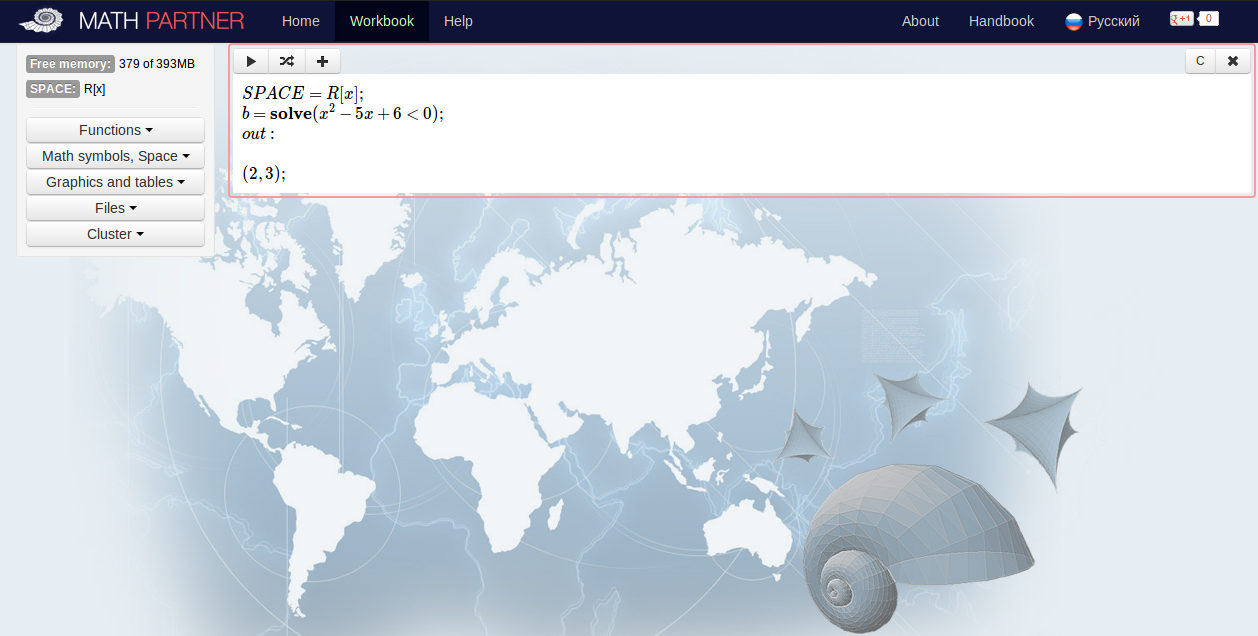
\includegraphics[scale=0.5]{pictures/1_1e}
  \caption{Entering data into a working page}
\end{figure}
%enddelete

On the top of the screen you can see buttons ${\small \fbox {Help}}$ and ${\small \fbox{Handbook}}$. 
This is way to the help files. All the fields of the help pages are active, and you can run the help examples. You can copy text from the samples and transfer them into the field for user input.

When you enter mathematical expressions, they must be separated by a semicolon (;) or text comments, which are enclosed in quotation marks.
 
When you need to have a mathematical expression in the comment as part of the comment, it must be skirted in the dollar signs ($\$$). For example, you can write a comment:

\noindent
$"$ Two different notations $\$ \backslash exp(x)\$$ and $\$\backslash e  \widehat{\ }{} x\$$  are used for the exponential function.$"$

To obtain results it is necessary to use the command \comm{print}{()} and to specify the names of those
 expressions which are required to be printed. 

If the list of statement does not contain a print statement \comm{print}{()} or any other operator (\comm{plot}{()}, \comm{prints}{()}, etc.),  it will be shown the result obtained in the last statement.
  
All commands or operators should begin with the symbol <<back slash>> ($\backslash$).  
 
 
The button $\fbox{+}$ lets us add new entry fields. You can press the combination of
 keys {\it Crtl+Del} to remove this field or you can press the button $\fbox{x}$ at the right side of this field on the screen.
 
The button $\fbox{C}$ is designed to clean the values of all previously typed names. 
It is useful to have such button when the numerical values are entered in some sections, and the calculations are done in other sections. 
Clearing all names allows you to obtain a symbolic expression rather than the number.

On the left of the screen you can see fields with a current environment and a current random access memory. Under the fields differant buttons for enter of functions are placed.


\subsection{Working with files}
Functions for working with files are available at the "Files" collapsible panel from menu at the left.

Here is what you can do with files:

1) Save the result of the last run section as PDF file with "Save PDF" button. You can specify desirable
paper size (dimensions are in centimeters), by default page has size A4 (21x29.7 cm)

2) Upload text files to Mathpar server with "Upload file" button. 
Under the button there is a list of uploaded files. 
Files should contain Mathpar expressions or tables in specific format.

Table contains of header -- it's the first row with arbitrary strings in it -- and
number rows. Columns are separated with tabulation symbol. Functions for working 
with tables are available at the panel "Graphics and tables" (see also 
section 3.1 Plotting functions of help system).

3) Input Mathpar expressions from uploaded files with \comm{fromFile}{()} function.
E.g., to make an expression from file myfile.txt and assign this expression to 
variable $a$ run: a = \comm{fromFile}{('myfile.txt')}.

\section{Mathematical functions}
The following notations for elementary functions and constants are accepted.
\subsection{Constants}  
\hspace*{4mm}  $\backslash$i~--- imaginary unit, 

 $\backslash$e~--- the basis of natural logarithm,  

 $\backslash$pi~--- the ratio of length of a circle to its diameter,    

 $\backslash$infty~--- infinity sign. 


\subsection{Functions of one argument} 

\hspace*{4mm} $\backslash$ln --- natural logarithm, 

 $\backslash$lg --- decimal logarithm, 

 $\backslash$sin --- sine,  

 $\backslash$cos --- cosine,  

 $\backslash$tg --- tangent,  

 $\backslash$ctg --- cotangent, 

 $\backslash$arcsin --- arcsine, 

 $\backslash$arccos --- arccosine,  

 $\backslash$arctg --- arctangent,  

 $\backslash$arcctg --- arccotangent, 

 $\backslash$sh --- sine hyperbolic, 

 $\backslash$ch --- cosine hyperbolic, 

 $\backslash$th --- tangent hyperbolic, 

 $\backslash$cth --- cotangent hyperbolic, 

 $\backslash$arcsh --- arcsine hyperbolic, 

 $\backslash$arcch --- arccosine hyperbolic,  

 $\backslash$arcth --- arctangent hyperbolic, 

 $\backslash$arccth --- arccotangent hyperbolic, 

 $\backslash$exp --- exponent,  

 $\backslash$sqrt --- root square, 

 $\backslash$abs --- absolute value of real numbers (module for complex numbers),

 $\backslash$sign --- number sign (returns $1$, $0$, $-1$ when number sign is $+$, $0$, $-$, correspondingly),
 
 $\backslash$unitStep$(x,a)$ --- is a function which, for $ x> a $ takes the value $ 1 $, and
for $ x <a $ takes the value $ 0 $;

 $\backslash$fact --- factorial.  It is defined for positive integers. It is equivalent to  $n!$.

\subsection{Functions of two arguments} 
\hspace*{4mm}  $\widehat{\ }{}$ --- degree, 

 $\backslash$log --- logarithm of function with given base, 

 $\backslash$rootOf(x, n) --- root of degree n of x, 

 $\backslash$Gamma --- the function Gamma, 

 $\backslash$Gamma2 --- the function Gamma 2,  

 $\backslash$binomial --- binomial coefficient. 


\smallskip

\underline{Example.}

\vspace*{-3mm}
\begin{verbatim}
SPACE = R64[x, y];
f1 = \sin(x);
f2 = \sin(\cos(x + \tg(y)));
f3 = \sin(x^2) + y;
\print(f1, f2, f3);
\end{verbatim}\vspace*{-3mm}
%begindelete

Returns:\\
$SPACE=R64[x,y];$\\
$f1 = sin(x);$\\
$f2 = sin(cos(x+tg(y)));$\\
$f3 = sin(x^{2})+y.$
%enddelete

\section{Actions with functions}

For the above functions and their compositions, you can calculate the value of the function at the point,   substitute the expression into a function instead of arguments, calculate the limit of the function,  calculate derivative, etc. For this purpose, the following commands are defined.



To calculate the value of a function at a point you must run 
\comm{value}{(f, [var1, var2, \ldots, varn])},
where $f$~---function, and 
$var1, var2, \ldots, varn $~--- values 
of the variables of the 
ring.

 For the substitution of expressions to the function you must execute the 
\comm{value}{(f, [func1, func2, \ldots, funcn])}, where $ f $~--- a function
$ func1, func2, \ldots, funcn $~--- expressions that are substituted for the corresponding variables.

 To calculate the limit of a function at a point you must run 
\comm{lim}{(f, var)},
where $ f $~--- this function, and $ var $~--- the point at which you want to find the limit.

 In order to calculate the derivative of 
$f$ in the variable 
$y$ in the ring $\mathbb {Z} [x, \ y, \ z]$
  you must run \comm{D}{(f, y)}. To find a mixed first-order derivative of the function $ f $ there is a command
\comm{D}{(f, [x, y])}, to find the derivative of higher order you must use the command  $\backslash {\mathbf {D}} (f, [x \widehat{\ }{} k, z \widehat{\ }{} m, y \widehat{\ }{} n])$, 
where $ k, m, n $ indicate the order of the derivative of variables.




\smallskip

\underline{Examples. }

\vspace*{-2mm}
\begin{verbatim}
SPACE = R[x, y];
f = \sin(x^2 + \tg(y^3 + x));
g = \value(f, [1, 2]);
\print(g);
\end{verbatim}\vspace*{-2mm}
%begindelete

Returns:\\
in: $SPACE=R[x, y];$\\ 
\hspace*{4mm} $f=sin(x^2+tg(y^3+x)); $\\
\hspace*{4mm} $g=value(f,\ [1,\ 2]); $\\
\hspace*{4mm} $print(g);$\\
out: $g = 0. 52;$\\

%enddelete
\vspace*{-2mm}
\begin{verbatim}
SPACE = Z[x, y];
f = x + y;
g = f^2;
r = \value(f, [x^2, y^2]);
\print(g, f, r);
\end{verbatim}\vspace*{-2mm}
%begindelete

Returns: \\
in: $SPACE=Z[x, y]; $\\
\hspace*{4mm} $f=x+y;$\\ 
\hspace*{4mm} $g=f^2; $\\
\hspace*{4mm} $r=value(f, [x^2, y^2]); $\\
\hspace*{4mm} $print(g, f, r);$\\
out: $g = y^{2}+2yx+x^{2}; $ \\
\hspace*{4mm} $f = y+x;$ \\ 
\hspace*{4mm} $r=x^2+y^2 $

%enddelete
\vspace*{-3mm}
\begin{verbatim}
SPACE = R64[x];
f = \sin(x) / x;
g = \lim(f, 0);
\print(g);
\end{verbatim}\vspace*{-3mm}
%begindelete

Returns: \\
in: $ SPACE=R64[x]; $\\
\hspace*{4mm} $f=sin(x)/x; $\\
\hspace*{4mm} $g=lim(f, 0); $\\
\hspace*{4mm} $print(g);$\\
out: $g = 1. 00;$

%enddelete
\vspace*{-3mm}
\begin{verbatim}
SPACE = Z[x, y];
f = \sin(x^2 + \tg(y^3 + x));
h = \D(f, y);
\print(h);
\end{verbatim}\vspace*{-3mm}
%begindelete

Returns:\\
in: $SPACE=Z[x, y]; $\\
\hspace*{4mm} $f=sin(x^2+ tg(y^3+x)); $\\
\hspace*{4mm} $h= D(f, y);$\\ 
\hspace*{4mm} $print(h);$\\
out: $h = 3y^2 cos(x^2+tg(y^3+x))/(cos(y^3+x))^2;$
%enddelete

\section{Solution of the algebraic equation}  
 
To obtain a solution of the algebraic equation use the command  \comm{solve}{}.

 The command <<FLOATPOS = N>> is used for setting the environment. It sets the number of decimal places after the decimal point $ (N) $, which should appear in the print of the numerical results of approximate calculations. It is not connected with the process of calculation, but only with printing. By default, $ FLOATPOS = 2 $.

\underline{Examples. }

\vspace*{-2mm}
\begin{verbatim}
SPACE = R64[x];
b = \solve(x^2 - 5x + 6 = 0);
\end{verbatim}
%begindelete

\ex{$SPACE=R64[x]; $\\
\hspace*{4mm} $b=solve(x^2-5x+6=0);$ }{$[2. 00, 3. 00];$}

%enddelete
\begin{verbatim}
SPACE = R64[x];
FLOATPOS = 6;
b = \solve(x^4 + 2x + 1 = 0);
\end{verbatim}
%begindelete

\ex{$SPACE=R64[x];$\\ 
\hspace*{4mm} $FLOATPOS=6; $\\
\hspace*{4mm} $b=solve(x^4 +2x +1=0);$}{$[-0.543689,-1.000000];$} 

%enddelete
\begin{verbatim}
SPACE = R64[x];
FLOATPOS = 0;
b = \solve(x^3 + 3x^2 + 3x + 1 = 0);
\end{verbatim}
%begindelete

\ex{$SPACE=R64[x]; $\\
\hspace*{4mm} $FLOATPOS=0;$\\
\hspace*{4mm} $b=solve(x^3+3x^2+3x+1=0);$}{$-1$.}
%enddelete

\section{Solution of the algebraic inequalities}

To obtain a solution of the algebraic inequalities use the command  \comm{solve}{}, which contains the inequalities.
We can solve strict and not strict algebraic inequalities. Open interval is indicated in parentheses ( ), closed interval is indicated inbrackets [ ], set is denoted by braces \{ \}.

\underline{Examples. }

\begin{verbatim}
SPACE = R[x];
b = \solve(x^2-5x+6 < 0);
\end{verbatim}
%begindelete

\ex{$SPACE=R[x]; $\\
\hspace*{4mm} $b=solve(x^2-5x+6 < 0);$}{$(2,3)$.}
%enddelete

\begin{verbatim}
SPACE = R[x];
b = \solve((x+1)^2(x-3)(x+5) \ge 0);
\end{verbatim}
%begindelete

\ex{$SPACE=R[x]; $\\
\hspace*{4mm} $b=solve((x+1)^2(x-3)(x+5) \ge 0);$}{$(-\infty,-5] \cup\{-1\}\cup[3,\infty)$.}
%enddelete

\begin{verbatim}
SPACE = R[x];
b = \solve((x^2+11x+28)/(x+5) \le 0);
\end{verbatim}
%begindelete

\ex{$SPACE=R[x]; $\\
\hspace*{4mm} $b=solve((x^2+11x+28)/(x+5) \le 0);$}{$(-\infty,-7]\cup(-5,-4]$.}
%enddelete

\begin{verbatim}
SPACE = Q[x];
b = \solve(x^2 + 4x - 7 = 0);
\end{verbatim}
%begindelete

\ex{$SPACE=Q[x]; $\\
\hspace*{4mm} $b=solve((x^2 + 4x - 7 = 0);$}{$[(\sqrt{11}+(2)),(2-\sqrt{11})];$.}
%enddelete
\section{Solution of the algebraic inequalities systems}

To obtain a solution of the algebraic inequalities systems use the command \comm{solve}{[In1, In2, ..., Ink]}, where $[In1, In2, ..., Ink]$~--- vector, where contain inequalities.
System contain strict and not strict algebraic inequalities. Open interval is indicated in parentheses (), closed interval is indicated inbrackets, set is denoted by braces \{ \}.

\underline{Examples. }

\vspace*{-2mm}
\begin{verbatim}
SPACE = R[x];
b = \solve([x^2+4x-5 > 0, x^2-2x-8 < 0]);
\end{verbatim}
%begindelete

\ex{$SPACE=R[x]; $\\
\hspace*{4mm} $b=solve([x^2+4x-5 > 0, x^2-2x-8 < 0]);$}{$(1,4)$.}
%enddelete

\begin{verbatim}
SPACE = R[x];
b = \solve([x^2-x-6 \ge 0, x^2-4x-12 < 0]);
\end{verbatim}
%begindelete

\ex{$SPACE=R[x]; $\\
\hspace*{4mm} $b=solve([x^2-x-6 \ge 0, x^2-4x-12 < 0]);$}{$(-4,-2]\cup[3,4)$.}
%enddelete

\begin{verbatim}
SPACE = R[x];
b = \solve([x^2-4 < 0, x+1 > 0, 0.5-x > 0]);
\end{verbatim}
%begindelete

\ex{$SPACE=R[x]; $\\
\hspace*{4mm} $b=solve([x^2-4 < 0, x+1 > 0, 0.5-x > 0]);$}{$(-1,0.5)$.}
%enddelete

\section{Operations on subsets of the real numbers}

To specify a subset use the command \comm{set}{((a,b),(c,d])}, where $a,b,c,d$ are numbers.
Subset may consist of open intervals indicated by parentheses ( ), half-open intervals indicated by [ ) or ( ],
segments indicated by brackets [ ] and points indicated by braces { }, or like segments.

Simple subset is denoted by the same brackets, but you need to add a backslash ($ \backslash $) in front of each bracket. 
For example $ \backslash (3,4.5) \backslash] $, $ \backslash[7, 7 \backslash]$ or $\backslash{8 \backslash}$.
The operator $ \backslash {\mathbf {set}} $ is not required.

\begin{verbatim}
SPACE = R64[x];
a = \set((-2,1),[2,5),(5.75,6],[8,8]);
\end{verbatim}
%begindelete

\ex{$SPACE=R[x]; $\\
\hspace*{4mm} $a = set((-2,1),[2,5),(5.75,6],{8});$}{$((-2.00),1.00)\cup[2.00,5.00)\cup(5.75,6.00]\cup\{8.00\}$.}
%enddelete
 

With subsets we can make the following operations: union, intersection, subtraction, calculation of 
the symmetric difference and complement set, using the commands $\backslash cup$, 
$\backslash cap$, $\backslash setminus$, $\backslash triangle$ and symbol  (') apostrophe.

 
 
\begin{verbatim}
SPACE = R64[x];
A=\(1,3\)\cup\[5,16\);
B=\(2,4\)\cup\[10,20\);
C=A\cup B;
D=A\cap B;
E=A\triangle B;
F=A \setminus B;
G=A';
\print(C,D,E,F,G);
\end{verbatim}
%begindelete

\ex{ $SPACE=R64[x]; $\\
$ A=(1,3)\cup[5,16);$\\
$B=(2,4)\cup[10,20);$\\
$C=A\cup B;$\\
$D=A\cap B;$\\
$E=A\triangle B;$\\
$F=A \setminus B;$\\
$G=A';$\\
$print(C,D,E,F,G);$}
{$C = (1,4)\cup[5,20)$\\
 $D = (2,3)\cup[10,16)$\\
 $E = (1,2]\cup[3,4)\cup[5,10)\cup[16,20)$\\
 $F = (1,2]\cup[5,10)$\\
 $G = (-\infty,1]\cup[3,5)\cup[16,\infty)$}
%enddelete


\newpage
\section{Vectors and matrices}
To define the row-vector you have to list its elements in square brackets. 

To define the matrix you must take in square brackets a list of row vectors, for example, $ A = [[1, 2], [3, 4]] $.

Element of the matrix may be obtained by specifying the row and column number in the two lower indexes of the matrix,
and an element of the vector may be obtained by specifying its number in the lower index of the vector.
The is an example for obtaining elements. You have to set $a=\backslash elementOf(A)$, and then obtain $a$\_\{$i, j$\}.  If $B$ is a vector, then you have to set $b=\backslash elementOf(B)$, and then obtain element $b$\_\{$i$\}.  
 
You can get a row of the matrix as a vector-row and column of the matrix as a column vector. The row vector obtained by specifying the number of row in the first index and a  sign of question <<?>> in the second index, for example, $a$\_\{$i, ?$\}. Column vector obtained by specifying the number of column in the second index and the  sign of question <<?>> in the first index, for example, $a$\_\{$?, j$\}.
 
The names of non-commutative objects, such as matrices and vectors, must be written with the symbol <<back slash>> ($\backslash$) and a capital letter.


To denote zero and identity matrix you can 
use the caps $\backslash O$ and $\backslash I$, with two indexes, 
indicating the number of 
rows and columns. With the help of the symbol $\backslash I $, you can create any size square matrix whose elements on the 
main diagonal are equal to $ 1 $, and the remaining elements are zero. For example, $\backslash I$\_\{$2, 3$\} and $\backslash O$\_\{$2, 2$\} denote the matrix 
$ \left(\begin {array} {ccc}
1 & 0 & 0 \\ 0 & 1 & 0 \\ 
\end {array} \right) $ 
and $ \left(\begin {array} {cc}
0 & 0 \\ 0 & 0 \\ \end {array} \right) $. You can specify zero vectors, indicating the index number of elements: $\backslash O$\_\{$3$\} denote the vector $ [0, \ 0, \ 0] $ and $I$\_\{$3$\}   denotes the vector $ [ 1, \ 0, \ 0] $.

Column vector can be formed by transposing the row vector, for example, $ D = [7, \ 2, \ 3] ^ T $~--- it is a column vector with three elements.
 
Arithmetic operations are indicated by standard signs ``~+~'',~``~-~'', ``~*~''.

\smallskip

%begindelete
\underline{Example 1. }
%enddelete 
\begin{verbatim}
SPACE = Z[x];
A = [[x, 4], [y, 5]];
V = [x, y, 1, 2, x^6];
\print(A, V);
\end{verbatim}
%begindelete

\ex{$SPACE=Z[x];$ \\
\hspace*{4mm} $A =\left(\begin{array}{cc}x &4 \\ y &5 \end{array}\right) ; $\\
\hspace*{4mm} $V = [x, y, 1, 2, x^6];$ \\
\hspace*{4mm} $print(A, V);$}{$A =\left(\begin{array}{cc}x &4 \\ y &5 \end{array}\right) ; $\\
\hspace*{4mm} $V = [x, y, 1, 2, x^{6}];$}

\underline{Example 2. }
%enddelete
\begin{verbatim}
SPACE = Z[x, y];
A = [[3, 4], [3, 1]];
B = [[2, 5], [4, 7]];
C = A + B;
G = A - B;
T = A * B;
\print(C, G, T);
\end{verbatim}
%begindelete

\ex{$SPACE=Z[x];$ \\
\hspace*{4mm} $A=\left(\begin{array}{cc}3& 4\\ 3& 1\\ \end{array}\right) ; $\\
\hspace*{4mm} $B=\left(\begin{array}{cc}2& 5\\ 4& 7\\ \end{array}\right);  $\\
\hspace*{4mm} $C=A+B; $\\
\hspace*{4mm} $G=A-B; $\\
\hspace*{4mm} $T=A*B; $\\
\hspace*{4mm} $print(C, G, T);$}{$C =\left(\begin{array}{cc}5 &9 \\ 7 &8 \end{array}\right) ; $\\
\hspace*{4mm} $G =\left(\begin{array}{cc}1 & -1 \\ -1 &-6 \end{array}\right) ; $\\
\hspace*{4mm} $T =\left(\begin{array}{cc}22 &43 \\ 10 &22 \end{array}\right) ;$}

\underline{Example 3. }
%enddelete
\begin{verbatim}
SPACE = Z[x];
A = [[1, 4], [-4, 5]];
a = \elementOf(A);
det = a_{1, 1} * a_{2, 2} - a_{1, 2} * a_{2, 1};
\print(det);
\end{verbatim}
%begindelete

\ex{$SPACE=Z[x];$ \\
\hspace*{4mm} $A=\left(\begin{array}{cc}1& 4\\ -4& 5\\ \end{array}\right); $\\
\hspace*{4mm} $det=a_{1, 1}*a_{2, 2}-a_{1, 2}*a_{2, 1}; $ \\
\hspace*{4mm} $print(det);$}
{$det = 21;$}

\underline{Example 4. }
%enddelete
\begin{verbatim}
SPACE = Z[x, y];
A = [[x^2, y], [4, x+y]];
a = \elementOf(A);
B = a_{1, ?};
C = a_{?, 2};
b = \elementOf(B);
c = \elementOf(C);
h = b_{2} * c_{1, 1};
\print(B, C, h);
\end{verbatim}
%begindelete

\ex{$SPACE=Z[x, y];$ \\ 
\hspace*{4mm} $A=\left(\begin{array}{cc}x^2& y\\ 4& x+y\\ \end{array}\right); $ \\
\hspace*{4mm} $a=\backslash elementOf(A);$ \\
\hspace*{4mm} $B=a_{1, ?}; $ \\
\hspace*{4mm} $C=a_{?, 2};  $ \\
\hspace*{4mm} $b=\backslash elementOf(B); c=\backslash elementOf(C); $ \\
\hspace*{4mm} $h=b_{2} \cdot c_{1}; $ \\
\hspace*{4mm} $print(B, C, h);$ } {$B =\left(\begin{array}{cc}x^{2}   \\ 4   \end{array}\right) ; $ \\ 
\hspace*{4mm} $C =\left(\begin{array}{cc}4 & y+x \end{array}\right) ; $ \\
\hspace*{4mm} $ h = (y^2); $}

\underline{Example 5. }
%enddelete
\begin{verbatim}
SPACE = Z[x, y];
A = 3x * \I_{2, 2};
B = \O_{3, 3};
\print(A, B);
\end{verbatim}
%begindelete

\ex{$ SPACE=Z[x, y]; $ \\
\hspace*{4mm} $A=3x* {\mathbf I}_{2, 2}; $ \\
\hspace*{4mm} $B={\mathbf O}_{3, 3}; $ \\
\hspace*{4mm} $print(A, B);$ }{$A =\left(\begin{array}{cc}3x &0\\ 0 & 3x \end{array}\right) ; $\\
\hspace*{4mm} $B =\left(\begin{array}{ccc}0 &0 &0 \\ 0 &0 &0 \\ 0 &0 &0 \end{array}\right). $} 
%enddelete

%begindelete
\underline{Example 6. }
%enddelete
\begin{verbatim}
SPACE = R64[x];
A = [\pi / 2, \pi];
B = \sin(A);
C = \value(B);
\print(A, B, C);
\end{verbatim}
%begindelete

\ex{$SPACE = R64[x];$\\
\hspace*{4mm} 
$A = [\pi / 2, \pi];$\\
\hspace*{4mm} 
$B = \sin(A);$\\
\hspace*{4mm} 
$C = value(B);$\\
\hspace*{4mm} 
$print(A, B, C);$}{$A=[\pi/2,\pi]; $ \\
\hspace*{4mm} $B={\mathbf sin} ([\pi/2,\pi]); $ \\
\hspace*{4mm} $C= [1 , 0]; $}
%enddelete

\section{Generation of random elements} 
Mathpar can generate of random elements such as numbers, polynomials and matrices.
\subsection{Generation of numbers} 
To create a random number you have to execute the command 
\comm{randomNumber}{(k)}, where $k$ is the number of bits.

\smallskip

%begindelete

\underline{Example. }

\vspace*{-3mm}
%enddelete

\begin{verbatim}
SPACE = Z[x, y, z];
a = \randomNumber(10);
b = \randomNumber(100);
\print(a, b);
\end{verbatim}
%begindelete

Returns:\\ 
$SPACE=Z[x,y,z]; $\\
$a = 944; $ \\
$b = 850800798881527094755736477974. $
%enddelete

\subsection{Generation of random polynomial} 
To create a random polynomial with three variables you have to execute the command 
\comm{randomPolynom}{(d1, d2,\ldots, ds, dens, bits)}, 
where $dens$ is a polynomial density, $bits$ is a number of bits in numerical coefficients, and $d1, d2, \ldots, ds$ denote the highest degrees of variable.
If $dens=100$, you get a polynomial that has all coefficients
non-zero, all $(d1 +1) (d2 +1) \cdot (ds +1)$ non-zero terms. 
When $ dens < 100$, only $ dens \% $ coefficients are nonzero, 
and the remaining $ (100-dens) \% $ will be zero.

\smallskip

%begindelete
\underline{Example. }

\vspace*{-3mm}
%enddelete

\begin{verbatim}
SPACE=Z[x,y,z];
f = \randomPolynom(4, 4, 10, 5);
g = \randomPolynom(4, 4, 10, 5);
h = f + g;
\print(f, g, h);
\end{verbatim}
%begindelete

Returns: \\ 
$SPACE=Z[x,y,z]; $\\
$f = y^{3}x^{3}; $\\
$g = 10yx^{3}+2y; $\\
$h = y^{3}x^{3}+10yx^{3}+2y; $
%enddelete

\subsection{Generation of random matrix}
To create arandom numerical matrix you have to execute the command 
\comm{randomMatrix}{(m, n, dens, bits)},  
where last two arguments are the density of matrix and the number of bits in numerical elements of matrix, and first two arguments denote the sizes of a matrix. 

To create a polynomial matrix you have to execute the command 
\comm{randomMatrix}{(m, n, dens, d1, d2, \ldots, ds, pol\_dens, pol\_bits))}, 
 where first three arguments denote the size of a matrix and its density, last two arguments are the density of polynomials and the number of bits in numerical coefficients, the numbers $d1, d2,\ldots, ds$ set the highest degrees of polynomial variables.

\smallskip

%begindelete
\underline{Example. }

\vspace*{-3mm}
%enddelete

\begin{verbatim}
SPACE = Z[x, y, z];
matr_n = \randomMatrix(4, 4, 100, 5);
matr_p = \randomMatrix(2, 2, 100, 1, 1, 4, 25, 3);
\print(matr_n, matr_p);
\end{verbatim}
%begindelete

Returns:\\
$SPACE=Z[x,y,z]; $\\
$matr_n =\left(\begin{array}{cccc}22 &2 & 10 &28 \\ 23 &28 &1 & 19 \\ 30 &24 &19 &12 \\ 27 &22 &22 &17 \end{array}\right) ; $ \\
$matr_p =\left(\begin{array}{cc}
6z^3x+7z^3+5z^2+3y & 7z^4x+2z^4+7zyx+5x\\
 z^4yx+2zy+7y+7x+4&  7z^2x+7zx+z+6x \\
 \end{array}\right). $
%enddelete
 

\chapter{Построение 2D и 3D графиков}

\section{Построение графиков функций}
Mathpar позволяет строить табличные графики ($tablePlot$), графики функций, которые заданы явно ($plot$) или параметрически ($paramPlot$). 
Можно строить несколько разных графиков в одной системе координат($showPlots$).
  
Окружение для построения графиков задается командой \comm{set2D}{()}.
Если у команды \comm{set2D}{()} нет параметров, то границы для графиков расчитываются автоматически, а для явных функций выбирается интервал 
$[0,1]$ по оси абсцисс. Наименования осей координат будет $X$ и $Y$, соответственно. Заголовок у графика будет отсутствовать.
   
Если команда \comm{set2D}{()} пользователем не задавалась, то автоматически устанавливается \comm{set2D}{()} без параметров в начале сеанса
данного пользователя.

Cуществует 2 формата -- полный и сокращенный.

 Полный  формат  предполагает 3 группы параметров, каждая из которых 
пишется в квадратных скобках:\\
\comm{set2D}{([x0,x1, y0, y1],['xTitle','yTitle','title'] ,[0,1,12,3,5])}.

Первая кваадратная скобка определяет границы графика. 
Эта скобка должна обязательно присутствовать. 
В первой скобке можно указывать только 2 числа - границы по оси абсцисс, при этом
границы по вертикальной оси расчитываются автоматически.

Вторая  кваадратная скобка это надписи к осям координат и подпись ко всему рисунку.
Если в этой скобке 2 аргумента -- то это первые два -- подписи к осям,
а если только один аргумент -- то это название к рисунку.

Третья  кваадратная скобка содержит 5 чисел: \\
1) 1 -- означает: установить режим черно-белый (0 - цветной)\\
2) 1 -- означает: установить равный масштаб по обеим осям (0- золотое сечение)\\
3)  это размер шрифта для подписей\\
4)  это толщина линий графиков\\
5)  это толщина координатных осей\\

Есть для этой скобки и 3 сокращенных варианта:['ES'],['BW'],['ESBW'].
Они, соответственно, устанавливают в значение 1 или первый параметр, или второй параметр, или оба.

Любая из 2х последних скобок может отсутствовать, могут отсутствовать и обе.

Существует 7  сокращеных вариантов для этой команды: \\
1) \comm{set2D}{()};\\
2) \comm{set2D}{(x0,x1)}; \\
3) \comm{set2D}{(x0,x1,'title')};\\ 
4) \comm{set2D}{(x0,x1,y0,y1)};\\
5) \comm{set2D}{(x0,x1,y0,y1,'title')};\\
6) \comm{set2D}{(x0,x1,'title','nameOX','nameOY')};\\ 
7) \comm{set2D}{(x0,x1,y0,y1,'title','nameOX','nameOY')}.\\ 

Числа $x0$ и $x1$ $(x0<x1)$ задают интервал по оси $OX$. Числа $y0$ и $y1$ $(x0<x1)$ задают интервал по оси $OY$. 
Если эти параметры не заданы, то расчитываются автоматически. $nameOX$~--- подпись на оси $OX$, $nameOY$~--- подпись на оси $OY$, $title$~--- заголовок графика.

Кроме этого, разрешается задать еще один или два ключа, которые должны стоять последними в списке параметров:  $BW$ и $ES$. 
$BW$ указывает на построение черо-белого графика. $ES$ указывает на равенство масштаба шкалы $x$ масштабу шкалы $у$. 
Всего имеется $7*4=28$ разных способов задания параметров окружения.

Характер линии, которая изображается на графике каждой из функций
$(plot, tablePlot, paramPlot)$ может быть разный: сплошная линия, пунктирная линия и линия, которая оканчивается стрелкой. 
Для этого предназначены параметы: '$dash$' (пунктир), '$arrow$' (стрелки) и их сочетание '$dashAndArrow$', которые должны стоять  в конце списка параметров этих функций. 

Например, \comm{plot}{( x^2+1 , 'dash')}.

Если нескольким отдельным графикам присвоены имена, например, 
P=\comm{plot}{(x^2)}; Q=\comm{tablePlot}{([[1,2],[3,4]])}; 
в этом случае их можно изобразить вместе с помощью команды \comm{showPlots}{([P,Q])}.

У этой команды есть дополнительные опции 'noAxes'~--- не изображать оси координат и 'lattice'~--- изображать сетку.
Например, \comm{showPlots}{([P,Q], 'lattice')}. 


Полученный график можно загрузить с сайта.
Для этого под полем ввода нужно кликнуть на кнопку 
$\fbox{%begindelete
\mbox{%enddelete
Загрузить%begindelete
}%enddelete
}$, и файл с графиком будет загружен на компьютер
пользователя.


\subsection{Явное задание функции}
 Для построения графика функции $f=f(x)$ используется команда \comm{plot}{(f)}. 
Другие варианты команд: \\
1) \comm{plot}{(f, [x0, x1])}, где $[x0, x1]$~--- интервал по оси $OX$;\\
2) \comm{plot}{(f, [x0, x1], 'options')}, где $[x0, x1]$~--- интервал по оси $OX$, 'options'~--- принимает следующие значения:\\
1)'dash'~--- график будет изображен пунктиром;\\ 
2)'arrow'~---  последняя точка графика будет нарисована со стрелкой;\\
3)'dashAndArrow'~--- график будет изображен пунктиром и последняя точка графика будет нарисована со стрелкой.\\
3) \comm{plot}{(f, 'options')}.

Можно строить графики функций, содержащих параметры. Эти параметры необходимо определить как переменные в задании окружения (см. пример 3). Параметры могут принимать значения из отрезка $[0;1]$.  Сначала график строится для значений параметров, равных единице. Эти значения можно менять. Для этого надо выбрать имя параметра и передвинуть бегунок до нужного значения, затем нажать на кнопку 
$\fbox{%begindelete
\mbox{%enddelete
Построить%begindelete
}%enddelete
}$. 

%begindelete
\underline{Пример 1. }
%enddelete
\vspace*{-2mm}
\begin{verbatim}
SPACE = R64[x, y, z];
\set2D(-10, 10, -10, 10);
f = x^2 + \tg(x^2 - 1); 
p = \plot(f);
\end{verbatim}
\vspace*{-2mm}
%begindelete 
  
\ex{$f=x^2+\tg(x^2-1);$}
{рис. \ref{3_1}.}

\begin{figure}[h!]
  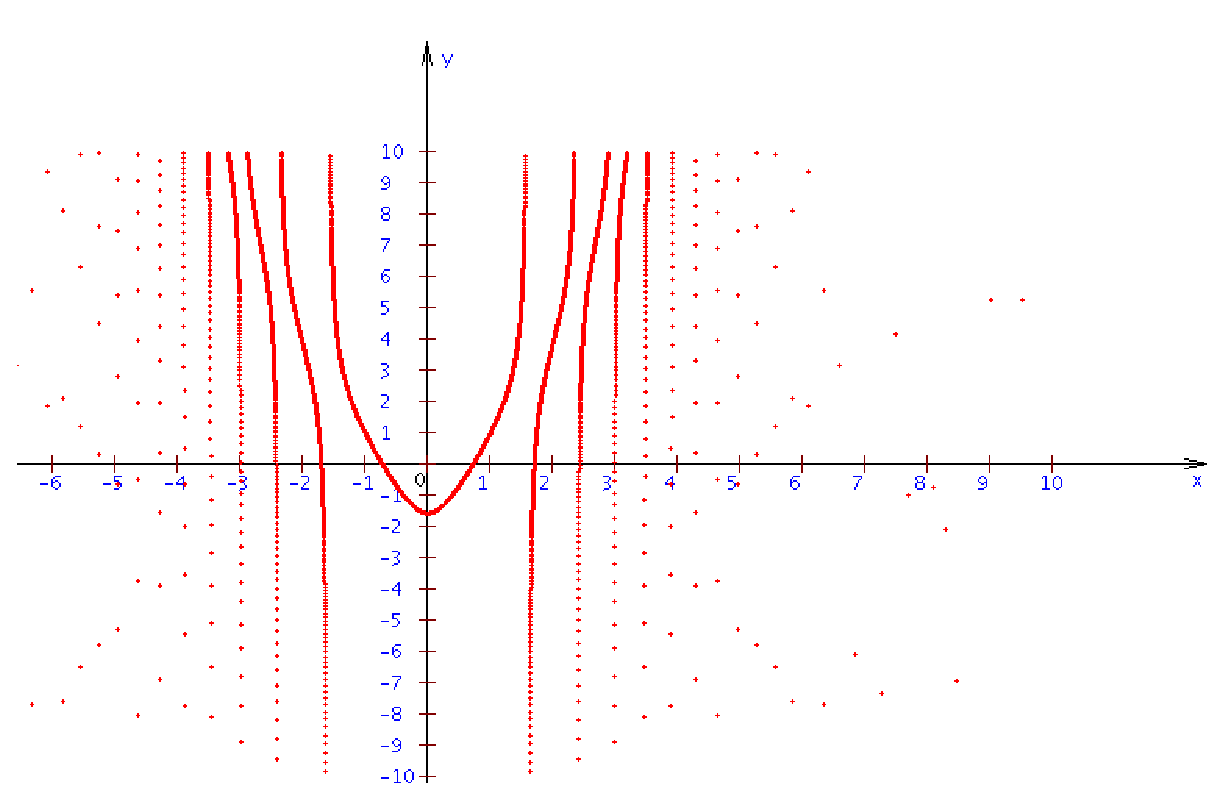
\includegraphics[scale=0.45]{pictures/3_1}
  \caption{График функции $f=x^2+\tg(x^2-1)$}
  \label{3_1}
\end{figure}

\eject

Чтобы получить графики нескольких функций на одном рисунке нужно список
этих функций заключить в квадратные скобки, как в следующем примере.

\underline{Пример 2. }

%enddelete

\begin{verbatim}
SPACE = R64[x, y, z];
\set2D(-10, 10, -10, 10);
f = \sin(x); 
p = \plot([f, \tg(x)]);
\end{verbatim}
%begindelete

\ex{$f=sin(x);$}{рис. \ref{3_3}.}

\begin{figure}[!h]
  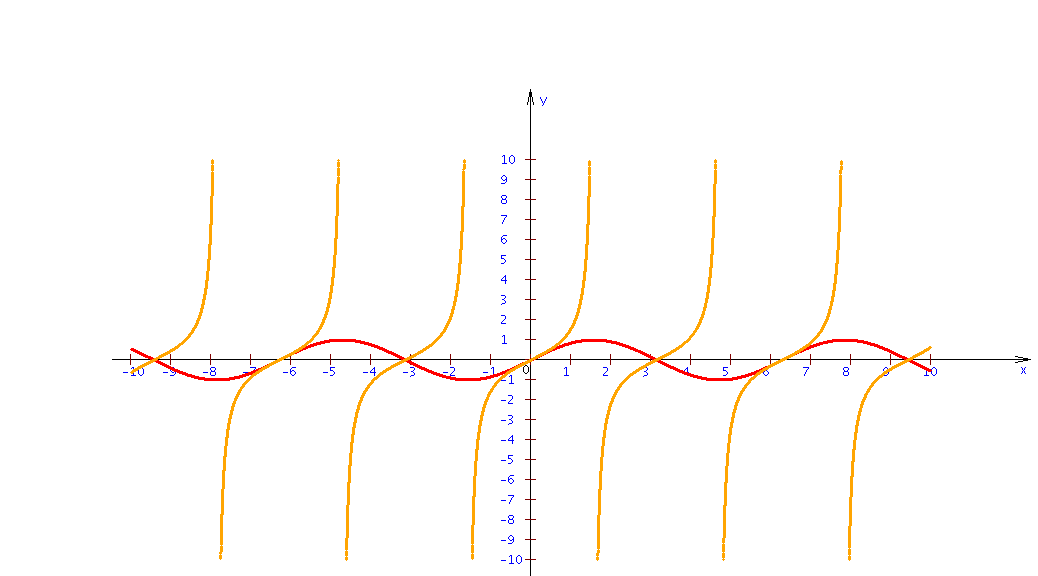
\includegraphics[width=274.6pt,height=152.38pt]{pictures/3_3}
  \caption{Графики функций $f = \sin(x)$ и $g = \tg(x)$}
  \label{3_3}
\end{figure}

\underline{Пример 3. }

%enddelete

\begin{verbatim}
SPACE = R64[x, y, z];
\set2D(-10, 10, 0, 2);
f = \unitBox(x,3); 
p = \plot(f);
\end{verbatim}
%begindelete

%\ex{$f=sin(x);$}{рис. \ref{3_3}.}

%\begin{figure}[!h]
%  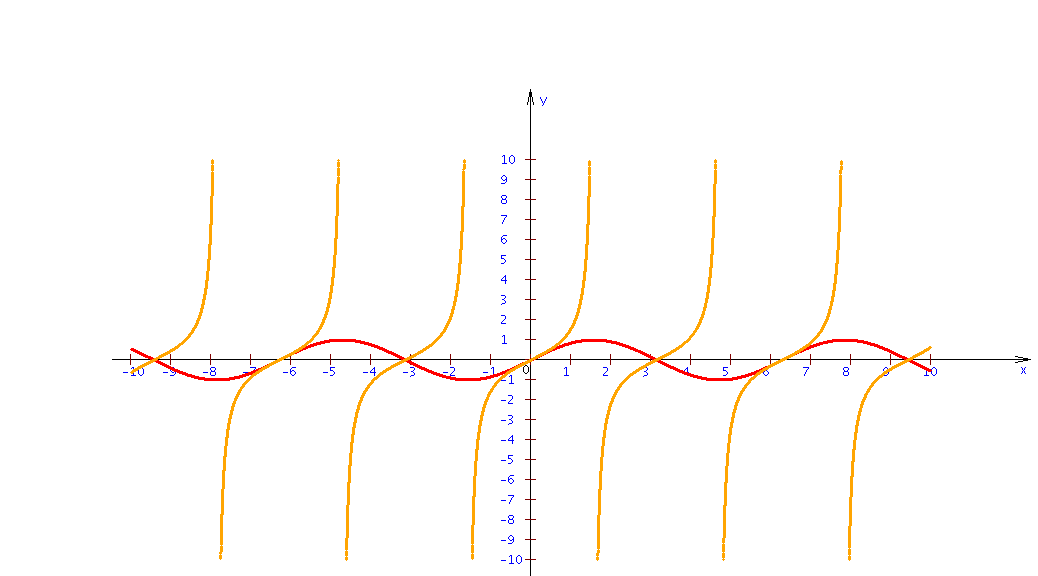
\includegraphics[width=274.6pt,height=152.38pt]{pictures/3_3}
%  \caption{Графики функций $f = \sin(x)$ и $g = \tg(x)$}
%  \label{3_3}
%\end{figure}

\underline{Пример 4. }

%enddelete

\begin{verbatim}
SPACE = R64[x, a, b, c];
\set2D(0, 2\pi, 0, 2);
\plot(a\sin(bx) + c);
\end{verbatim}

%begindelete

%  \ex{$f=sin(x);$}{pict. \ref{3_3}. }
% 
% \begin{figure}[!h]
%   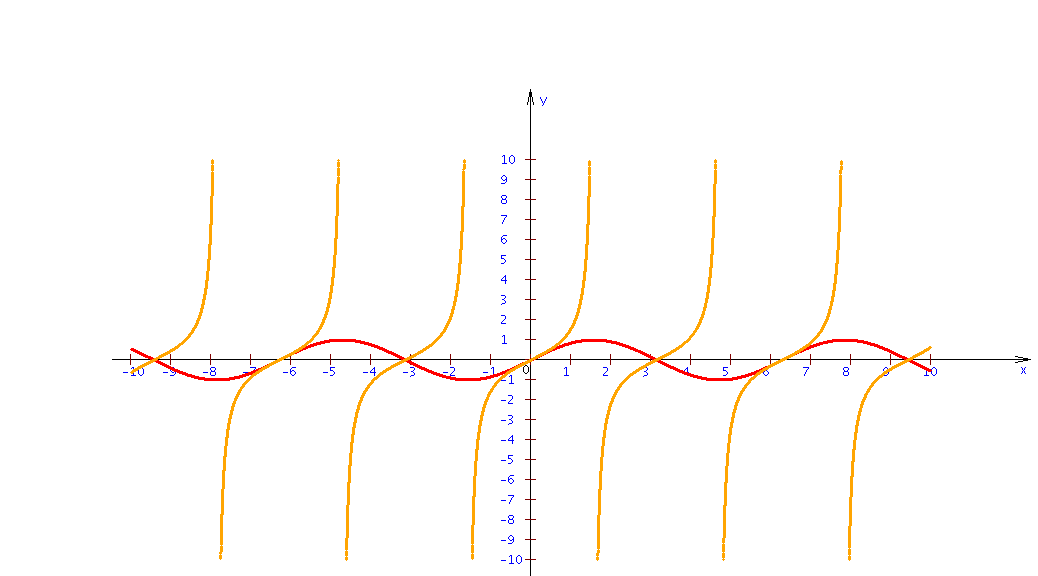
\includegraphics[width=274.6pt,height=152.38pt]{pictures/3_3}
%   \caption{Графики функций $f = \sin(x)$ и $g = \tg(x)$}
%   \label{3_3}
% \end{figure}
%enddelete

%begindelete
\underline{Пример 5. }
%enddelete
\vspace*{-2mm}
\begin{verbatim}
SPACE = R64[x, y, z];
\set2D(-10, 10, -10, 10,'a','b','title');
f = x^2; 
p = \plot(f);
\end{verbatim}
\vspace*{-2mm}

%begindelete
\underline{Пример 6. }
%enddelete
\vspace*{-2mm}
\begin{verbatim}
SPACE = R64[x, y, z];
\set2D(-10, 10, -10, 10);
f = x; 
p = \plot(f,'dash');
\end{verbatim}
\vspace*{-2mm}

%begindelete
\underline{Пример 7. }
%enddelete
\vspace*{-2mm}
\begin{verbatim}
SPACE = R64[x, y, z]; 
f = x; 
p = \plot(f,[-5,5],'arrow');
\end{verbatim}
\vspace*{-2mm}

%begindelete
\underline{Пример 8. }
%enddelete
\vspace*{-2mm}
\begin{verbatim}
SPACE = R64[x, y, z]; 
\set2D(-10, 10, -10, 10);
\plot([x,-x],'arrow');
\end{verbatim}
\vspace*{-2mm}

%begindelete
Для построения графика функции во времени с изменением параметров необходимо указать количество кадров - (например установим: frames = 5) (см. Рис.1.)

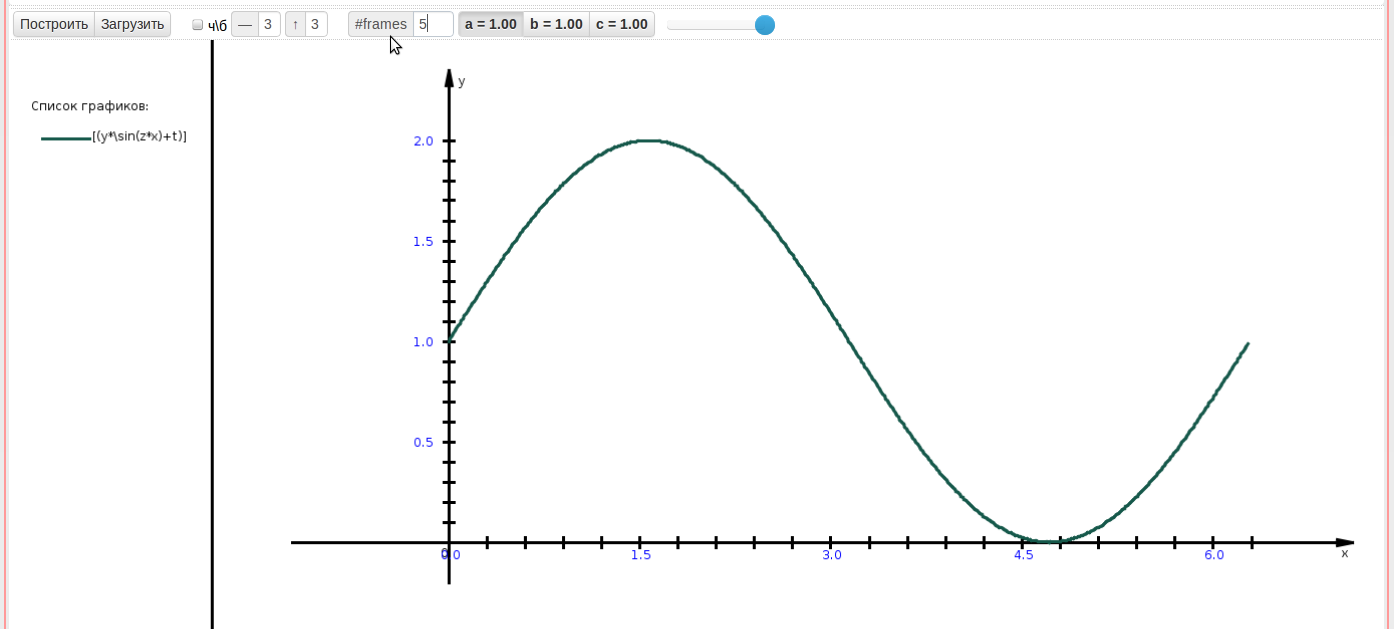
\includegraphics[scale=0.35]{pictures/2_9}

Для изменения параметров используйте ползунок - (например установим: a = 0.2, b = 0.4, c = 0.6) (см. Рис.2.)

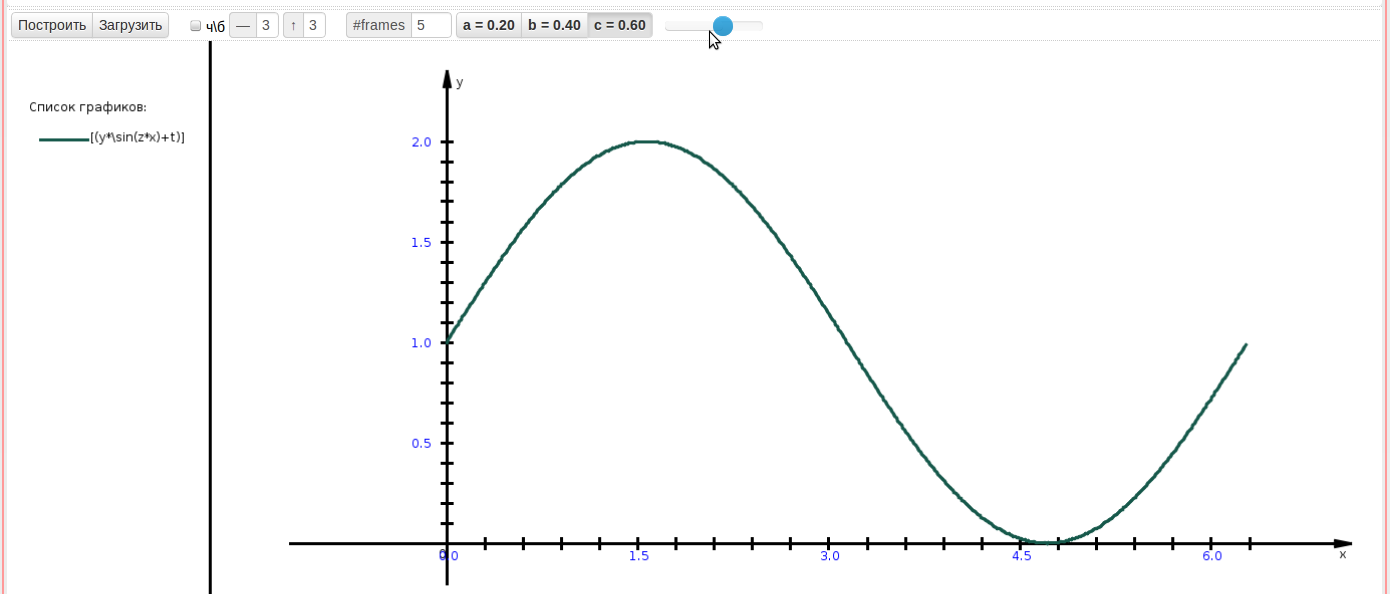
\includegraphics[scale=0.35]{pictures/2_10}

Для построения графика нажимаем кнопку - 'Построить' (см. Рис.3.)

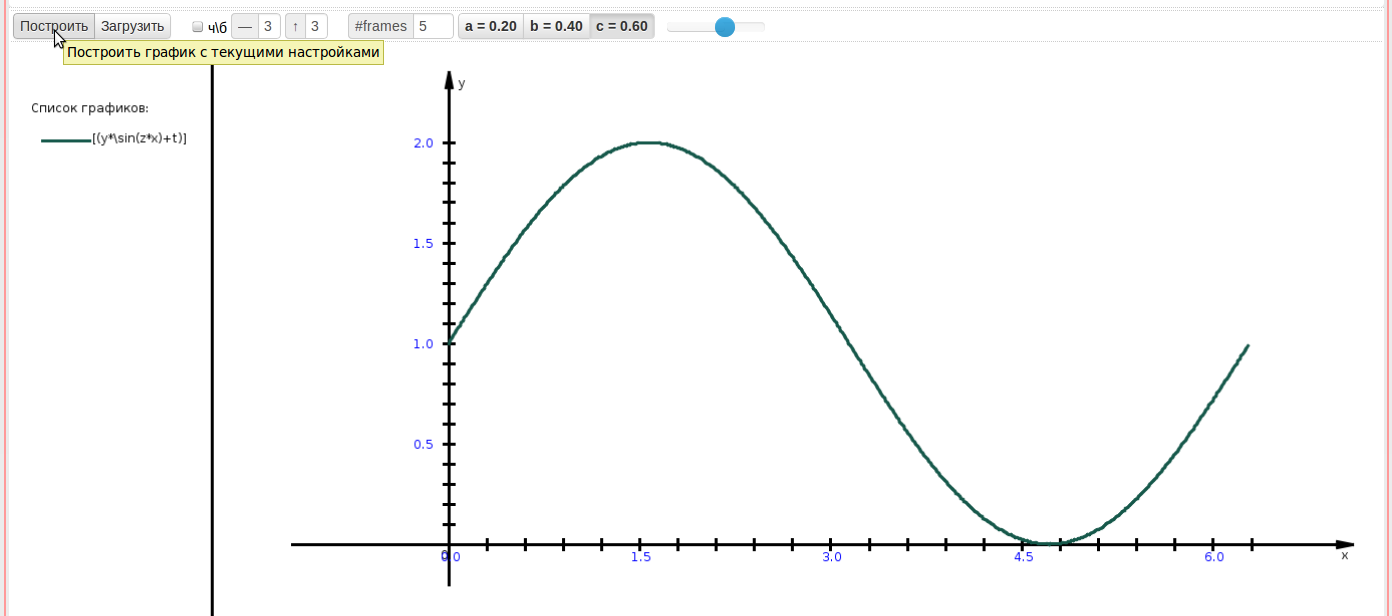
\includegraphics[scale=0.35]{pictures/2_11}

В результате получаем график.(см. Рис.4.)

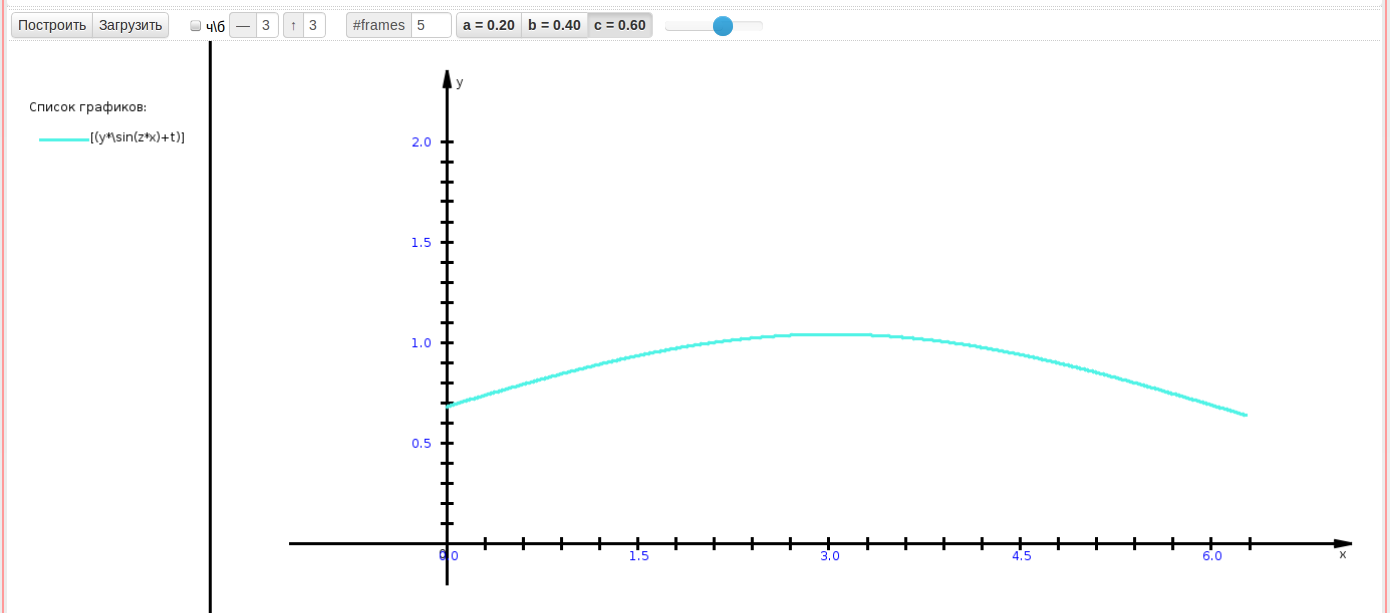
\includegraphics[scale=0.35]{pictures/2_12}

%enddelete

\subsection{Функции, заданные параметрически}
Для построения графиков функций, которые заданы параметрически,  необходимо выполнить команду 
\comm{paramPlot}{([f, g], [t0, t1])}, 
где $f = x(t)$, $g = y(t)$~--- функции,  заданная параметрически, 
$[t0, t1]$~--- интервал значений для изменения параметра. 
Другой вариант команды: \comm{paramPlot}{([f, g], [t0, t1], 'options')}, где $[t0, t1]$~--- интервал значений для изменения параметра, 
$'options'$~--- принимает следующие значения:\\
1)$'dash'$~--- график будет изображен пунктиром;\\ 
2)$'arrow'$~---  последняя точка графика будет нарисована со стрелкой;\\
3)$'dashAndArrow'$~--- график будет изображен пунктиром и последняя точка графика будет нарисована со стрелкой.\\


%begindelete
\underline{Пример 1. }


\nopagebreak
%enddelete
\vspace*{-2mm}
\begin{verbatim}
SPACE = R64[x, y, z];
g = \sin(x); 
k = \cos(x); 
f = \paramPlot([g, k], [0, 2\pi]);
\end{verbatim}
\vspace*{-2mm}

%begindelete
\ex{$g=sin(x); k=cos(x);$}{рис. \ref{3_4}.}
\begin{figure}[h!]
 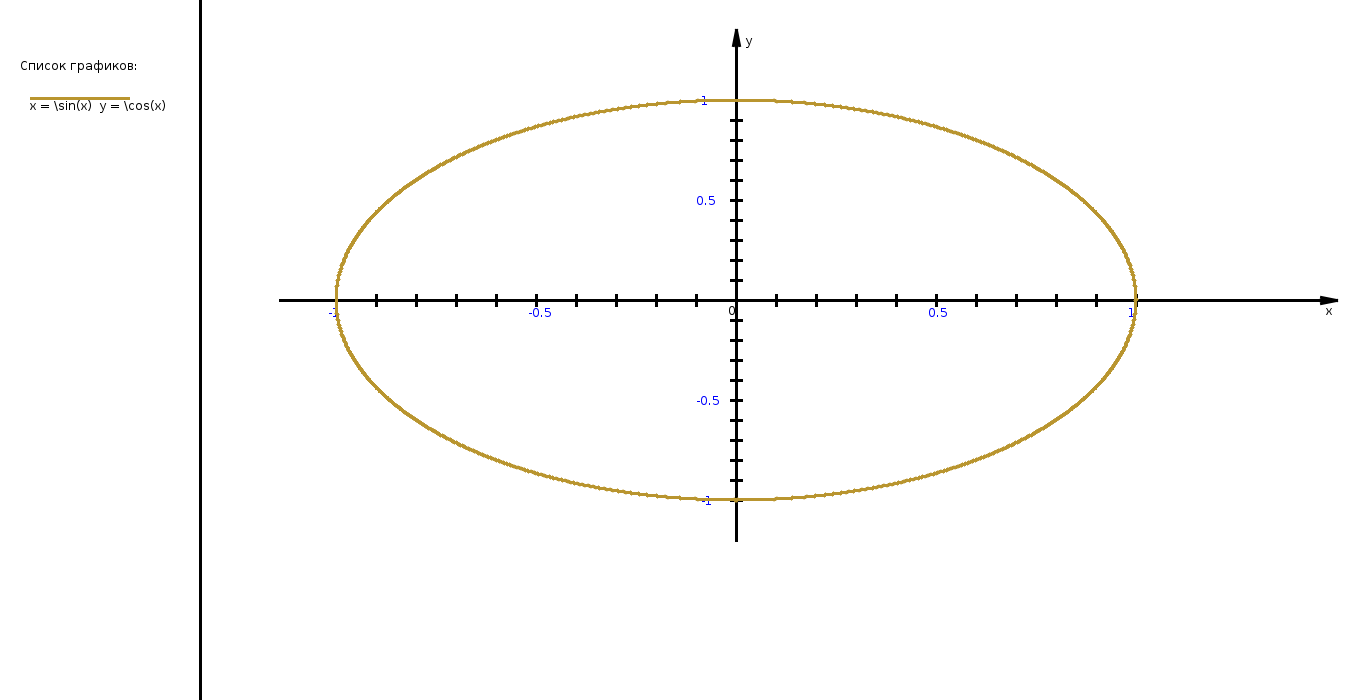
\includegraphics[scale=0.26]{pictures/2_1}
\vspace*{-10mm}
\caption{График функции, заданной параметрически}
\label{3_4}
\end{figure}
%enddelete


%begindelete
\eject
\underline{Пример 2. }


%enddelete
\vspace*{-2mm}
\begin{verbatim}
SPACE = R64[x, y, z];
g = x\sin(x);
k = x\cos(x);
f = \paramPlot([g, k], [0, 5\pi]);
\end{verbatim}
\vspace*{-2mm}

%begindelete
\ex{$g=x\sin(x); k=x\cos(x);$}{рис. \ref{2_2}.}
\begin{figure}[h!]
 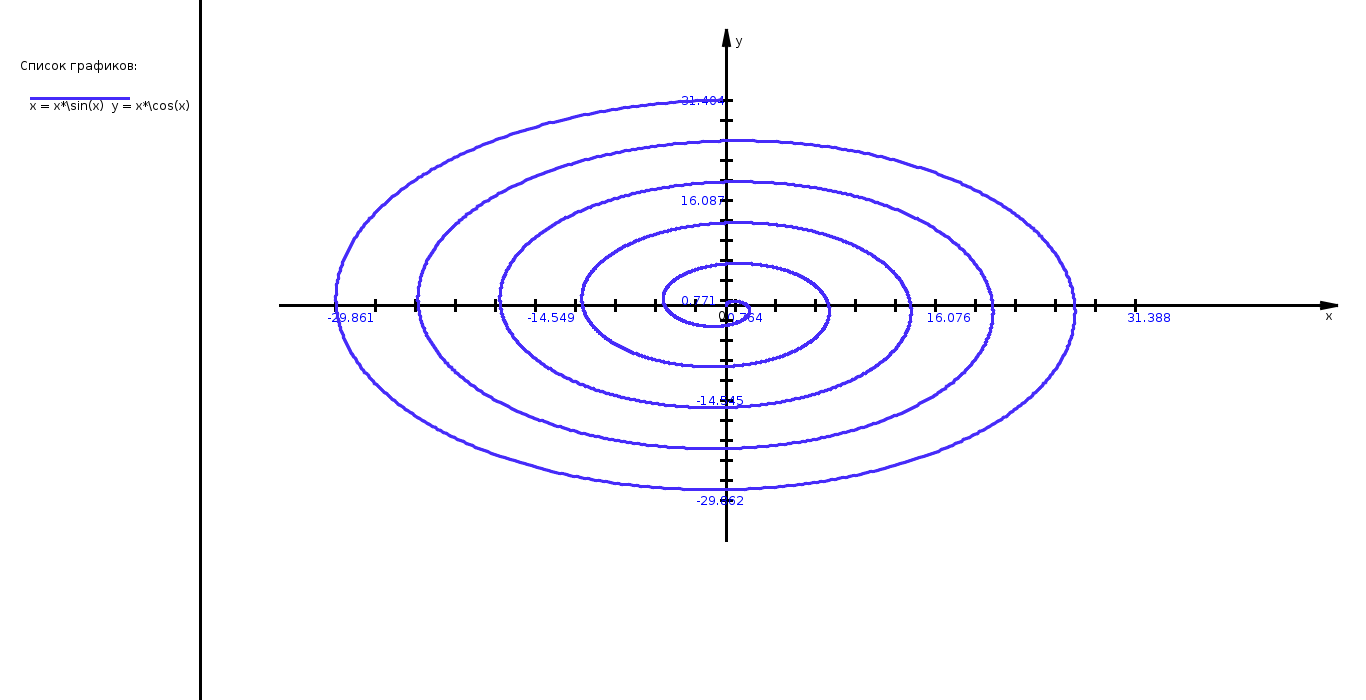
\includegraphics[scale=0.3]{pictures/2_2}
\vspace*{-10mm}
\caption{График функции, заданной параметрически}
\label{2_2}
\end{figure}



\underline{Пример 3. }

%enddelete

\vspace*{-2mm}
\begin{verbatim}
SPACE = R64[x, y, z];
g = 2\cos(x)+\cos(2x); 
k = 2\sin(x)-\sin(2x);
f = \paramPlot([g, k], [0, 2\pi]);
\end{verbatim}
\vspace*{-2mm}

%begindelete
\ex{$g=2\cos(x)+\cos(2x); k= 2\sin(x)-\sin(2x);$}{рис. \ref{2_3}.}
\begin{figure}[h!]
 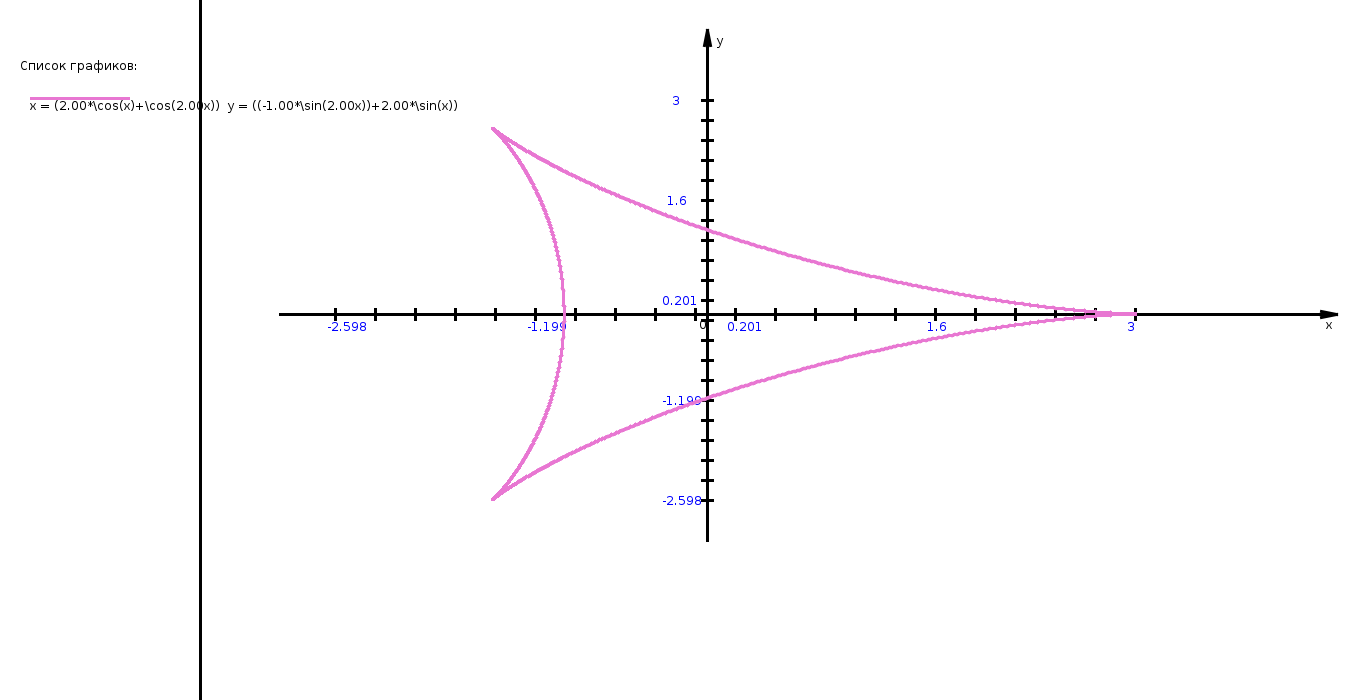
\includegraphics[scale=0.3]{pictures/2_3}
\vspace*{-10mm}
\caption{График функции, заданной параметрически}
\label{2_3}
\end{figure}

\eject
\underline{Пример 4. }


%enddelete

\vspace*{-2mm}
\begin{verbatim}
SPACE = R64[x, y, z];
g = 2\sin(x)^3; 
k = 2\cos(x)^3;
f = \paramPlot([g, k], [0, 2\pi]);
\end{verbatim}
\vspace*{-2mm}


%begindelete
\ex{$g=2\sin(x)^3; k= 2\cos^3(x)$}{рис. \ref{2_4}.}
\begin{figure}[h!]
 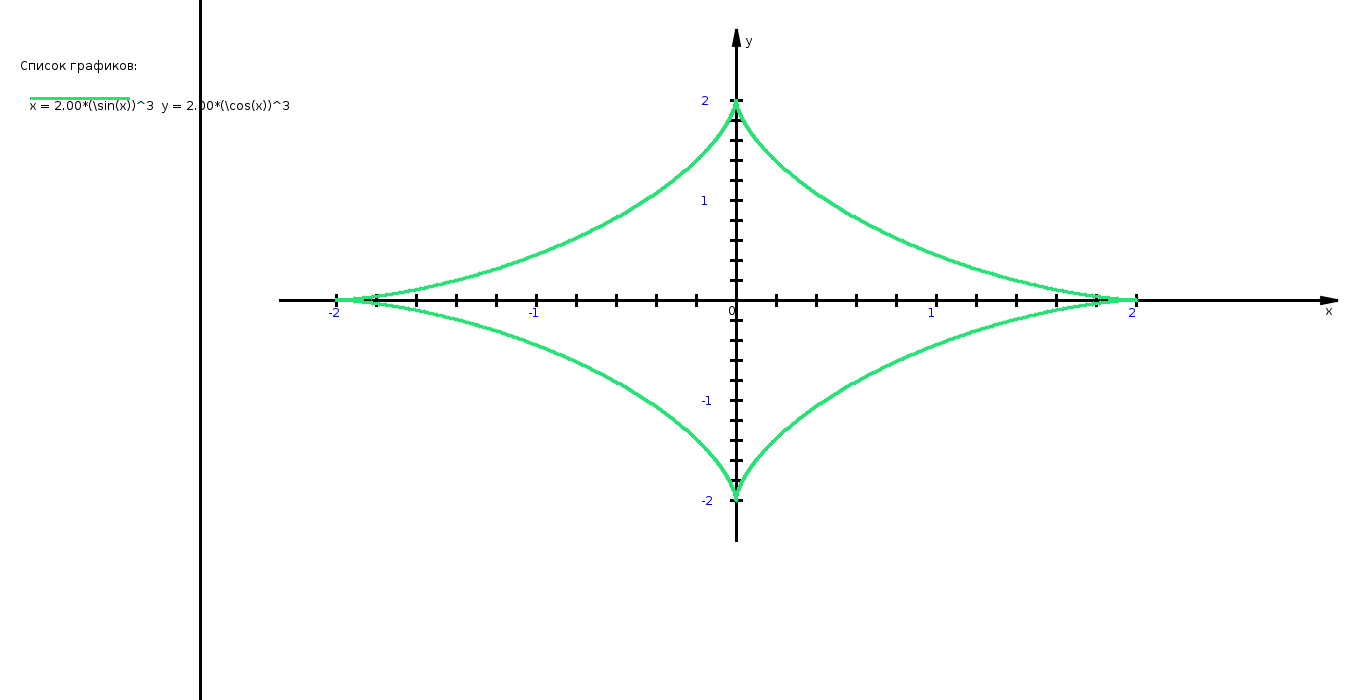
\includegraphics[scale=0.3]{pictures/2_4}
\vspace*{-10mm}
\caption{График функции, заданной параметрически}
\label{2_4}
\end{figure}



\underline{Пример 5. }
%enddelete

\vspace*{-2mm}
\begin{verbatim}
SPACE = R64[x, y, z];
g = (1+\cos(x))\cos(x); 
k = (1+\cos(x))\sin(x);
f = \paramPlot([g, k], [0, 2\pi]);
\end{verbatim}
\vspace*{-2mm}

%begindelete
\ex{$g=(1+\cos(x))\cos(x);k= (1+\cos(x))\sin(x);$}{рис. \ref{2_5}.}
\begin{figure}[h!]
 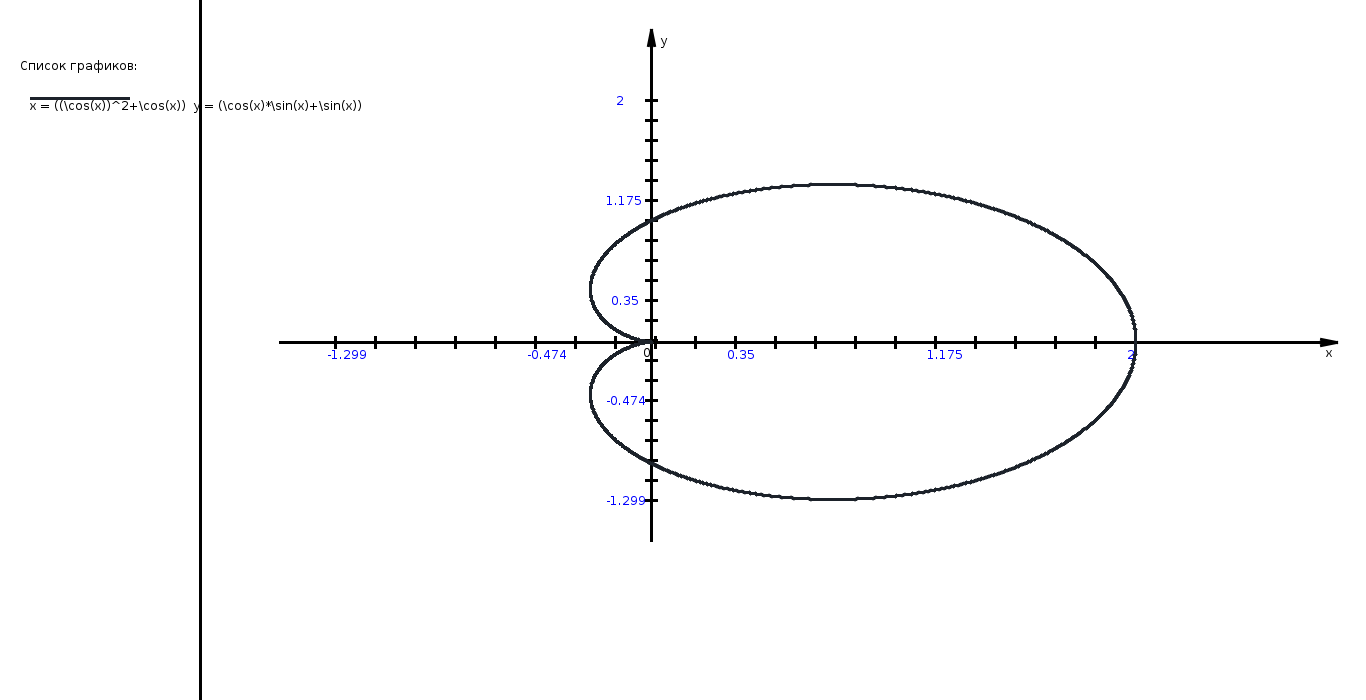
\includegraphics[scale=0.3]{pictures/2_5}
\vspace*{-10mm}
\caption{График функции, заданной параметрически}
\label{2_5}
\end{figure}

\eject
\underline{Пример 6. }
%enddelete


\vspace*{-2mm}
\begin{verbatim}
SPACE = R64[x, y, z];
g = \sin(x)(\exp(\cos(x))-2\cos(4x)+\sin(x/12)^5);
k = \cos(x)(\exp(\cos(x))-2\cos(4x)+\sin(x/12)^5);
f = \paramPlot([g, k], [0, 12\pi]);
\end{verbatim}
\vspace*{-2mm}


%begindelete
\ex{$g=\sin(x)(\exp(\cos(x))-2\cos(4x)+\sin^5(x/12));$\\
\hspace*{4mm} $k= \cos(x)(\exp(\cos(x))-2\cos(4x)+\sin^5(x/12));$}{рис. \ref{2_6}.}
\begin{figure}[h!]
 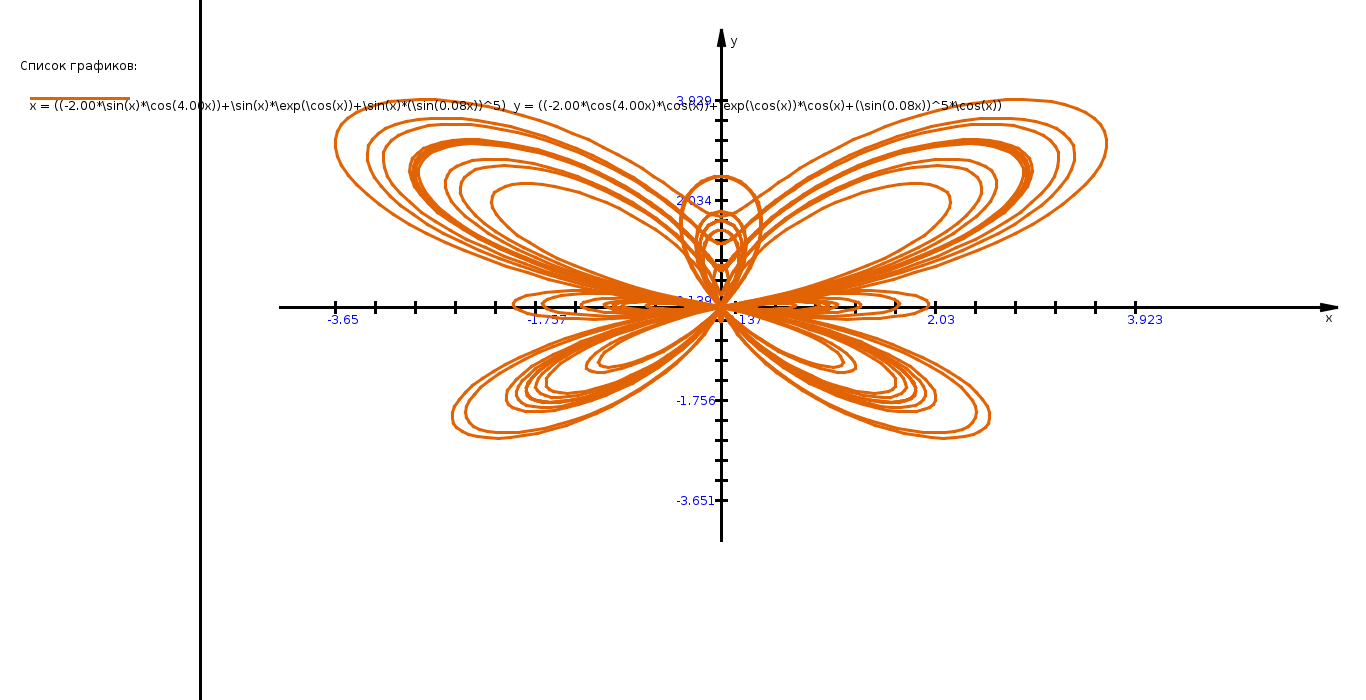
\includegraphics[scale=0.3]{pictures/2_6}
\vspace*{-10mm}
\caption{График функции, заданной параметрически}
\label{2_6}
\end{figure}
 

\eject
\underline{Пример 7. }
%enddelete


\vspace*{-2mm}
\begin{verbatim}
SPACE = R64[x, y, z];
\set2D('','','','','x(t)','y(t)','paramPlot');
g = \sin(x)(\exp(\cos(x))-2\cos(4x)+\sin(x/12)^5);
k = \cos(x)(\exp(\cos(x))-2\cos(4x)+\sin(x/12)^5);
f = \paramPlot([g, k], [0, 12\pi]);
\end{verbatim}
\vspace*{-2mm}

%begindelete
\eject
\underline{Пример 8. }
%enddelete

\vspace*{-2mm}
\begin{verbatim}
SPACE = R64[x, y, z];
g = \sin(x); 
k = \cos(x); 
f = \paramPlot([g, k], [0, 2\pi],'dashAndArrow');
\end{verbatim}
\vspace*{-2mm}


\subsection{Функции, которые заданы таблицей значений}

Для построения графиков функций, заданных табличными значениями, необходимо выполнить команду:
\comm{tablePlot}{([[x_{1},\ldots, x_{n}],[y_{11},\ldots,a_{1n}],\ldots,[y_{k1},\ldots,a_{kn}]])}
Другой вариант команды:
\comm{tablePlot}{([[x_{1},\ldots, x_{n}],[y_{11},\ldots,a_{1n}],\ldots,[y_{k1},\ldots,a_{kn}]], 'options')}
,где $'options'$~--- принимает следующие значения:\\
1)$'dash'$~--- график будет изображен пунктиром;\\ 
2)$'arrow'$~---  последняя точка графика будет нарисована со стрелкой;\\
3)$'dashAndArrow'$~--- график будет изображен пунктиром и последняя точка графика будет нарисована со стрелкой.

%begindelete
\underline{Пример 1.}
 
 \vspace*{-2mm}
%enddelete

 \begin{verbatim}
SPACE = R64[x, y, z];
 \tablePlot(
   [
     [0, 1, 2, 3, 4, 5],
     [0, 1, 4, 9, 16, 25],
     [0, -1, -2, -3, -4, -5],
     [0, 4, 8, 12, 16, 20]
   ]);
 \end{verbatim}

 %begindelete
\ex{}{рис. \ref{2_7}.}
\begin{figure}[!h]
 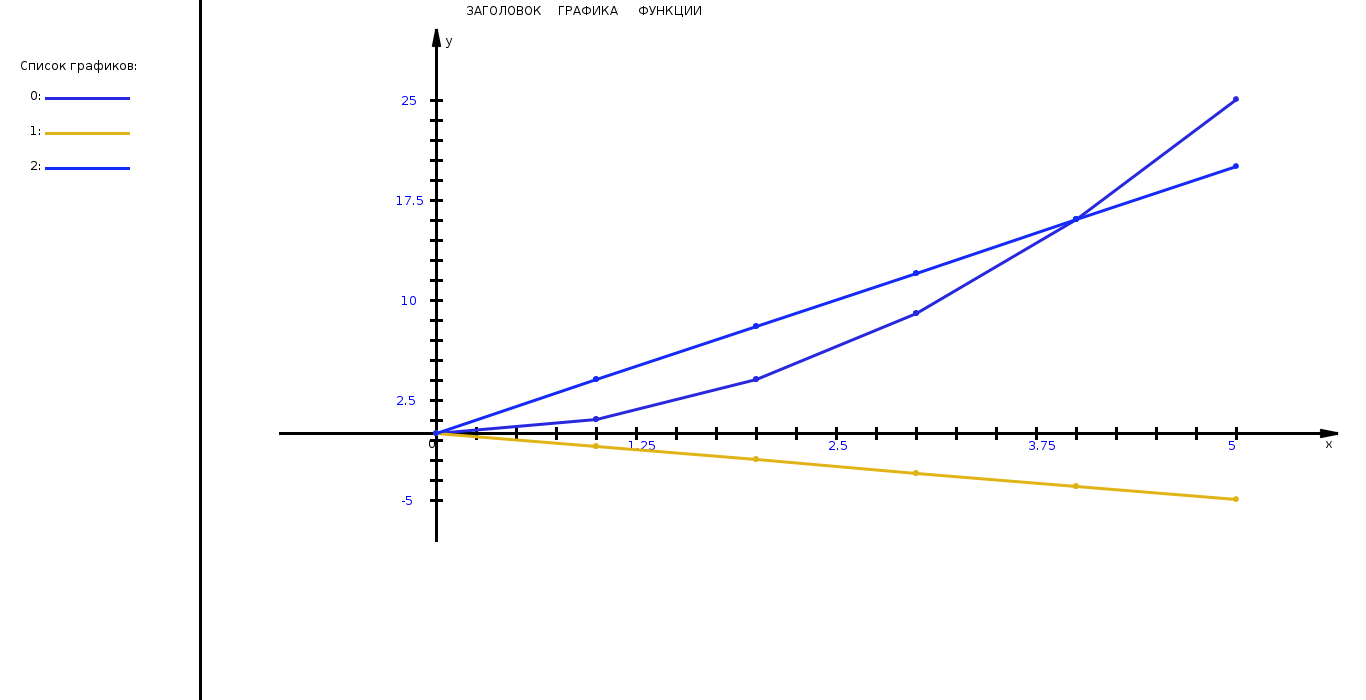
\includegraphics[scale=0.25]{pictures/2_7}
\vspace*{-10mm}
\caption{График функции, заданной таблицей значений}
\label{2_7}
\end{figure}


\underline{Пример 2.}
 %enddelete

 \vspace*{-2mm}
 \begin{verbatim}
SPACE=R64[x]; 
\set2D(-1,5,-10,10);
"Пусть задана табличная функция:" 
A=[[0, 1, 2, 3,  4, 5],    [3, 0, 4, 10, 5, 10]]; t=\table(A);
"Аппроксимируем эту функцию полиномом 4-й степени:" p=\approx(t,4);
"Построим график полинома:" P=\plot(p,[1,5]);
"Построим график табличной функции:" T=\tablePlot(t);
"Построим оба графика в одной системе координат:" \showPlots([P,T]);
\print(p);
 \end{verbatim}

%begindelete
\ex{}{$0.54x^4-5.64x^3+18.38x^2-17.28x+3.17$\\
\hspace*{4mm} рис. \ref{2_8}.}
\begin{figure}[!h]
 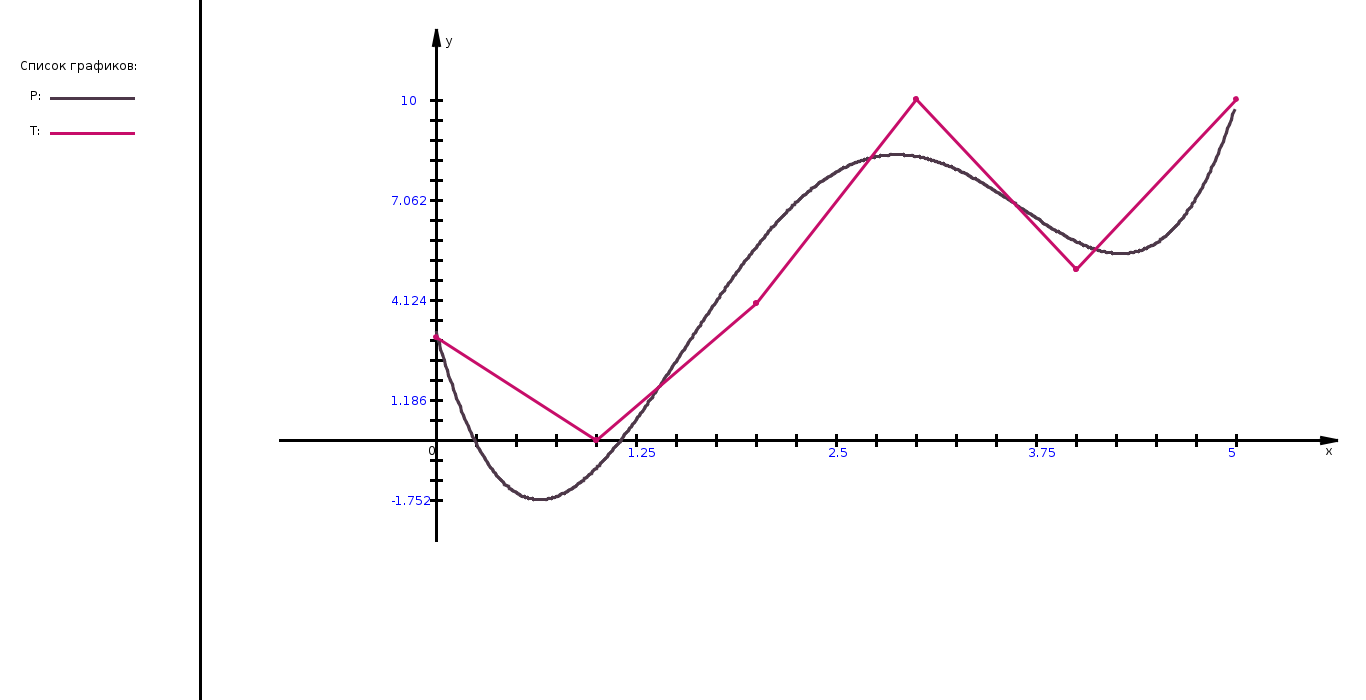
\includegraphics[scale=0.25]{pictures/2_8}
\vspace*{-10mm}
\caption{График аппроксимации функции, заданной таблицей значений}
\label{2_8}
\end{figure}
%enddelete

%begindelete
\underline{Пример 3.}
 
 \vspace*{-2mm}
%enddelete

 \begin{verbatim}
SPACE = R64[x, y, z];
\set2D(-10, 10, -10, 10, '','', 'Header of Graphics');
 \tablePlot(
   [[-3, -6, -6, -3, 3, 6, 6, 3, -3],
    [6, 3, -3, -6, -6, -3, 3, 6, 6]]);
 \end{verbatim}

%begindelete
\underline{Пример 4.}
 
 \vspace*{-2mm}
%enddelete

 \begin{verbatim}
SPACE = R64[x, y, z];
 \tablePlot(
   [[-3, -6, -6, -3, 3, 6, 6, 3, -3],
    [6, 3, -3, -6, -6, -3, 3, 6, 6]],'arrow');
 \end{verbatim}

%begindelete
\underline{Пример 5.}
 
 \vspace*{-2mm}
%enddelete

 \begin{verbatim}
SPACE = R64[x, y, z];
 \tablePlot(
   [[-3, -6, -6, -3, 3, 6, 6, 3, -3],
    [6, 3, -3, -6, -6, -3, 3, 6, 6]], 'dash');
 \end{verbatim}

%begindelete
\underline{Пример 6.}
 
 \vspace*{-2mm}
%enddelete

 \begin{verbatim}
SPACE = R64[x, y, z];
 \tablePlot(
   [[-3, -6, -6, -3, 3, 6, 6, 3, -3],
    [6, 3, -3, -6, -6, -3, 3, 6, 6]], 'dashAndArrow');
 \end{verbatim}

\subsection{Функции, которые заданы таблицей значений по точкам}
Для построения графиков функций по точкам, заданных табличными значениями, необходимо выполнить команду: 
\comm{pointsPlot}{([[x_{1},\ldots, x_{n}],[y_{1},\ldots,y_{n}]], [s_{1},\ldots,s_{n}], [kv_{1},\ldots,kv_{n}], [kg_{1},\ldots,kg_{n}])},\\
где $s_{n}$~--- подпись точки, $kv_{n}$~--- коэффициент поворота вокруг точки (принимает значения от 0 до 7, и означает поворот на ($kv_{n}$ * 45) градусов), 
$kg_{n}$~--- коэффициент смещения вдоль оси $OX$ (если отрицательный то смещение происходит влево).
Сокращенные варианты команды:
\comm{pointsPlot}{([[x_{1},\ldots, x_{n}],[y_{1},\ldots,y_{n}]], [s_{1},\ldots,s_{n}])}
или
\comm{pointsPlot}{([[x_{1},\ldots, x_{n}],[y_{1},\ldots,y_{n}]], [s_{1},\ldots,s_{n}], [kv_{1},\ldots,kv_{n}])}
или
\comm{pointsPlot}{([[x_{1},\ldots, x_{n}],[y_{1},\ldots,y_{n}]], [s_{1},\ldots,s_{n}], [kv_{1},\ldots,kv_{n}], [kg_{1},\ldots,kg_{n}])}.

%begindelete
\underline{Пример 1.}
 
 \vspace*{-2mm}
%enddelete

 \begin{verbatim}
\set2D(-10, 10, -10, 10);
\pointsPlot(
   [[0, 1, 2],
     [0, 1, 4]],['a','b','c']);
 \end{verbatim}

%begindelete
\underline{Пример 2.}
 
 \vspace*{-2mm}
%enddelete

 \begin{verbatim}
 \pointsPlot(
   [
     [0, 1, 2],
     [0, 1, 4]],['a','b','c'],[0,2,4]);
 \end{verbatim}

%begindelete
\underline{Пример 3.}
 
 \vspace*{-2mm}
%enddelete

 \begin{verbatim}
 \pointsPlot(
   [
     [0, 1, 2],
     [0, 1, 4]],['a','b','c'],[0,2,4],[0,-5,5]);
 \end{verbatim}

%begindelete
\underline{Пример 4.}
 
 \vspace*{-2mm}
%enddelete

 \begin{verbatim}
 \pointsPlot(
   [
     [0, 1, 2],
     [0, 1, 4]]);
 \end{verbatim}

%begindelete
\underline{Пример 5.}
 
 \vspace*{-2mm}
%enddelete

 \begin{verbatim}
SPACE = R64[x, y, z];
f1=\tablePlot([[1, 1], [1, 5]]);
f2=\tablePlot([[1, 5], [1, 1]]);
f3=\tablePlot([[5, 5], [1, 5]]);
f4=\tablePlot([[1, 5], [5, 5]]);
f5=\pointsPlot([[1, 1, 5, 5],[1, 5, 5, 1]],['A','B','C','D'],[6,0,0,2]);
\showPlots([f1, f2, f3, f4, f5]);
 \end{verbatim}

%begindelete
\underline{Пример 6.}
 
 \vspace*{-2mm}
%enddelete

 \begin{verbatim}
SPACE = R64[x, y, z];
f1=\tablePlot([[1, 1], [1, 5]]);
f2=\tablePlot([[1, 5], [1, 1]]);
f3=\tablePlot([[5, 5], [1, 5]]);
f4=\tablePlot([[1, 5], [5, 5]]);
f5=\pointsPlot([[1, 1, 5, 5],[1, 5, 5, 1]],['A','B','C','D'],[6,0,0,2]);
\showPlots([f1, f2, f3, f4, f5],'noAxes');
 \end{verbatim}

\subsection{Построение разных графиков функций в одной системе координат}
Для построения графиков функций,  заданных разными способами,  необходимо сначала построить график каждой функции,  а затем выполнить команду
\comm{showPlots}{([f_1, f_2, \ldots, f_n])}.
Другие варианты команды:
\comm{showPlots}{([f1, f2, f3, f4], 'noAxes')}, где 'noAxes'~--- параметр, указывающий на изображение графика без осей.
или
\comm{showPlots}{([f1, f2, f3, f4], 'lattice')}, где 'lattice'~--- параметр, указывающий на изображение графика c решеткой.

%begindelete
\underline{Пример 1.}
 
 \vspace*{-2mm}
%enddelete

\begin{verbatim}
SPACE = R64[x, y, z];
\set2D(-20, 20, -20, 20);
f1 = \plot(\tg(x));
f2 = \tablePlot([[0, 1, 4, 9, 16, 25], [0, 1, 2, 3, 4, 5]]);
f3 = \paramPlot([\sin(x), \cos(x)], [-10, 10]);
f4=\tablePlot([[0, 1, 4, 9, 16, 25], [0, -1, -2, -3, -4, -5]]);
\showPlots([f1, f2, f3, f4]);
\end{verbatim}
%begindelete
\ex{}{рис. \ref{3_6}.}
\begin{figure}[!ht]
 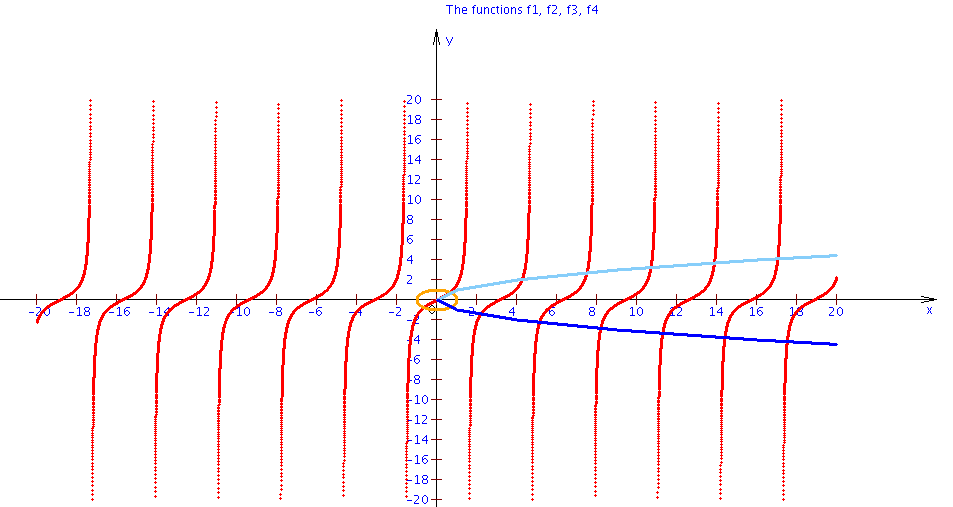
\includegraphics[scale=0.6]{pictures/3_6}
\caption{Графики функций,  заданных разными способами}
\label{3_6}
\end{figure}
%enddelete

%begindelete
\underline{Пример 2.}
 
 \vspace*{-2mm}
%enddelete

 \begin{verbatim}
p1=\tablePlot([[-1, -3, 3, 3, -3, -3],[4, 3, 3, -3 , -3, 3]]);
p2=\tablePlot([[5, 5, 3, 3, 5, -1],[4, -2, -3, 3, 4, 4]]);
p3=\tablePlot([[-3, -1, -1],[-3, -2, 4]], 'dash');
p4=\tablePlot([[-1, 5],[-2, -2]], 'dash');
\showPlots([p1,p2,p3,p4], 'noAxes');
 \end{verbatim}

%begindelete
\underline{Пример 3.}
 
 \vspace*{-2mm}
%enddelete

 \begin{verbatim}
p1=\tablePlot([[-1, -3, 3, 3, -3, -3],[4, 3, 3, -3, -3, 3]]);
p1p=\pointsPlot([[-1, -3, 3, 3, -3],[4, 3, 3, -3 , -3]],
['F','B','C','D','A'],[0,0,0,4,4]);
p2=\tablePlot([[5, 5, 3, 3, 5, -1],[4, -2, -3, 3, 4, 4]]);
p3=\tablePlot([[-3, -1, -1],[-3, -2, 4]],'dash');
p4=\tablePlot([[-1, 5],[-2, -2]],'dash');
p2p=\pointsPlot([[5, 5, -1 ],[4, -2, -2]],['G','H','E'],[0,4,4]);
\showPlots([p1,p2,p3,p4,p1p,p2p], 'noAxes');
 \end{verbatim}


\subsection{Построение графов}
Для построения графов необходимо выполнить команду 
\comm{plotGraph}{([[a_{11},\ldots,a_{1n}],\ldots,[a_{n1},\ldots,a_{nn}]], [[x_{1},\ldots, x_{n}],[y_{1},\ldots,y_{n}]])}, 
где $[[a_{11},\ldots,a_{1n}],\ldots,[a_{n1},\ldots,a_{nn}]]$~--- матрица смежности, $[[x_{1},\ldots, x_{n}],[y_{1},\ldots,y_{n}]]$~--- матрица координат.

%begindelete
\underline{Пример 1. }

\vspace*{-2mm}
%enddelete
\begin{verbatim}
\plotGraph([[0,1,1,0,1,0],[1,0,0,1,1,0],[1,0,0,0,1,1],[0,1,0,0,0,0],
[1,1,1,0,0,1],[0,0,1,0,1,0]],[[3,2,4,1,3,5],[3,2,2,1,1,1]]);
\end{verbatim}
%begindelete
\ex{}{рис. \ref{4_1}.}
\begin{figure}[!ht]
 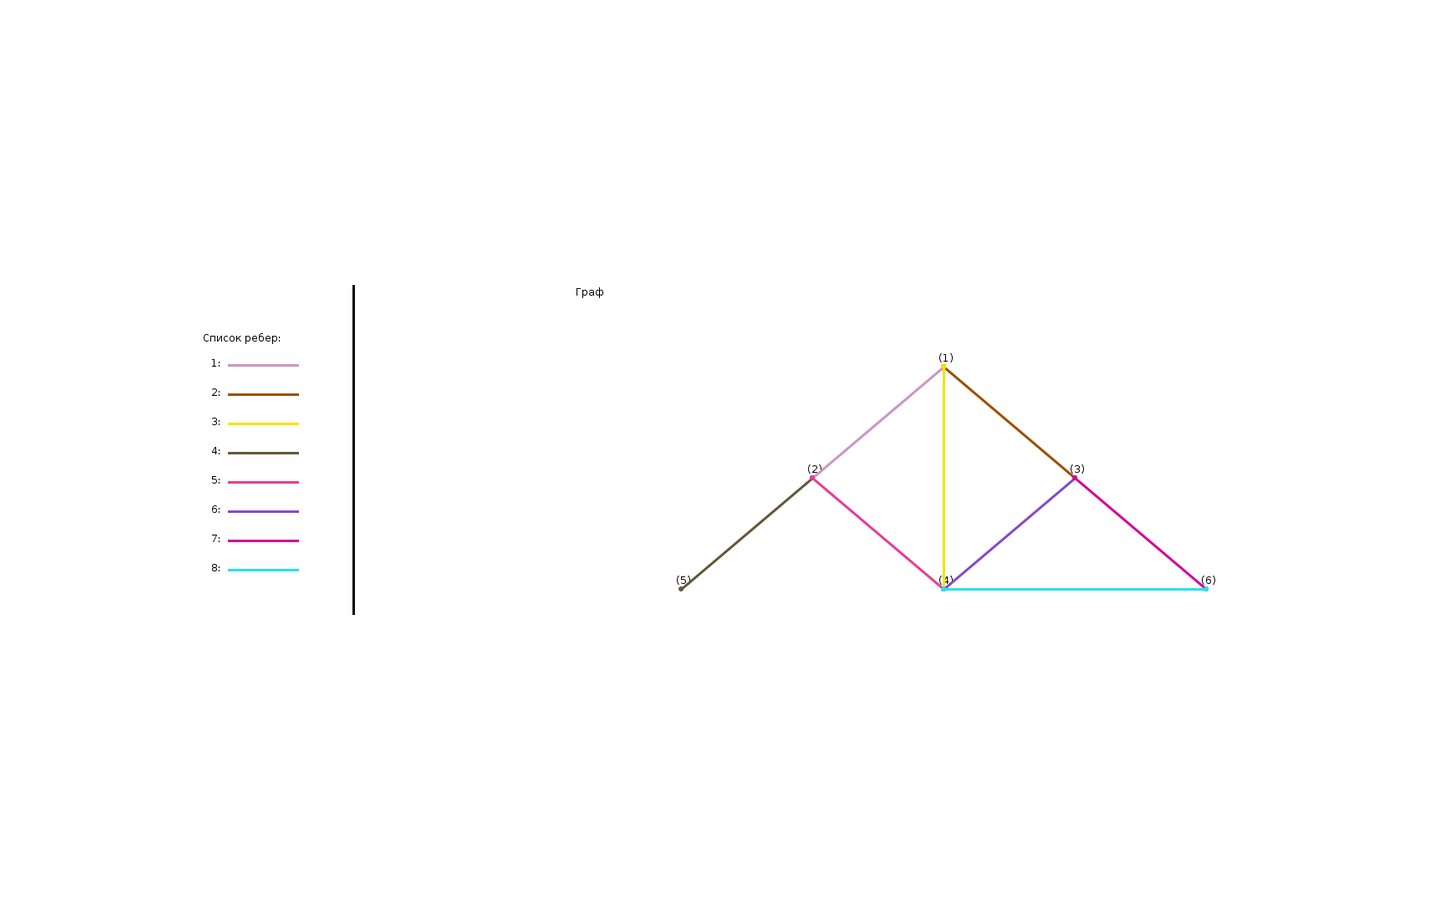
\includegraphics[scale=0.4]{pictures/4_1}
\caption{Граф}
\label{4_1}
\end{figure}
%enddelete

Кроме того, можно выполнить команду лишь с первым параметром 
\comm{plotGraph}{([[a_{11},\ldots,a_{1n}],\ldots,[a_{n1},\ldots,a_{nn}]])}, 
где $[[a_{11},\ldots,a_{1n}],\ldots,[a_{n1},\ldots,a_{nn}]]$~--- матрица смежности.

%begindelete
\underline{Пример 2. }

\vspace*{-2mm}%enddelete
\begin{verbatim}
\plotGraph([[0,1,1,0,1,0],[1,0,0,1,1,0],[1,0,0,0,1,1],[0,1,0,0,0,0],
[1,1,1,0,0,1],[0,0,1,0,1,0]]);
\end{verbatim}
%begindelete
\ex{}{рис. \ref{4_2}.}
\begin{figure}[!ht]
 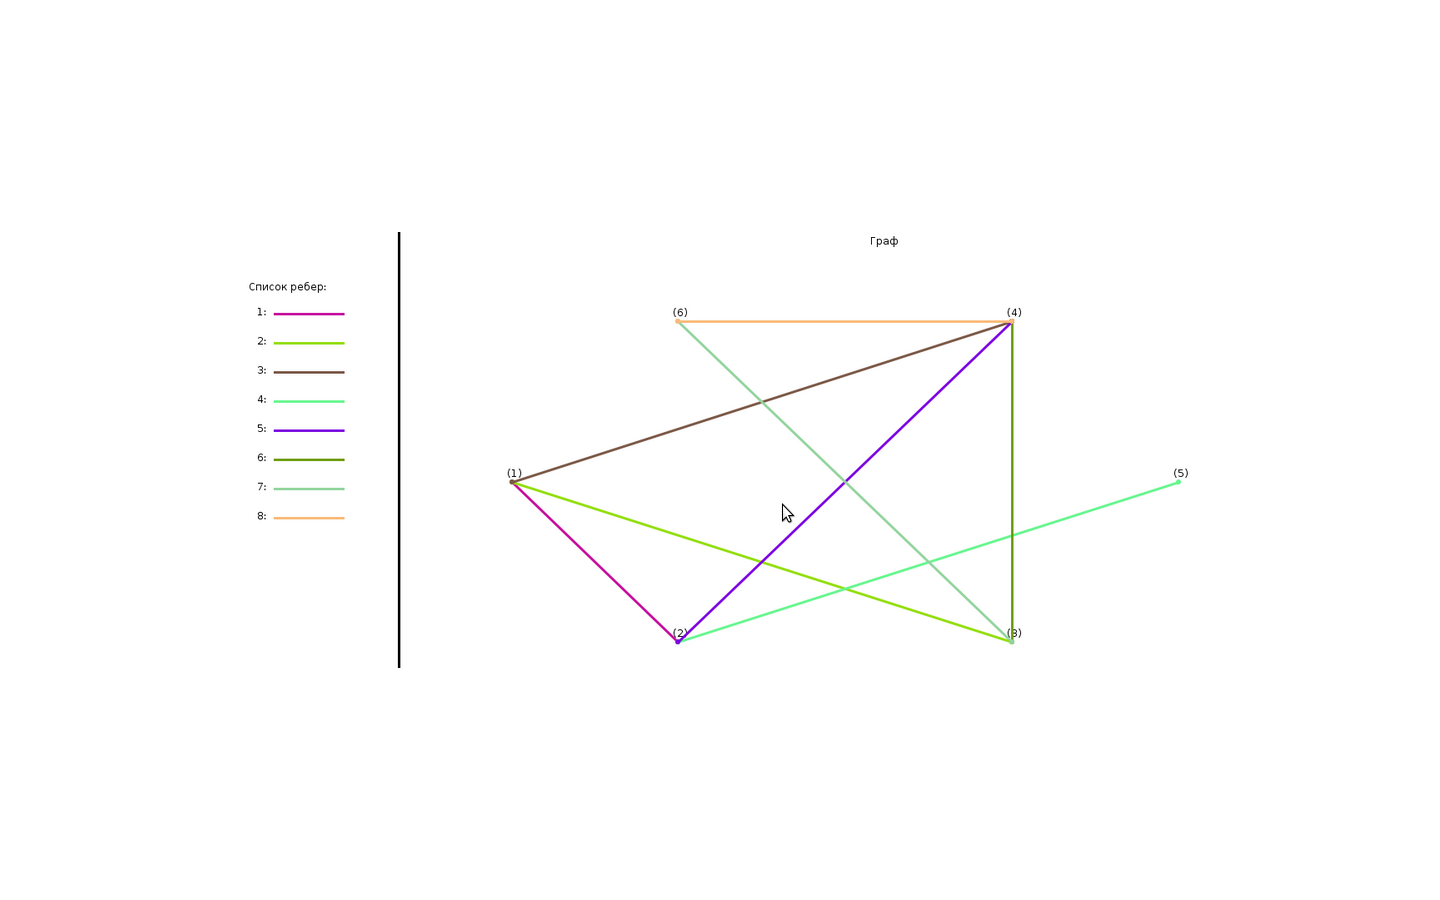
\includegraphics[scale=0.4]{pictures/4_2}
\caption{Граф}
\label{4_2}
\end{figure}
%enddelete

Можно выполнить команду с одним числовым параметром 
\comm{plotGraph}{(N)}, 
где $N$~--- количество вершин в графе.

%begindelete
\underline{Пример 3. }

\vspace*{-2mm}%enddelete
\begin{verbatim}
\plotGraph(6);
\end{verbatim}
%begindelete
\ex{}{рис. \ref{4_3}.}
\begin{figure}[!ht]
 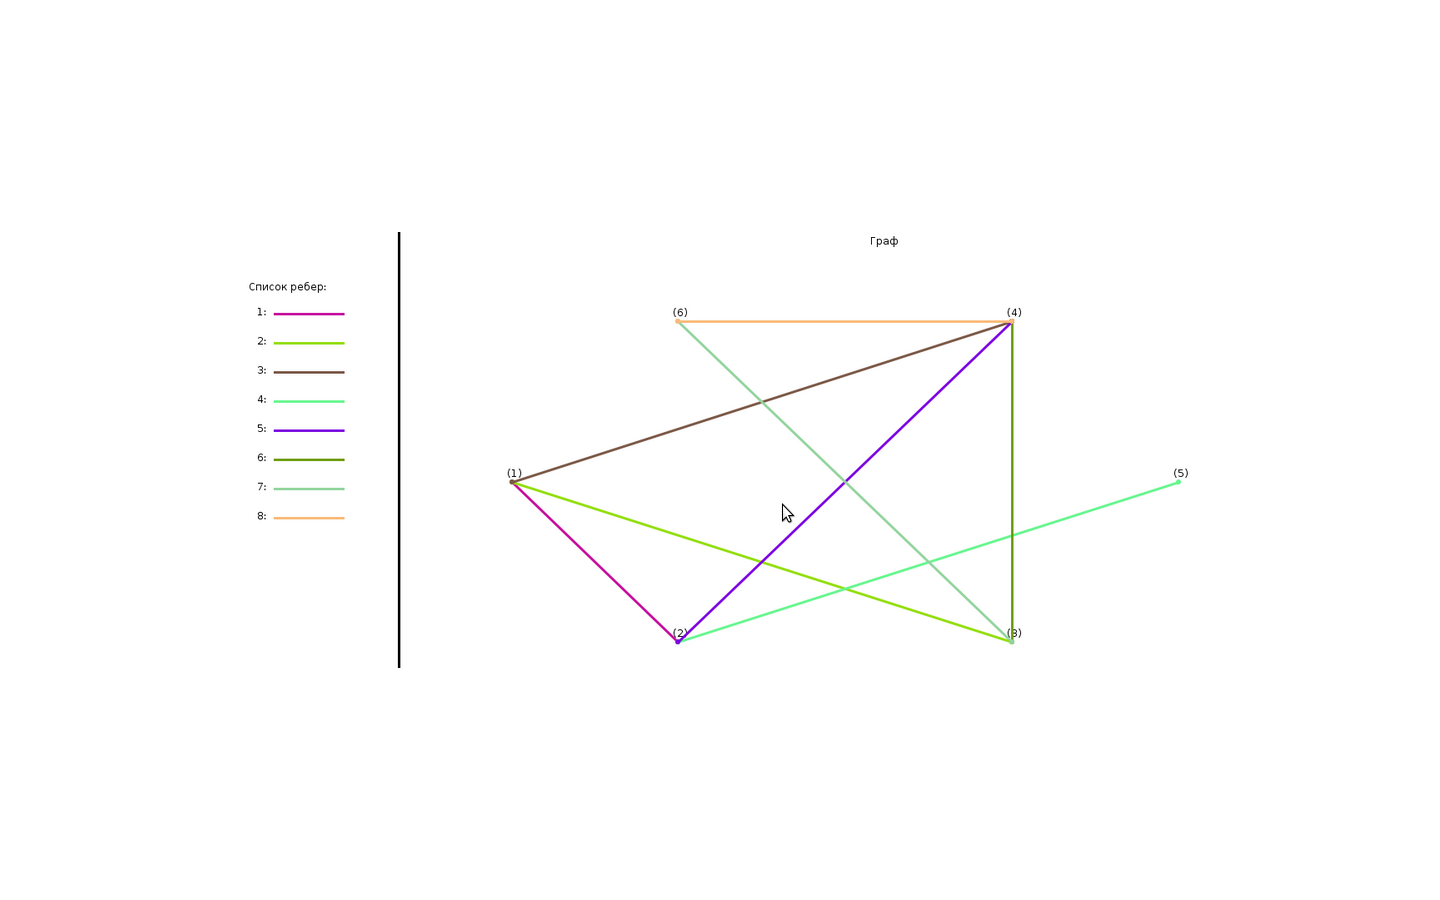
\includegraphics[scale=0.4]{pictures/4_2}
\caption{Граф}
\label{4_3}
\end{figure}
%enddelete


\subsection{Текст на графиках}
Для того, чтобы делать любые виды надписей используется функция
\comm{textPlot}{()}

Для задания одной надписи записывают в кваратных скобках
следуюшие параметры: ['str',sizeText,xCor,yCor,alpha]

  где str - это текст; sizeText - размер шрифта; xCor, yCor - координаты на экране первой буквы текста,
  alpha - угол наклона текста  (по умолчанию, если это параметр не указан, то он равен нулю). 

В одной команде можно определить сколько угоно надписей, разделяя их запятыми:\\
  \comm{textPlot}{([],[],[],...[])}.

\section{Построение 3D графиков функций}
 Mathpar позволяет строить 3D графики функций, которые заданы явно. 
 
 Для построения 3D графика функции $f=f(x, y)$ используется команда 
\comm{plot3d}{(f, [x0, x1, y0, y1])},
 где $[x0, x1]$~--- интервал по оси $OX$,  $[y0, y1]$~--- интервал по оси $OY$. 
 
Кроме того,  полученные графики можно вращать и масштабировать: увеличивать либо уменьшать. 

 Перемещение мыши с нажатой левой кнопкой приводит к вращению системы координат графика. 
 После остановки происходит перерисовка графика в новой повернутой системе координат. 
 
 Перемещение мыши с нажатой левой кнопкой и нажатой клавишей {\it Shift} приводит к изменению масштаба изображения. 
 После остановки перемещения происходит перерисовка графика в новом масштабе.  

\underline{Пример. }

\vspace*{-2mm}

\begin{verbatim}
f = x^2 / 20 + y^2 / 20;
\plot3d(f, [-20, 20, -20, 20]);
\end{verbatim}

\begin{verbatim}
\plot3d([x / 20 + y^2 / 20, x^2 / 20 + y / 20], [-20, 20, -20, 20]);
\end{verbatim}

\begin{verbatim}
SPACE = R64[x, y, a, b];
f = ax^2 / 20 + by^2 / 20;
\plot3d(f, [-20, 20, -20, 20]);
\end{verbatim}

%begindelete

Для построения графика функции во времени с изменением параметров необходимо указать количество кадров - (например установим: frames = 5) (см. Рис.1.)

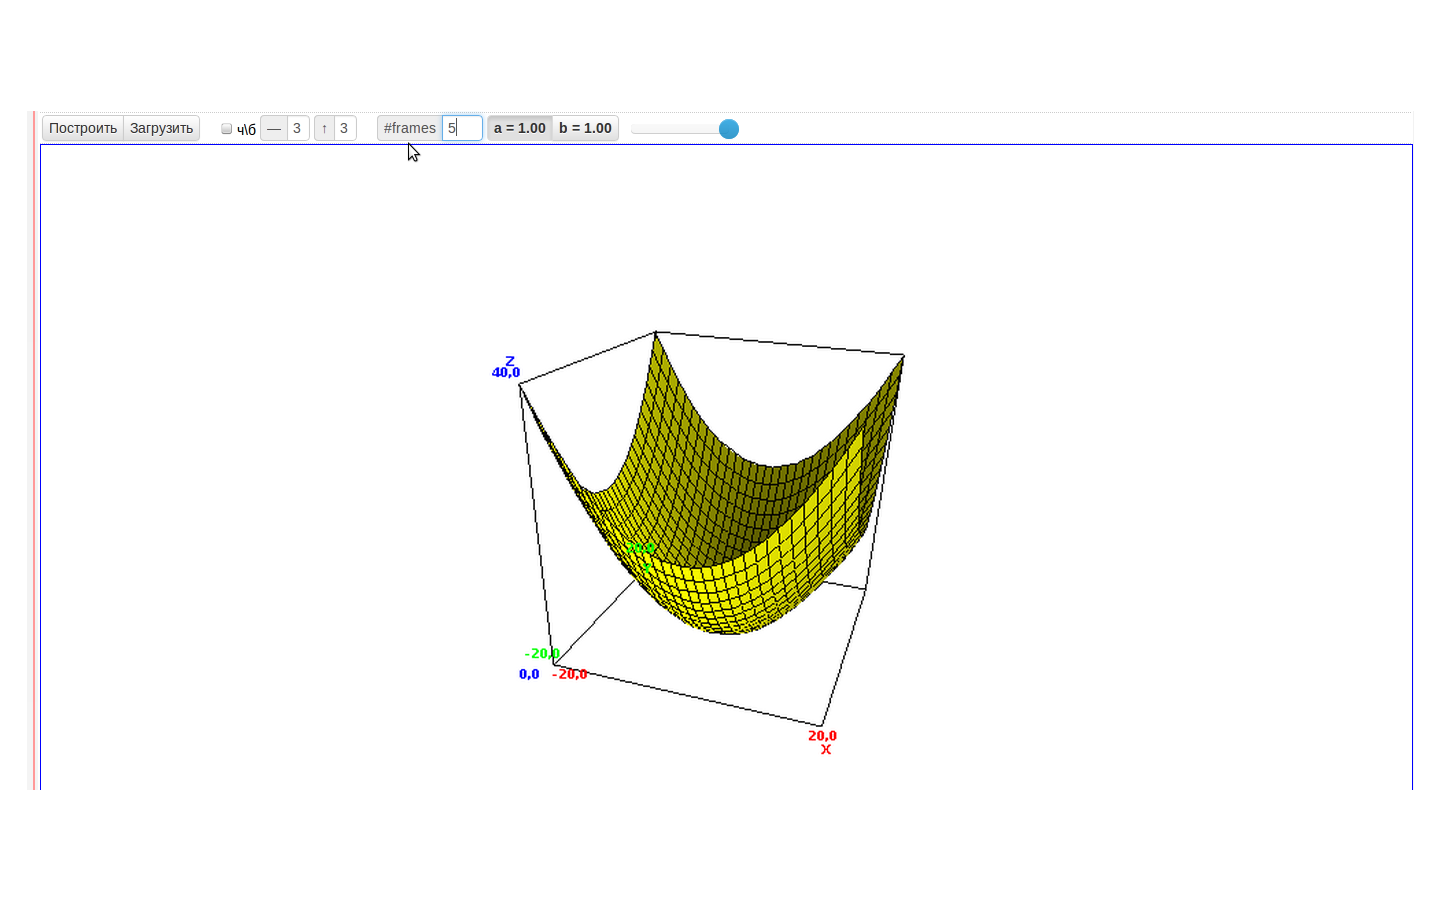
\includegraphics[scale=0.35]{pictures/3_9}
Рис. 1.

Для изменения параметров используйте ползунок - (например установим: a = 0.7, b = 0.24) (см. Рис.2.)

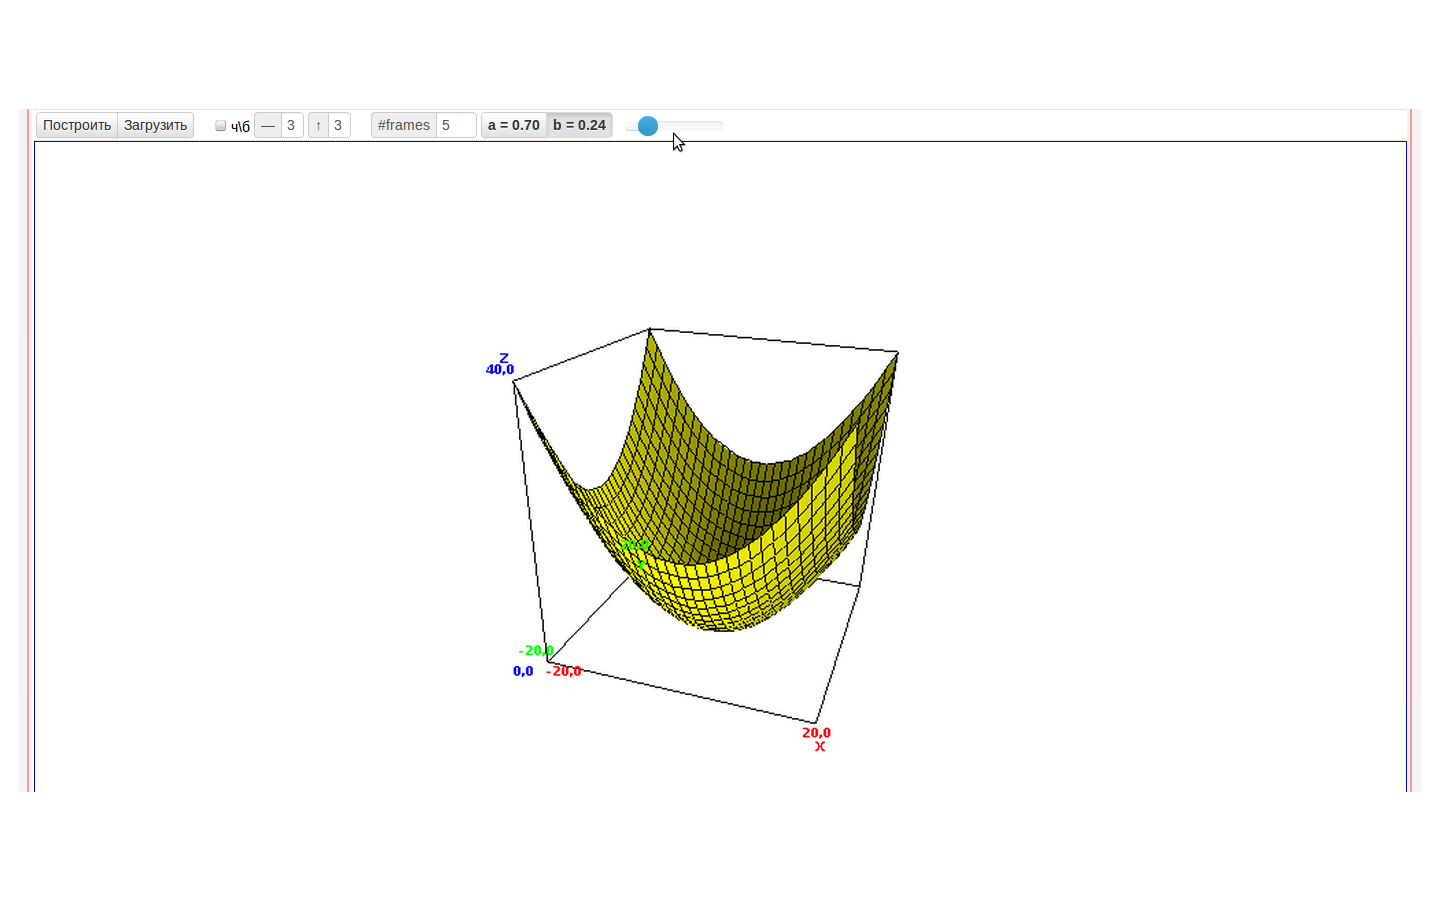
\includegraphics[scale=0.35]{pictures/3_10}
Рис. 2.

Для построения графика нажимаем кнопку - 'Построить' (см. Рис.3.)

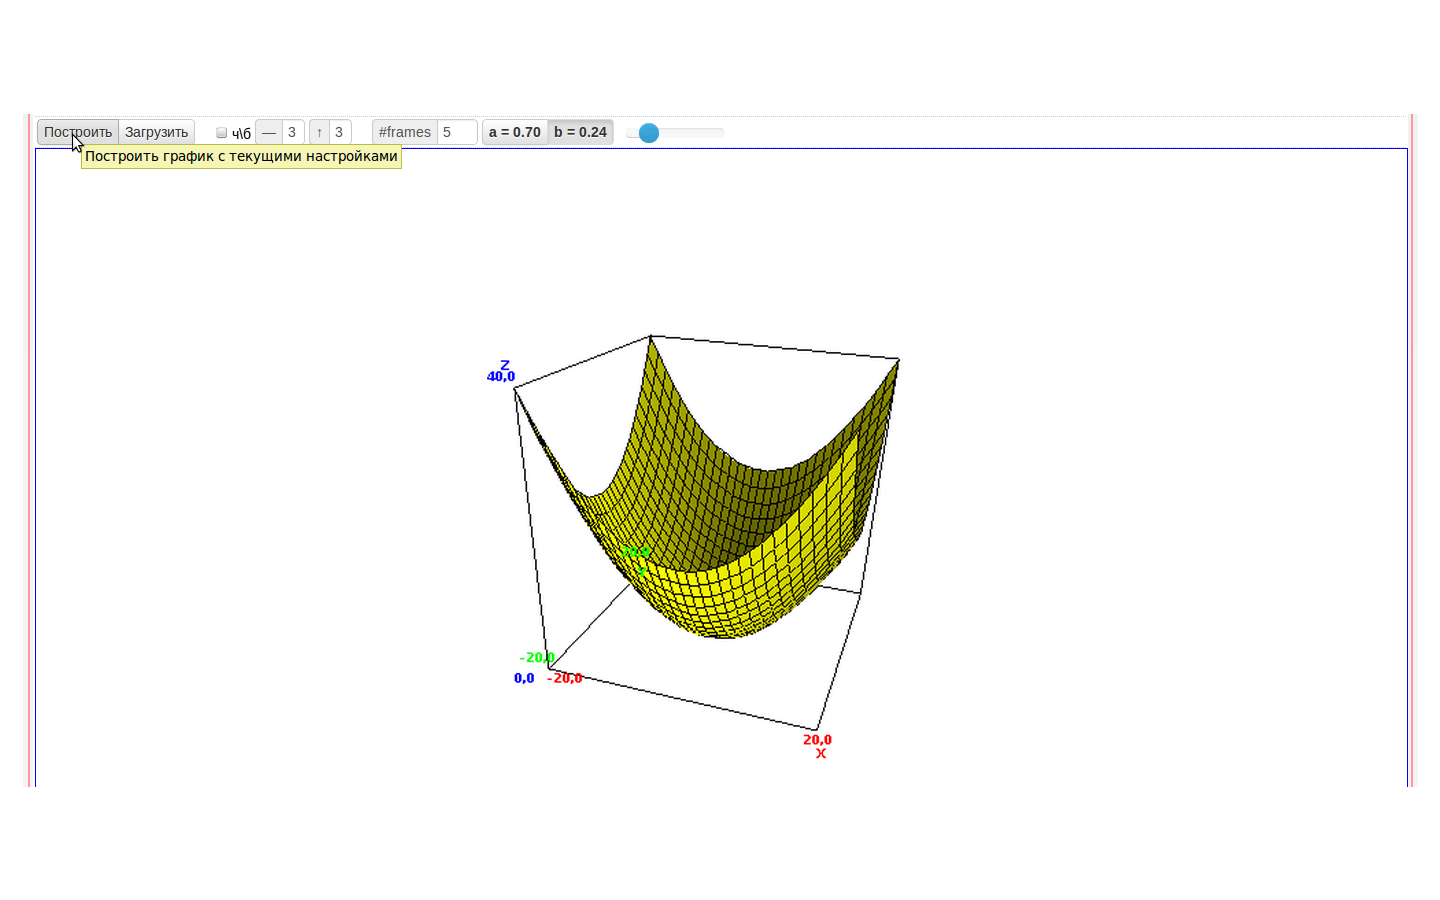
\includegraphics[scale=0.35]{pictures/3_11}
Рис. 3.

В результате получаем график.(см. Рис.4.)

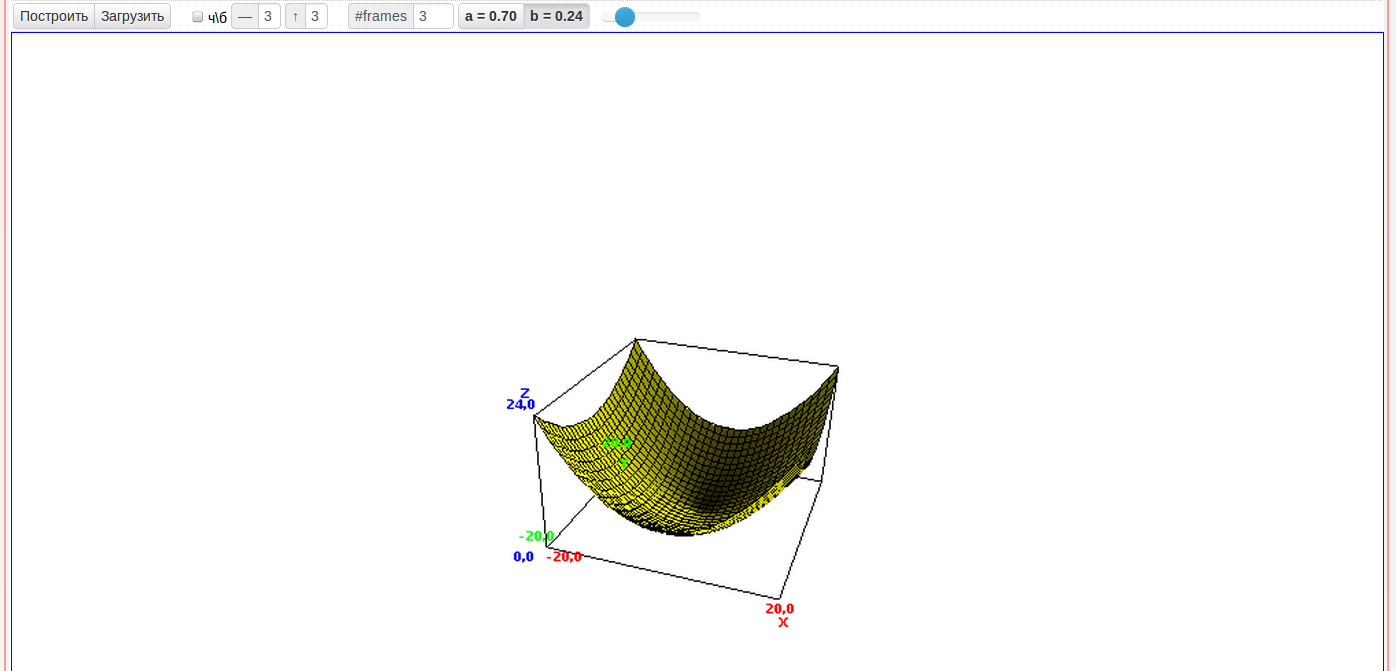
\includegraphics[scale=0.35]{pictures/3_12}
Рис. 4.

%enddelete

%begindelete
 
\ex{$f=x^2/20+y^2/20;$\\
\hspace*{4mm} $plot3d(f, [-20, 20, -20, 20]);$\\
\hspace*{4mm} $plot3d([x/20+y^2/20, x^2/20+y/20], [-20, 20, -20, 20]);$}
{рис. \ref{3_7}.}

\begin{figure}[!ht]
  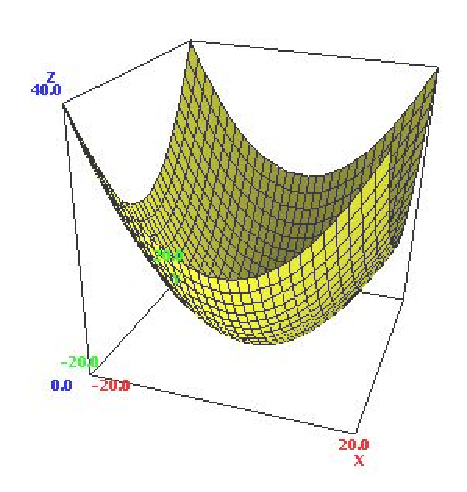
\includegraphics[width=138pt, height=146pt]{pictures/3_7}
  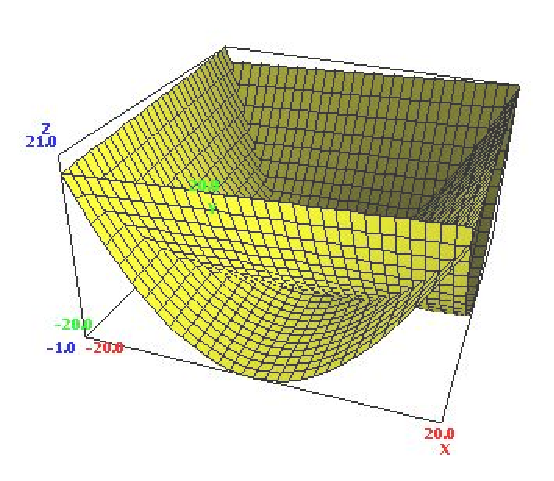
\includegraphics[width=166.5pt, height=143pt]{pictures/3_8}
  \caption{Построение 3D графиков функций}
  \label{3_7}
\end{figure}
%enddelete

Сфера

\begin{verbatim}
SPACE=R64[u,v];
\paramPlot3d([[\cos(u)\cos(v)], [\sin(u)\cos(v)], [\sin(v)]], 
[-\pi, \pi, -\pi/2, \pi/2]);
\end{verbatim}

Тор

\begin{verbatim}
SPACE=R64[u,v];
\paramPlot3d([[\cos(u)(\cos(v)+3)],[\sin(u)(\cos(v)+3)],[\sin(v)]], 
[-\pi, \pi, -\pi, \pi]);
\end{verbatim}

Спираль

\begin{verbatim}
SPACE=R64[u,v];
\paramPlot3d([[\cos(u)(\cos(v)+3)],[\sin(u)(\cos(v)+3)],[\sin(v)+u]], 
[-2\pi, 2\pi, -\pi, \pi]);
\end{verbatim}

Логарифмическая спираль

\begin{verbatim}
SPACE=R64[u,v];
\paramPlot3d([[u\cos(u)(\cos(v)+1)],[u\sin(u)(\cos(v)+1)],[u\sin(v)]], 
[0, 3\pi, -\pi, \pi]);
\end{verbatim}

"Морская раковина"

\begin{verbatim}
SPACE=R64[u,v];
\paramPlot3d([[u\cos(u)(\cos(v)+1)],[u\sin(u)(\cos(v)+1)],
[u\sin(v)-(((u+3)/8)\pi)^2-20]], [0, 8\pi, -\pi, \pi]);
\end{verbatim}

Трилистник

\begin{verbatim}
SPACE=R64[u,v];
\paramPlot3d([[\cos(u)\cos(v)+3\cos(u)(1.5+\sin(1.5u/2))],
[\sin(u)\cos(v)+3\sin(u)(1.5+\sin(1.5u/2))],[\sin(v)+2\cos(1.5u)]], 
[-2\pi, 2\pi, -\pi, \pi]);
\end{verbatim}

Поверхность Дини

\begin{verbatim}
SPACE=R64[u,v];
\paramPlot3d([[\cos(u)\sin(v)],[\sin(u)\sin(v)],
[\cos(v)+\lg(\tg(v/2))+0.2u-4]], [0, 4\pi, 0.0001, 2]);
\end{verbatim}

Лента Мёбиуса

\begin{verbatim}
SPACE=R64[u,v];
\paramPlot3d([[(1+v/2\cos(u/2))\cos(u)],[(1+v/2\cos(u/2))\sin(u)],
[v/2\sin(u/2)]], [0, 2\pi, -1, 1]);
\end{verbatim}

Куб

\begin{verbatim}
SPACE=R64[u,v];
\paramPlot3d([[u,v,5,u,v,-5],[v,5,u,v,-5,u],[5,u,v,-5,u,v]], 
[-5, 5, -5, 5]);
\end{verbatim}

Цилиндр

\begin{verbatim}
SPACE=R64[u,v];
\paramPlot3d([[5\cos(u)],[5\sin(u)],[v]], [-5, 5, -5, 5]);
\end{verbatim}

Конус

\begin{verbatim}
SPACE=R64[u,v];
\paramPlot3d([[\cos(u) * (5 * (1 - v/6))],[\sin(u) * (5 * (1 - v/6))],[v]], 
[-6, 6, 0, 6]);
\end{verbatim}

Усеченный конус

\begin{verbatim}
SPACE=R64[u,v];
\paramPlot3d([[\cos(u) * (5 * (1 - v/6) + 1 * v/6)],
[\sin(u) * (5 * (1 - v/6) + 1 * v/6) ],[v]], [-5, 5, -5, 5]);
\end{verbatim}

Песочные часы

\begin{verbatim}
SPACE=R64[u,v];
\paramPlot3d([[\cos(u) * (5 * (0.5 - v/6) + 0.01*v/6)],
[\sin(u) * (5 * (0.5 - v/6) + 0.01*v/6)],[v]], [0, 2\pi, 0, 2\pi]);
\end{verbatim}



\section{Построение 3D графиков  функций, которые заданы неявно}
 Mathpar позволяет строить 3D графики неявно заданных функций. 
 
 Для построения  графика функции $f(x,y,z)=0$ используется команда 
 
\comm{implicitPlot3d}{(f, xMin, xMax, yMin, yMax, zMin, zMax)}, 

где числа $xMin, xMax, yMin, yMax, zMin, zMax$ задают область в пространстве, имеющую форму параллелепипеда,
в которой изображается неявная функция. 

Можно задавать только одну функцию, следующим образом:

\comm{implicitPlot3d}{(f)},

в этом случае предполагается, что будет изображена функция $f$ в кубе $20\times20\times20$, 
центр которого распологается в начале координат.

Вы можете вращать систему координат перемещая указатель мышки с нажатой левой клавишей. 
Вы можете сдвигать начало системы координат перемещая указатель мышки с нажатой правой клавишей. 

Moжно, дополнительно, указывать координаты источника света, цвет и сетку. По умолчанию принимается
сетка из 50 точек на кажом ребре параллелепипеда. 

Цвет в формате RGB (красный, зеленый, голубой) задается числом

$R*256*256+G*256+B$,

 где каждая буква обозначает неотрицательное целое число не превосходящее 255.
Например, $255*256*256$ -- красный цвет, а $255*256*256+ 255*256$ -- желтый (красный+зеленый).
Допускаются, кроме того, следующие наборы аргументов: 

$(f,xMin, xMax, yMin, yMax, zMin, zMax, gridSize)$,

$(f,xMin, xMax, yMin, yMax, zMin, zMax, lightX, lightY, lightZ, gridSize )$,

$(f,xMin, xMax, yMin, yMax, zMin, zMax, lightX, lightY, lightZ, color, gridSize)$.

%begindelete
\underline{Example. }

\vspace*{-2mm}
%enddelete


\begin{verbatim}
SPACE = R64[x, y, z];
f = -x^2+2y^2+3z^2-25;
\implicitPlot3d( f, -10, 10, -10, 10, -10, 10);
\end{verbatim}

Гиперболоид

\begin{verbatim}
SPACE = R64[x, y, z ];
\implicitPlot3d( x^2+ y^2+ z^2-25 , -7, 7, -7, 7, -7, 7,10, 10, 10, 255*256*256, 100);
\end{verbatim}

Красная сфера 




\begin{verbatim}
SPACE = R64[x, y, z]; 
f =  \sin(xyz/100) ;
\implicitPlot3d( f , -9,9,-9,9,-9,9, 10,10,4, 255*256*256+255*256, 50);
\end{verbatim}

Желтая поверхность с центральной симметрией.

\begin{verbatim}
SPACE = R64[x, y, z]; 
f = ((x+2)^2+ (y-2)^2 -1)((x-2)^2+ (y+2)^2 -1)((x+2)^2+ (y+2)^2 -1) ((x-2)^2+ (y-2)^2 -1)(x^2+ y^2 -1); 
\implicitPlot3d( f, -10, 10, -10, 10, -10, 10 );
\end{verbatim}


Органные трубы.


%begindelete
\section{Контрольные задания}
В Mathpar постройте графики функций
\begin{itemize}
 \item $f(x)=x^2+2y, $
 \item $f(x)=\sqrt{\sin ^2(5x-1)+\exp x}, $
 \item $f(x, y) = \sin(\cos(x+\tan(y))). $
\end{itemize}
%enddelete


\chapter{Выбор окружения для математических объектов}

\section{Окружение}
  Прежде чем будет задан любой математический объект,  число,  функция или символ,  должно быть ясно определено <<окружение>>~--- пространство,  
в котором будут определяться объекты.  
В этой главе описываются способы задания окружения.  Перемещение из некоторого окружения в текущее,  как правило,  должно выполнятся явно,  с помощью функции {\bf toNewRing}.  В некоторых случаях такое преобразование к текущему окружению происходит автоматически.  

Для выбора окружения задается {\it алгебраическое пространство переменных}.  Оно
определяется именами переменных и числовыми пространствами,  в которых эти
переменные принимают значения.  Порядок переменных в списке переменных задает линейный порядок на этих переменных.  Слева направо располагаются переменные,  упорядоченные по старшинству от младших к старшим. 

По умолчанию определено пространство  $\mathbb{R}64[x,y,z,t]$ четырех переменных,   самая младшая~--- $x$,  самая старшая~--- $t$. 

В любой момент пользователь может сменить окружение,  задав новое алгебраическое пространство переменных с помощью команды установки <<SPACE=>>.  Например,  для задач вычислительной математики может быть достаточно пространства типа $\mathbb{R}64[x]$ или  $\mathbb{Q}[x]$.  Команда установки: <<SPACE=R64[x];>> или <<SPACE=Q[x];>>, соответственно. 

Если имя переменной начинается с символа $\backslash$ и заглавной буквы (верхний регистр), 
то такая переменная обозначает элемент алгебры, у которой {\it операция умножения некоммутативная},  для всех остальных переменных {\it операция умножения коммутативная}. 





\section{Числовые множества}
Определены следующие числовые множества:

Z --- множество целых чисел ${\mathbb Z}$, 

Zp --- конечное поле из p=MOD элементов  ${\mathbb Z}/p{\mathbb Z}$,  MOD~--- постоянная,  

Zp32 --- конечное поле из p=MOD32 элементов ${\mathbb Z}/p{\mathbb Z}$, MOD32 меньше $2^{31}$, 

Z64 --- кольцо целых чисел $z$ таких,  что $-2^{63} \leqslant z < 2^{63}$,  

Q --- множество рациональных чисел, 
 
R --- множество чисел с плавающей точкой для хранения приближенных действительных чисел с произвольной мантиссой,  

R64 --- множество чисел с плавающей точкой для хранения приближенных действительных чисел с двойной точностью (со стандартной 52-разрядной мантиссой и отдельным 11-разрядным полем для хранения порядка),  
 
R128 --- стандартные 64-битные числа с плавающей точкой для хранения приближенных действительных чисел со стандартной 52-разрядной мантиссой и отдельным 64-разрядным полем для хранения порядка,  

C --- комплексный класс,  образованный из  класса R,  

C64 --- комплексный класс,  образованный из  класса  R64,  

C128 --- комплексный класс,  образованный из  класса  R128, 

CZ --- комплексный класс,  образованный из  класса  Z,  

CZp --- комплексный класс,  образованный из  класса  Zp,  

CZp32 --- комплексный класс,  образованный из  класса  Zp32,  

CZ64 --- комплексный класс,  образованный из  класса  Z64,  

CQ --- комплексный класс,  образованный из  класса  Q.  

Примеры простых полиномиальных колец: 

SPACE = Z [x,  y,  z]; 

SPACE = R64 [u,  v];  

SPACE = C [x]. 

\section{Определение нескольких числовых множеств}


Разрешается устанавливать
алгебраические пространства из нескольких числовых множеств,  например,  пространство <<C[z]R[x, y]Z[n, m]>> позволяет
работать с пятью именами переменных,  определенных в множествах $\mathbb{C}$, $\mathbb{R}$ и $\mathbb{Z}$,  соответственно. 
Первое множество считается основным и к нему будут приводится,  при необходимости, 
все остальные переменные.  В данном случае это $\mathbb{C}$. 


Его можно рассматривать как кольцо полиномов пяти переменных над $\mathbb{C}$,  при этом оно обладает дополнительными
свойствами.  Если полином не содержит переменной $z$,  то это полином с коэффициентами из $\mathbb{R}$.  Если
полином не содержит переменных $z$, $x$, $y$,  то это полином с коэффициентами из $\mathbb{Z}$. 


Примеры: 

SPACE=Z[x, y]Z[u]; 

SPACE=R64[u, v]Z[a, b]; 

SPACE=C[x]R[y, z]; 

 

 Кольцо <<Z[x, y, z]Z[u, v, w]>>,  в котором шесть переменных разделены
на две группы,  можно использовать для задач в которых строятся полиномы,  у которых коэффициенты
являются полиномами или функциями других переменных. 
Например,  характеристический полином для матрицы над кольцом $\mathbb{Z}[x,\ y,\ z]$ будет получен как полином
с неизвестной $u$,  коэффициенты которого лежат в кольце $\mathbb{Z}[x,\ y,\ z]$. 


% \section{Групповые алгебры}

 
%Групповую алгебру обозначает символ $G$.  После него стоит список образующих,  а перед ним~---
%% пространство, в котором действует группа. Образующие группы некоммутативны.

%Примеры свободных групповых алгебр: 

%SPACE=Z[x, y]G[U, V]; (образующие U, V),  

%SPACE=R64[u, v]G[A, B]; (образующие A, B), 

%SPACE=C[]G[X, Y, Z, T]; (образующие X, Y, Z, T). 



%Каждый элемент алгебры является суммой термов с коэффициентами,  которые являются функциями. 
%Например,  <<R64[x, y]G[X, Y, Z]>>~--- это свободная групповая алгебра с тремя некоммутативными
 %образующими X, Y, Z над функциями
%в  $\mathbb{R}64[x,\ y] $.  Тогда,  например,   
% $A=(t^2+1)X + \sin(t)Y + 3X^2y^3 +(t^2+1)XY^3X^2Y^{-2}x^2$~--- элемент такой алгебры. 



 
 \section{Идемпотентные алгебры.  Тропическая математика. }
 
 Кроме классических числовых алгебр с операциями <<+,~-,~*>> и операцией <</>> для полей,  будут доступны 
 пользователю и идемпотентные алгебры.  Для числового множества $\mathbb{R}64$,  можно будет использовать алгебры $R64MaxPlus$,  $R64MinPlus$,  $R64MaxMin$,  $R64MinMax$,  $R64MaxMult$,  $R64MinMult$.  Для числового множества $\mathbb{R}$,  можно будет использовать алгебры $RMaxPlus$,  $RMinPlus$,  $RMaxMin$,  $R64MinMax$,  $RMaxMult$,  $RMinMult$.  Для числового множества $\mathbb{Z}$,  можно будет использовать алгебры $ZMaxPlus$,  $ZMinPlus$, $ZMaxMin$,  $ZMinMax$,  $ZMaxMult$,  $ZMinMult$.  

%begindelete
\smallskip

\underline{Пример. }

\vspace*{-3mm}
%enddelete
\begin{verbatim}
SPACE=ZMaxPlus[x, y];
a=2; b=9; c=a+b; d=a*b; \print(c, d)
\end{verbatim}
%begindelete

Результат выполнения:\\
$c = 9; $\\
$d = 11.$
%enddelete

\section{Константы}
Можно установить или заменить следующие постоянные. 

{\bf FLOATPOS} --- число десятичных знаков после запятой,  которые выводятся на печать. 
По умолчанию принимается значение 2. 

{\bf MachineEpsilonR} --- машинное эпсилон для чисел типа  R. По умолчанию принимается значение $10^{-29}$. 
Число, модуль которого меньше $10^{-29}$, считаестя машинным нулем.  
Для установки нового значения $10^{-30}$ нужно ввести команду <<MachineEpsilonR64=30>>.
 

MachineEpsilonR64 --- машинное эпсилон для чисел типа  R64. По умолчанию принимается значение $2^{-36}$. 
Число, модуль которого меньше $2^{-36}$, считается машинным нулем. 
Отметим, что числа R64  имеет 52 разряда в мантиссе,
Для установки нового значения $2^{-48}$ нужно ввести команду <<MachineEpsilonR64=48>>.

Постоянная MachineEpsilonR (и MachineEpsilonR64) используется при факторизации полиномов
с коеффициентами типа R (или R64). Каждый коэффициент такого полинома будет 
предварительно делиться на число $MachineEpsilonR$ (или $MachineEpsilonR64$) и округляется до целого значения. 


{\bf ACCURACY} определяет число точных десятичных позиций после запятой для чисел типа $R$ и $C$ в 
операциях умножения и деления. По умолчанию ACCURACY имеет значение $MachineEpsilonR * 10^{-5}$.  
Если n<m, то команда <<MachineEpsilonR=n/m>> установит одновременно MachineEpsilonR=$10^{-n}$ 
и ACCURACY=$10^{-m}$.



{\bf MOD32} --- модуль для простого поля,  не превосходящий $2^{31}$ (по умолчанию принимается значение 268435399). Простое число MOD32 -- характеристика конечного поля.
Константа MOD32 используется в том случае, когда вычисления происходят в конечном поле 
Zp32 и она должна быть меньше числа $2^{31}$. 

{\bf MOD} --- модуль типа Z для простого поля (по умолчанию принимается значение 268435399).  Простое число MOD~--- это характеристика конечного поля, но в отличие от MOD32 у него нет ограничения на абсолютное значение. Константа MOD используется в том случае, когда вычисления происходят в конечном поле 
Zp.

{\bf RADIAN} может принимать значения 1 или 0. Если  RADIAN = 1, то углы измеряются в радианах, иначе --- в градусах. По умолчанию RADIAN=1.

{\bf STEPBYSTEP}  может принимать значения 1 или 0. Если  STEPBYSTEP = 1, то будут выводиться промежуточные результаты вычислений. По умолчанию STEPBYSTEP = 0.

{\bf EXPAND}  может принимать значения 1 или 0. Если EXPAND = 1, то во входном выражении будут раскрываться все скобки. По умолчанию EXPAND = 1.

{\bf SUBSTITUTION}  может принимать значения 1 или 0. Если SUBSTITUTION = 1, то во входном выражении будут подставляться вместо имен выражений их значения, если они были определены раньше. По умолчанию SUBSTITUTION = 1.


\smallskip

\underline{Пример. }

\vspace*{-3mm}

\begin{verbatim}
SPACE=Zp32[x, y]; 
MOD32=7; 
f1=37x+42y+55; 
f2=2f1;  
\print(f1, f2 );
\end{verbatim}
%begindelete

Результат выполнения:\\
$f1 = 2x-1; $ \\
$f2 = 4x+5. $
\section{Контрольные задания}
В Mathpar вычислите 
\begin{itemize}
 \item значение функции $f(x)=\sqrt{\sin ^2(5x-1)+e^x}$ в $\mathbb{R}$ при $x=7$, 
 \item значение функции $f(x)=x^3+10x$ в $\mathbb{Z}/(11)\mathbb{Z}$ при $x=7$. 
 \end{itemize}
%enddelete

\chapter{ Functions of one and several variables}
\section{Mathematical functions}
The following notations for elementary functions and constants are accepted.

\subsection{Constants}
\hspace*{4mm}
$\backslash$i --- imaginary unit, 

$\backslash$e --- the basis of natural logarithm,

$\backslash$pi --- the ratio of length of a circle to its diameter,

$\backslash$infty -- infinity symbol.


\subsection{Functions of one argument}

\hspace*{4mm}
$\backslash$ln --- natural logarithm,

$\backslash$lg --- decimal logarithm,

$\backslash$sin --- sine,

$\backslash$cos --- cosine,

$\backslash$tg --- tangent,

$\backslash$ctg --- cotangent,

$\backslash$arcsin --- arcsine,

$\backslash$arccos --- arccosine,

$\backslash$arctg --- arctangent,

$\backslash$arcctg --- arccotangent,

$\backslash$sh --- sine hyperbolic,

$\backslash$ch --- cosine hyperbolic,

$\backslash$th --- tangent hyperbolic,

$\backslash$cth --- cotangent hyperbolic,

$\backslash$arcsh --- arcsine hyperbolic,

$\backslash$arcch --- arccosine hyperbolic,

$\backslash$arcth --- arctangent hyperbolic,

$\backslash$arccth --- arccotangent hyperbolic,

$\backslash$exp --- exponent,

$\backslash$sqrt --- root square,

$\backslash$abs --- absolute value of real numbers (module for complex numbers),
 
$\backslash$sign --- number sign (returns $1$, $0$, $-1$ when number sign is $+$, $0$, $-$, correspondingly),

$\backslash$unitStep$(x)$ --- is a function that for $ x> 0 $ takes the value $ 1 $, and
for $ x <0 $ takes the value $ 0 $;

$\backslash$fact --- factorial. It is defined for positive integers and equivalent to $ n! $.

\subsection{Functions of two arguments}
\hspace*{4mm}
\^\ --- degree,

$\backslash$log --- logarithm of function with given base,

$\backslash$rootOf(x, n) --- root of degree n of x,

$\backslash$Gamma --- the function Gamma,

$\backslash$Gamma2 --- the function Gamma 2,

$\backslash$binomial --- binomial coefficient.

\smallskip

%begindelete
\underline{Examples. }
%enddelete

\begin{verbatim}
SPACE = R64[x, y];
f1 = \sin(x);
f2 = \sin(\cos(x + \tg(y)));
f3 = \sin(x^2) + y;
\print(f1, f2, f3);
\end{verbatim}
\vspace*{-3mm}
%begindelete

The results:\\
\hspace*{4mm} $f1 = sin(x); $\\
\hspace*{4mm} $f2 = sin(cos(x+tg(y))); $\\
\hspace*{4mm} $f3 = sin(x^{2})+y. $
%enddelete

\section{Calculation of the value of a function in a point} 
To calculate the value of a function in a point execute the command  
\comm{value}{(f, [var1, var2,\ldots, varn])}, 
where $f$ is a function, and $var1,\  var2,\ldots,\ varn$ are values of variables, which are substituted instead of corresponding variables.

You can use radians or degrees for an angular measure.
For an indication of angular measure, you can set the constant RADIAN.
If you do not specify the angular measure, the radians is chosen. To change the angular measure from radians to degrees, run $ RADIAN = 0 $. If you need to change the angular measure in radians, then run $ RADIAN = 1 $.

If the arguments of trigonometric functions is integer, which is equal to $ 15k $ or $ 18k $ degrees (i.e.
$\pi k/12 $ and $\pi k/10 $ radians, $k \in \mathbb{Z} $), then values of the trigonometric functions are algebraic numbers.
\smallskip

\underline{Examples. }

\vspace*{-2mm}
\begin{verbatim}
SPACE = R[x, y];
f = \sin(x^2 + \tg(y^3 + x));
g = \value(f, [1, 2]);
\print(g);
\end{verbatim}
\vspace*{-2mm}
%begindelete

\ex{ $SPACE=R[x, y];$\\ 
\hspace*{4mm} $f=sin(x^2+tg(y^3+x));$\\ 
\hspace*{4mm} $g=value(f,\ [1,\ 2]); $
\hspace*{4mm} $print(g);$}{$g = 0. 52;$}

%enddelete
\begin{verbatim}
SPACE = Z[x];
RADIAN = 0;
f = \sin(x);
g = \value(f, 15);
\print(g);
\end{verbatim}
\vspace*{-2mm}
%begindelete

\ex{$SPACE=Z[x];$\\ 
\hspace*{4mm} $RADIAN=0; $\\
\hspace*{4mm} $f=sin(x); $\\
\hspace*{4mm} $g=value(f, 15); $\\
\hspace*{4mm} $print(g);$}{$g = (\sqrt{6}-(\sqrt{2}))/(4);$}

%enddelete
\begin{verbatim}
SPACE = Z[x];
RADIAN = 0;
f = \sin(x);
g = \value(f, 225);
\print(g);
\end{verbatim}
\vspace*{-2mm}
%begindelete

Returns:\\
$g = (-1\cdot \sqrt{2})/(2);$

%enddelete
\begin{verbatim}
SPACE = Z[x];
RADIAN = 0;
f = \cos(x);
g = \value(f, 54);
\print(g);
\end{verbatim}
%begindelete 

Returns:\\
$g = \sqrt{(5-\sqrt{5})/(8)};$

%enddelete
\begin{verbatim}
SPACE = Z[x];
RADIAN = 0;
f = \tg(x);
g = \value(f, 126);
\print(g);
\end{verbatim}
\vspace*{-2mm}
%begindelete

Returns: \\
$g = (-1\cdot \sqrt{(1+2\cdot \sqrt{5}/(5))});$

%enddelete
\begin{verbatim}
SPACE = Z[x];
RADIAN = 0;
f = \sin(x);
g = \value(f, 216);
\print(g);
\end{verbatim}
\vspace*{-2mm}
%begindelete

Returns: \\
$g = (-1\cdot \sqrt{(5-\sqrt{5})/(8)});$

%enddelete
\begin{verbatim}
SPACE = Z[x];
RADIAN = 0;
f = \cos(x);
g = \value(f, 108);
\print(g);
\end{verbatim}
\vspace*{-2mm}
%begindelete

Returns:\\
$g = (1-\sqrt{5})/(4). $

%enddelete
\section{Substitution of functions instead of ring variables} 
To calculate the composition of functions some functions must be substituted in place of the arguments. For this
you must run 
 \comm{value}{(f, [func1, func2, $\ldots$, funcn])}  , 
where $ f $ ~ --- this function,
$ func1, func2, \ldots, funcn $ ~ --- functions that are substituted into the corresponding places.

\smallskip

\underline{Example. }

\vspace*{-2mm}
\begin{verbatim}
SPACE = Z[x, y];
f = x + y;
g = f^2;
r = \value(g, [x^2, y^2]);
\print(r);
\end{verbatim}
\vspace*{-2mm}
%begindelete

\ex{$g = y^{2}+2yx+x^{2}; $ \\
\hspace*{4mm} $f = y+x;$}
{$r=y^{4}+2y^{2}x^{2}+x^{4}$.}
%enddelete

\section{Calculation of the limit of a function}

To calculate the limit of a function at a point you must run 
\comm{lim}{(f, var)},
where $ f $ ~ --- this function, and $ var $ ~ --- point, possibly infinite, in which you want to find the limit. The limit may not exist, may be finite or infinite.

\smallskip

\underline{Examples. }

\vspace*{-3mm}
\begin{verbatim}
SPACE = R64[x];
f = \sin(x) / x;
g = \lim(f, 0);
\print(g);
\end{verbatim}
\vspace*{-3mm}
%begindelete

\ex{$SPACE=R64[x];$ \\ 
\hspace*{4mm} $f=sin(x)/x; $ \\
\hspace*{4mm} $g=lim(f, 0);$ \\ 
\hspace*{4mm} $print(g);$}{
$g = 1. 00;$}

%enddelete
\begin{verbatim}
SPACE = R64[x];
f = (x^2 - 2x + 2) / (x^2 + x - 2);
g = \lim(f, 1);
\print(g);
\end{verbatim}
\vspace*{-3mm}
%begindelete

Results:\\
\ex{$SPACE=R64[x];$ \\  
\hspace*{4mm} $f=(x^2-2x+2)/(x^2+x-2);$ \\   
\hspace*{4mm} $g=lim(f, 1);$ \\  
\hspace*{4mm} $print(g);$
}
{$g = \infty;$}

%enddelete
\begin{verbatim}
SPACE = R64[x];
f = \sin(x + 3) / (x^2 + 6x + 9);
g = \lim(f, -3);
\print(g);
\end{verbatim}
\vspace*{-3mm}
%begindelete

Results:\\
\ex{$SPACE=R64[x]; $ \\
\hspace*{4mm} $f=\sin(x+3)/(x^2+6x+9); $ \\
\hspace*{4mm} $g=lim(f, -3); $ \\
\hspace*{4mm} $print(g);$
}{$g = \infty;$ }

%enddelete
\begin{verbatim}
SPACE = R64[x];
f = (1 + 1 / x)^x;
g = \lim(f, \infty);
\print(g);
\end{verbatim}
\vspace*{-3mm}
%begindelete

Results:\\
\ex{$SPACE=R64[x]; $ \\
\hspace*{4mm} $f=(1+1/x)^x; $ \\
\hspace*{4mm} $g=lim(f, \infty); $ \\
\hspace*{4mm} $print(g);$}
{$g = 2. 72. $}
%enddelete

\section{Differentiation of functions}
To differentiate a function $f(x,y,z)$ with lowest variable $x$,
 you have to execute one of commands \comm{D}{(f)}, \comm{D}{(f,x)} or  \comm{D}{(f,x{\ }\widehat{\ }\ 1)}.
To fine the second derivative of $f(x,y,z)$ by variable $y$, you have to execute the command \comm{D}{(f,y{\ }\widehat{\ }\  2)}. And so on.

To find a mixed first-order derivative of the function $ f $ there is a command \comm{D}{(f, [x, y])},
  to find the derivative of higher order to use the command \comm{D}{(f,[x {\ }\widehat{\ }\  k, z {\ }\widehat{\ }\ m, y {\ }\widehat{\ }\  n])},
  where $ k, m, n $ indicate the order of the derivative.
\smallskip

\underline{Examples. }

\vspace*{-3mm}
\begin{verbatim}
SPACE = Z[x, y];
f = \sin(x^2 + \tg(y^3 + x));
h = \D(f, y);
\print(h);
\end{verbatim}
\vspace*{-3mm}
%begindelete

\ex{$SPACE=Z[x, y]; $ \\
\hspace*{4mm} $f=sin(x^2+ tg(y^3+x)); $ \\
\hspace*{4mm} $h= D(f, y);$ \\ 
\hspace*{4mm} $print(h);$}
{$h = 3y^2 cos(x^2+tg(y^3+x))/(cos(y^3+x))^2;$}

%enddelete
\begin{verbatim}
SPACE = Z[x, y];
f = \sin(x^2 + \tg(y^3 + x));
h = \D(f);
\print(h);
\end{verbatim}
\vspace*{-3mm}
%begindelete

\ex{$SPACE=Z[x, y]; $ \\
\hspace*{4mm} $f=sin(x^2+ tg(y^3+x)); $ \\
\hspace*{4mm} $h= D(f); $ \\
\hspace*{4mm} $print(h);$}
{$ h = (2x\cos(x^2+tg(y^3+x))(\cos(y^3+x))^2+\cos(x^2+tg(y^3+x)))/(\cos(y^3+x))^2;$}

%enddelete
\begin{verbatim}
SPACE = Z[x, y, z];
f = x^8y^4z^9;
g = \D(f, [x^2, y^2, z^2]);
\print(g);
\end{verbatim}
\vspace*{-3mm}
%begindelete

\ex{$SPACE=Z[x, y, z]; $ \\
\hspace*{4mm} $f=x^8y^4z^9; $ \\
\hspace*{4mm} $g=D(f, [x^2, y^2, z^2]);$ \\ 
\hspace*{4mm} $print(g);$}
{$g = 48384z^{7}y^{2}x^{6}. $ }
%enddelete

\section{Integration of the compositions of elementary functions}
Symbolic integration of compositions of elementary functions is performed by using the  
\comm{int}{(f(x))d x}.
\smallskip

\underline{Examples. }

\begin{verbatim}
SPACE = Z[x, y, z];
l1 = \int(x^6yz + 3x^2y - 2z) d x;
dl1 = \D(l1,x);
l2 = \int(x^6yz + 3x^2y - 2z) d y;
dl2 = \D(l2,y);
l3 = \int(x^6yz + 3x^2y - 2z) d z;
dl3 = \D(l3,z);
\print(l1, dl1,l2, dl2,l3, dl3);
\end{verbatim}
\vspace*{-3mm}

%begindelete
\ex{$SPACE=Z[x, y, z]; $ \\
\hspace*{4mm} $l1=\int(x^6yz + 3x^2y - 2z)d x;$ \\
\hspace*{4mm} $dl1=D(l1,x); $ \\
\hspace*{4mm} $l2=\int(x^6yz + 3x^2y - 2z)d y;$ \\
\hspace*{4mm} $dl2=D(l2,y); $ \\
\hspace*{4mm} $l3=\int(x^6yz + 3x^2y - 2z)d z;$ \\
\hspace*{4mm} $dl3=D(l3,z); $ \\
\hspace*{4mm} $print(l1, dl1, l2, dl2, l3, dl3);$}
{
$l1 = (1/7)zyx^7-2zx+yx^3; $\\
\hspace*{4mm} $dl1 = x^6yz + 3x^2y - 2z. $
$l2 = (1/2)zy^2x^6-2zy+(3/2)y^2x^2; $\\
\hspace*{4mm} $dl2 = x^6yz + 3x^2y - 2z.$
$l3 = (1/2)z^2yx^6-z^2+3zyx^2; $\\
\hspace*{4mm} $dl3 = x^6yz + 3x^2y - 2z.$
}
%enddelete


\begin{verbatim}
SPACE = R[x];
l = \int(1/(x^2-5x+6)) d x;
dl = \D(l,x);
\print(l, dl);
\end{verbatim}
\vspace*{-3mm}

%begindelete
\ex{$SPACE=Q[x, y, z]; $ \\
\hspace*{4mm} $l=\int(1/(x^2-5x+6))d x;$ \\
\hspace*{4mm} $dl=D(l,x); $ \\
\hspace*{4mm} $print(l, dl);$}
{
$l = (\ln(x-3)-\ln(x-2)); $\\
\hspace*{4mm} $dl = (1/(x-3)-1/(x-2)). $
}
%enddelete

\begin{verbatim}
SPACE = Q[x];
l = \int(\exp(x)+\exp(-x)) d x;
dl = \D(l,x);
\print(l, dl);
\end{verbatim}
\vspace*{-3mm}

%begindelete
\ex{$SPACE=Q[x, y, z]; $ \\
\hspace*{4mm} $l=\int(\exp(x)+\exp(-x))d x;$ \\
\hspace*{4mm} $dl=D(l,x); $ \\
\hspace*{4mm} $print(l, dl);$}
{
$l = (\exp(x)-((\exp(x))^{-1})); $\\
\hspace*{4mm} $dl = (\exp(x)+\exp(-x)). $
}
%enddelete

\begin{verbatim}
SPACE = Q[x];
l = \int(x*\exp(x^2)) d x;
dl = \D(l,x);
\print(l, dl);
\end{verbatim}
\vspace*{-3mm}

%begindelete
\ex{$SPACE=Q[x, y, z]; $ \\
\hspace*{4mm} $l=\int(x*\exp(x^2))d x;$ \\
\hspace*{4mm} $dl=D(l,x); $ \\
\hspace*{4mm} $print(l, dl);$}
{
$l = (\exp(x^2)/2); $\\
\hspace*{4mm} $dl = (x*\exp(x^2)). $
}
%enddelete

\begin{verbatim}
SPACE = Q[x];
l = \int((x*\ln(x)*\exp(x)+\exp(x))/x) d x;
dl = \D(l,x);
\print(l, dl);
\end{verbatim}
\vspace*{-3mm}

%begindelete
\ex{$SPACE=Q[x, y, z]; $ \\
\hspace*{4mm} $l=\int((x*\ln(x)*\exp(x)+\exp(x))/x)d x;$ \\
\hspace*{4mm} $dl=D(l,x); $ \\
\hspace*{4mm} $print(l, dl);$}
{
$l = (\ln(x)*\exp(x)); $\\
\hspace*{4mm} $dl = ((x*\ln(x)*\exp(x)+\exp(x))/x). $
}
%enddelete


\begin{verbatim}
SPACE = R64[x];
l = \int((\ln(x+3)+\ln(x+2)+\ln(x+1))) d x;
dl = \D(l,x);
\print(l, dl);
\end{verbatim}
\vspace*{-3mm}

%begindelete
\ex{$SPACE=R64[x, y, z]; $ \\
\hspace*{4mm} $l=\int((\ln(x+3)+\ln(x+2)+\ln(x+1)))d x;$ \\
\hspace*{4mm} $dl=D(l,x); $ \\
\hspace*{4mm} $print(l, dl);$}
{
$l = (((x*\ln(x+3)+3.00*\ln(x+3)+x*\ln(x+2)+2.00*\ln(x+2)+x*\ln(x+1)+\ln(x+1))-3x)); $\\
\hspace*{4mm} $dl = ((\ln(x+3)+\ln(x+2)+\ln(x+1))). $
}
%enddelete

\begin{verbatim}
SPACE = Q[x];
l = \int((2x^2+1)^3) d x;
dl = \D(l,x);
m=\factor(dl);
\print(l, m);
\end{verbatim}
\vspace*{-3mm}

%begindelete
\ex{$SPACE=Q[x, y, z]; $ \\
\hspace*{4mm} $l=\int((2x^2+1)^3)d x;$ \\
\hspace*{4mm} $dl=D(l,x); $ \\
\hspace*{4mm} $m=factor(dl); $ \\
\hspace*{4mm} $print(l, m);$}
{$l = (8/7)x^7+(12/5)x^5+2x^3+x; $\\
\hspace*{4mm} $m = (2x^2+1)^3. $}
%enddelete


\section{Simplification of compositions}

For transformation of a trigonometric and logarithmic function by means of identities:\\
$sin(x)cos(y) \pm cos(x)sin(y) = sin(x \pm y)$ \\
$cos(x)cos(y) \pm sin(x)sin(y) = cos(x \mp y)$ \\
$sin^2(x) + cos^2(x) = 1$ \\
$cos^2(x) - sin^2(x) = cos(2x)$ \\
$ln(a) + ln(b) = ln(ab)$ \\
$ln(a) - ln(b) = ln(\dfrac{a}{b})$ \\
the command \comm{Expand}{(f(x))} is used. 

\smallskip
\underline{Examples. }

\begin{verbatim}
SPACE=Q[x, y, z]; 
g=\ln(x^2*4x); 
f=\Expand(g); 
\print(f);
\end{verbatim}\vspace*{-3mm}
%begindelete

\ex{$SPACE=Q[x, y, z]; $ \\
\hspace*{4mm} $g=\ln(x^2*4x); $ \\
\hspace*{4mm} $f=Expand(g); $ \\
\hspace*{4mm} $print(f);$}
{\hspace*{4mm} $f=\ln(x^2) + \ln(4x);$} 
%enddelete

\begin{verbatim}
SPACE=Q[x, y, z]; 
g=\sin(x^2+4x+2\pi); 
f=\Expand(g); 
\print(f);
\end{verbatim}\vspace*{-3mm}
%begindelete

\ex{$SPACE=Q[x, y, z]; $ \\
\hspace*{4mm} $g=\sin(x^2+4x+2\pi); $ \\
\hspace*{4mm} $f=Expand(g); $ \\
\hspace*{4mm} $print(f);$}
{\hspace*{4mm} $f=(\sin(x^2)*(\cos(4x)*\cos(2)-\sin(4x)*\sin(2))+\cos(x^2)*(\sin(4x)*\cos(2)+\cos(4x)*\sin(2)));$} 
%enddelete

\begin{verbatim}
SPACE=Q[x, y, z]; 
g=\cos(\sin(x)+\cos(y)); 
f=\Expand(g); 
\print(f);
\end{verbatim}\vspace*{-3mm}
%begindelete


\ex{$SPACE=Q[x, y, z]; $ \\
\hspace*{4mm} $g=\cos(\sin(x)+\cos(y)); $ \\
\hspace*{4mm} $f=Expand(g); $ \\
\hspace*{4mm} $print(f);$}
{\hspace*{4mm} $f=(\cos(\cos(y))*\cos(\sin(x))-\sin(\cos(y))*\sin(\sin(x)));$}
%enddelete

For simplification of a trigonometric and logarithmic function by means of all formulas mentioned above and formulas:
$ln(a)^k = k\cdot ln(a)$\\
$e^{iz} + e^{-iz} = 2Cos(z)$\\
$e^{iz} - e^{-iz} = 2iSin(z)$\\
$Ln(1+iz) - Ln(1-iz) = 2i*arctg(z)$\\
$Ln(1-iz) - Ln(1+iz) = 2i*arcctg(z)$\\
$e^{z} + e^{-z} = 2Ch(z)$\\
$e^{z} - e^{-z} = 2iSh(z)$\\
the command  \comm{Factor}{(f(x))} is used.

\smallskip
\underline{Examples. }

\begin{verbatim}
SPACE=Q[x, y, z]; 
g=\log_{2}(x)+\log_{2}(y)-\log_{2}(xz)+\lg(y)+\lg(y)-\lg(z); 
f=\Factor(g); 
\print(f);
\end{verbatim}

%begindelete

\ex{$SPACE=Q[x, y, z]; $ \\
\hspace*{4mm} $g=\log_{2}(x)+\log_{2}(y)-\log_{2}(xz)+\lg(y)+\lg(y)-\lg(z); $ \\
\hspace*{4mm} $f=Factor(g); $ \\
\hspace*{4mm} $print(f);$}
{\hspace*{4mm} $f=\lg(y^2/z)+\log_{2}(y/z);$} 
%enddelete

\begin{verbatim}
SPACE=Q[x, y, z]; 
g=16\sin(x/48)\cos(x/48)\cos(x/24)\cos(x/12)\cos(x/6); 
f=\Factor(g); 
\print(f);
\end{verbatim}\vspace*{-3mm}
%begindelete

\ex{$SPACE=Q[x, y, z]; $ \\
\hspace*{4mm} $g=16\sin(\frac{x}{48})\cos(\frac{x}{48})\cos(\frac{x}{24})\cos(\frac{x}{12})\cos(\frac{x}{6});$ \\
\hspace*{4mm} $f=Factor(g); $ \\
\hspace*{4mm} $print(f);$}
{\hspace*{4mm} $f=\sin(0.33x);$} 
%enddelete
 
\begin{verbatim}
SPACE=C64[x, y, z]; 
g=\ln(1-\ix) - \ln(1+\ix) + \exp(\ix) - 2\exp(-\ix) + \sin(x)^2 - \cos(x)^2; 
f=\Factor(g); 
\print(f);
\end{verbatim}\vspace*{-3mm}
%begindelete

\ex{$SPACE=C64[x, y, z]; $ \\
\hspace*{4mm} $g=\ln(1-i x) - \ln(1+i x) + \exp(i x) - 2\exp(-i x) + \sin(x)^2 - \cos(x)^2;$ \\
\hspace*{4mm} $f=Factor(g); $ \\
\hspace*{4mm} $print(f);$}
{\hspace*{4mm} $f=(-1.00*\cos(2x))+2.00 i*(\sin(x))+(-1.00*\exp(-i x))+(2.00 i*(arcctg(x)));$} 
%enddelete

Unit of commands \comm{Factor}{(f(x))} and \comm{Expand}{(f(x))} allows to solve more difficult examples:

\begin{verbatim}
SPACE=R64[x, y, z]; 
g=(\sin(x+y) + \sin(x-y))\cos(x) + (\sin(x+y) + \sin(x-y))\sin(y); 
f=\Expand(g);
u=\Factor(f); 
\print(f,u);
\end{verbatim}\vspace*{-3mm}
%begindelete

\ex{$SPACE=R64[x, y, z]; $ \\
\hspace*{4mm} $g=(\sin(x+y) + \sin(x-y))\cos(x) + (\sin(x+y) + \sin(x-y))\sin(y);$ \\
\hspace*{4mm} $f=Expand(g); $ \\
\hspace*{4mm} $u=Factor(g); $ \\
\hspace*{4mm} $print(f,u);$}
{\hspace*{4mm} $f=2.00*\cos(y)*\sin(x)*\cos(x)+2.00*\sin(y)*\cos(y)*\sin(x);$
\hspace*{4mm} $u=\sin(x)*\sin(2.00y)+\cos(y)*\sin(2.00x);$} 

% \section{Control tasks}
% In the system MathPar
% \begin{itemize}
%  \item  substitute into the function $f(x)=\sqrt{\sin ^2(5x-1)+e^x}$ the expression $x+y$ instead of $x$, and $5$ instead of $y$, 
%  \item find  $\lim (x^3+10x)/x^2$  if $x\rightarrow 0$, 
%  \item find the derivative of the function $f(x)=\sqrt{\sin ^2(5x-1)+e^x}$, 
%  \item   $\int_0^2(x^3+10x)dx$. 
%  \end{itemize}
%enddelete

\chapter{ Series}   
A series given in the form f=$\backslash {\mathbf sum}$ \_\{i=k\} $\widehat{\ }{}$\{ $\backslash$infty\} $F(i, x, y,\ldots, z)$, where $i$~--- summation index, $k$~--- initial value of $i$,  $F(i, x, y,\ldots, z)$~---  a function of many variables, which may depend on $i$.

There are defined the following arithmetic operations with series:  addition, subtraction,  multiplication. 

Let $ f $ and $ g $ are series.
  

To add two series to execute the 
 \comm{seriesAdd}{(f, g)}. 


To calculate the difference between two series should run the command
\comm{seriesSubtract}{(f, g)}. 

For multiplication of two series should run the command
 \comm{seriesMultiply}{(f, g)}. 

For the expansion of a function in a Taylor series with a certain
number of members, you must run \comm{teilor}{(f, point, num)}, where
$ f $~--- function, $ point $~--- point, $ num $~---  a number of members of the series.
%begindelete
\underline {Examples. }
%enddelete
\vspace*{-2mm}
\begin{verbatim}
SPACE=R[x, y];
f=\sum_{i=2}^{\infty} (2x^i y b i);
g=\sum_{i=4}^{\infty} (x^i a\sin(a i x));
h=\seriesAdd(f, g); 
\print(f, g, h);
\end{verbatim}
%begindelete

Results:\\
$$f = \sum_{i=2}^{\infty} 2(x)^iybi;$$
$$g = \sum_{i=4}^{\infty} (x)^ia\sin(aix);$$
$$h = \sum_{i=4}^{\infty} (2(x)^iybi+(x)^ia\sin(aix))+\sum_{i=2}^{3}(2x^iybi);$$

%enddelete
\begin{verbatim}
SPACE=R[x, y];
f=\sum_{i=1}^{\infty} (x^i y i\cos(b));
g=\sum_{i=2}^{\infty} (5x^i a\cos(a x i));
h=\seriesSubtract(f, g); 
\print(f, g, h);
\end{verbatim}
%begindelete

Results:\\
$$f = \sum_{i=1}^{\infty} (x)^iyi\cos(b);$$
$$g = \sum_{i=2}^{\infty} 5(x)^ia\cos(axi);$$
$$h = \sum_{i=2}^{\infty} ((x)^iyi\cos(b)-5(x)^ia\cos(axi))+xy\cos(b);$$
%enddelete
\begin{verbatim}
SPACE=R[x, y];
f=\sum_{i=0}^{\infty} (2x^i y b i);
g=\sum_{i=2}^{\infty} (5y^i x^2 b i\cos(a_1 x));
h=\seriesSubtract(f, g); 
\print(f, g, h);
\end{verbatim}
%begindelete

Results:\\
$$f = \sum_{i=0}^{\infty} 2(x)^iybi;$$
$$g = \sum_{i=2}^{\infty} 5y^ix^2bi\cos(a_1x);$$
$$h = \sum_{i=2}^{\infty} (2x^iybi-5y^ix^2bi\cos(a_1*x))+\sum_{i=0}^{1}(2x^iybi);$$
%enddelete
\begin{verbatim}
SPACE=R[x, y];
f=\sum_{a=6}^{\infty} (x^a a_0);
g=\sum_{a=9}^{\infty} (6x^a\cos(a_1 x));
h=\seriesMultiply(f, g); 
\print(f, g, h);
\end{verbatim} 
%begindelete

Results:\\
$$f = \sum_{a=6}^{\infty} (x)^a*a_0;$$
$$g = \sum_{a=9}^{\infty} 6*(x)^a*\cos(a_1*x);$$
$$h = \sum_{a_2=6}^{\infty} \sum_{a=9}^{\infty} (x)^{a_2}*a_0*6*(x)^a*\cos(a_1*x);$$
%enddelete
\begin{verbatim}
SPACE=R[x, y];
f=\sum_{a=6}^{\infty} (y^a\sin(x a)\cos(y)a_0);
g=\sum_{a=9}^{\infty} (6y^a\sin(a x y^2));
h=\seriesMultiply(f, g); 
\print(f, g, h);
\end{verbatim}
%begindelete

Results:\\
$$f = \sum_{a=6}^{\infty} (y)^a\sin(xa)\cos(y)a_0;$$
$$g = \sum_{a=9}^{\infty} 6(y)^a\sin(axy^2);$$
$$h = \sum_{a_1=6}^{\infty} \sum_{a=9}^{\infty} (y)^{a_1}\sin(xa)\cos(y)a_06(y)^a\sin(axy^2);$$
%enddelete
\begin{verbatim}
SPACE=R[x]; 
FLOATPOS=15;
a=\teilor(\sin(x), 0, 7);
c=\value(a); 
\print(a, c);
\end{verbatim} 
%begindelete

\ex  
  { SPACE=R[x]; \\
  FLOATPOS=15; \\
   a=\comm{teilor}{(\sin(x), 0, 7)};  \\ 
   c=\comm{value}{(a)}; 
\comm{print}{(a, c)}; }   
 { \\
 $a = ((-x^{7})/(7\mathbf{}!)+x^{5}/(5\mathbf{}!)+(-x^{3})/(3\mathbf{}!)+x/(1\mathbf{}!)); $\\
 $c = (-0. 000198412698412x^{7}+0. 008333333333333x^{5}-0. 166666666666666x^{3}+x)$.  
  }
%enddelete

\chapter{Решение дифференциальных уравнений и их систем}

\section{Решение дифференциальных уравнений}
Для решения дифференциального уравнения с постоянными коэффициентами необходимо выполнить следующие шаги.


1. Задать пространство переменных ($SPACE$). 

2. Задать уравнение (\comm{systLDE}{}). 

3. Задать начальные условия (\comm{initCond}{}). 

4. Получить решение (\comm{solveLDE}{}). 


\underline{Примеры. }

\vspace*{-2mm}

\begin{verbatim}
SPACE=R64[t]; 
g=\systLDE(\d(y, t, 3)+3\d(y, t, 2)+3\d(y, t)+y=1);
f=\initCond(\d(y, t, 0, 0)=0, \d(y, t, 0, 1)=0, 
                \d(y, t, 0, 2)=0);
h=\solveLDE(g, f);
\print(h);
\end{verbatim}

%begindelete
\ex{$ SPACE=R64[t];$\\
\hspace*{4mm} $g=y^{'''}_t+3y^{''}_t+3{y'}_t+y=1;$\\
\hspace*{4mm} $f=\left\{ \begin{array}{rcl}y^{}_{t=0}&=&0,\\y^{'}_{t=0}&=&0,\\y^{''}_{t=0}&=&0,\\ \end{array}\right.$\\
\hspace*{4mm} $h=solveLDE(g,f);$\\
\hspace*{4mm} $print(h); $}{
$h = (1. 00+(-t^2)e^{-t}/2. 00)-(te^{-t}+e^{-t});$}
%enddelete

\begin{verbatim}
SPACE=R64[t]; 
g=\systLDE(\d(y, t, 2)-2\d(y, t)+y=\exp(t));
f=\initCond(\d(y, t, 0, 0)=1, \d(y, t, 0, 1)=2);
h=\solveLDE(g, f);
\print(h);
\end{verbatim}

%begindelete
\ex{$ SPACE=R64[t];$\\
\hspace*{4mm} $g=y^{''}_t-2{y'}_t+y=e^{t};$\\
\hspace*{4mm} $f=\left\{ \begin{array}{rcl}y^{}_{t=0}&=&1,\\y^{'}_{t=0}&=&2,\\ \end{array}\right.$\\
\hspace*{4mm} $h=solveLDE(g,f);$\\
\hspace*{4mm} $print(h); $}{
$h = e^tt^2/2. 00+te^t+e^t;$}
%enddelete

\begin{verbatim}
SPACE=R64[t]; 
g=\systLDE(\d(y, t, 2)+\d(y, t)-12y=3);
f=\initCond(\d(y, t, 0, 0)=1, \d(y, t, 0, 1)=0);
h=\solveLDE(g, f);
\print(h);
\end{verbatim}

%begindelete
\ex{$ SPACE=R64[t];$\\
\hspace*{4mm} $g=y^{''}_t+{y'}_t-12y=3;$\\
\hspace*{4mm} $f=\left\{ \begin{array}{rcl}y^{}_{t=0}&=&1,\\y^{'}_{t=0}&=&0,\\ \end{array}\right.$\\
\hspace*{4mm} $h=solveLDE(g,f);$\\
\hspace*{4mm} $print(h); $}
{$h = 1. 11e^{-1. 62t}+2. 89e^{0. 62t}-3. 00;$}
%enddelete

\begin{verbatim}
SPACE=R64[t]; 
g=\systLDE(\d(y, t)-2y=0);
f=\initCond(\d(y, t, 0, 0)=1);
h=\solveLDE(g, f);
\print(h);
\end{verbatim}

%begindelete
\ex{$ SPACE=R64[t];$\\
\hspace*{4mm} $g={y'}_t-2y=0;$\\
\hspace*{4mm} $f=y^{}_{t=0}=1;$\\
\hspace*{4mm} $h=solveLDE(g,f);$\\
\hspace*{4mm} $print(h); $}{
$h = e^{2t};$}
%enddelete

\begin{verbatim}
SPACE=R64[t]; 
g=\systLDE(\d(y, t, 2)-4y=4t);
f=\initCond(\d(y, t, 0, 0)=a, \d(y, t, 0, 1)=b);
h=\solveLDE(g, f);
\print(h);
\end{verbatim}

%begindelete
\ex{$SPACE=R64[t];$\\
\hspace*{4mm} $g=y^{''}_t-4y=4t;$\\
\hspace*{4mm} $f=\left\{ \begin{array}{rcl}y^{}_{t=0}&=&a,\\y^{'}_{t=0}&=&b,\\ \end{array}\right.$\\
\hspace*{4mm} $h=solveLDE(g,f);$\\
\hspace*{4mm} $print(h); $}{
$h = (-8. 00+(-2. 00b)+2. 00a)/4. 00e^{-t}+(8. 00+2. 00b+2. 00a)/4. 00e^t-4. 00t. $}
%enddelete

\begin{verbatim}
SPACE=R64[t]; 
g=\systLDE(\d(y,t,2)-4\d(y,t)+5y=0);
f=\initCond(\d(y, t, 0, 0)=0, \d(y, t, 0, 1)=1);
h=\solveLDE(g, f);
\print(h);
\end{verbatim}

%begindelete
\ex{$SPACE=R64[t];$\\
\hspace*{4mm} $g=y^{''}_t-4y^{'}_t+5y=0;$\\
\hspace*{4mm} $f=\left\{ \begin{array}{rcl}y^{}_{t=0}&=&0,\\y^{'}_{t=0}&=&1,\\ \end{array}\right.$\\
\hspace*{4mm} $h=solveLDE(g,f);$\\
\hspace*{4mm} $print(h); $}{
$h = 0.53i(e^{(2.05-0.95i)t})-0.53i(e^{(2.05+0.95i)t}). $}
%enddelete

\begin{verbatim}
SPACE=R64[t]; 
g=\systLDE(\d(y,t,2)-\d(y,t)-6y=2);
f=\initCond(\d(y, t, 0, 0)=1, \d(y, t, 0, 1)=0);
h=\solveLDE(g, f);
\print(h);
\end{verbatim}

%begindelete
\ex{$SPACE=R64[t];$\\
\hspace*{4mm} $g=y^{''}_t-y^{'}_t-6y=2;$\\
\hspace*{4mm} $f=\left\{ \begin{array}{rcl}y^{}_{t=0}&=&1,\\y^{'}_{t=0}&=&0,\\ \end{array}\right.$\\
\hspace*{4mm} $h=solveLDE(g,f);$\\
\hspace*{4mm} $print(h); $}{
$h = 0.53e^{3.00t}+0.80e^{-2.00t}-0.33. $}
%enddelete

\begin{verbatim}
SPACE=R64[t]; 
g=\systLDE(\d(y,t,2)-9y=2-t);
f=\initCond(\d(y, t, 0, 0)=0, \d(y, t, 0, 1)=1);
h=\solveLDE(g, f);
\print(h);
\end{verbatim}

%begindelete
\ex{$SPACE=R64[t];$\\
\hspace*{4mm} $g=y^{''}_t-9y=2-t;$\\
\hspace*{4mm} $f=\left\{ \begin{array}{rcl}y^{}_{t=0}&=&0,\\y^{'}_{t=1}&=&b,\\ \end{array}\right.$\\
\hspace*{4mm} $h=solveLDE(g,f);$\\
\hspace*{4mm} $print(h); $}{
$h = 0.26e^{3.00t}+0.04e^{-3.00t}+0.11t-0.22. $}
%enddelete

\section{Решение систем дифференциальных уравнений}

Для решения системы дифференциальных уравнений с постоянными коэффициентами необходимо выполнить следующие шаги. 

1. Задать пространство переменных ($SPACE$). 

2. Задать систему уравнений (\comm{systLDE}{}). 

3. Задать начальные условия (\comm{initCond}{}). 

4. Получить решение (\comm{solveLDE}{}).

\underline{Примеры. }

\vspace*{-2mm}
\begin{verbatim}
SPACE=R64[t];
g=\systLDE(3\d(x, t)+2x+\d(y, t)=1, \d(x, t)+4\d(y, t)+3y=0);
f=\initCond(\d(x, t, 0, 0)=0, \d(x, t, 0, 1)=0, 
            \d(y, t, 0, 0)=0, \d(y, t, 0, 1)=0);
h=\solveLDE(g, f);  
\end{verbatim}

%begindelete
\ex{$SPACE=R64[t];$\\
\hspace*{4mm} $g=\left\{ \begin{array}{rcl}3{x'}_t+2 x+{y'}_t&=&1,\\{x'}_t+4{y'}_t+3 y&=&0,\\ \end{array}\right.$\\
\hspace*{4mm} $f=\left\{ \begin{array}{rcl}x^{}_{t=0}&=&0,\\x^{'}_{t=0}&=&0,\\y^{}_{t=0}&=&0,\\y^{'}_{t=0}&=&0,\\ \end{array}\right.$\\
\hspace*{4mm} $h=solveLDE(g,f); $
}
{$h = [0. 50+(-0. 30 e^{-0. 55t})+(-0. 20 e^{-t}), (-0. 20 e^{-0. 55t})+0. 20 e^{-t}];$}
%enddelete

В следующем примере опция STEPBYSTEP=1; дает вывод всех промежуточных
выкладок, которые необходимы для решения этой системы дифференциальных
уравнений. Отметим, что при этом не следует использовать команду $print()$.

\begin{verbatim}
SPACE=R64[t];
STEPBYSTEP=1;
g=\systLDE(3\d(x, t)+2x+\d(y, t)=1, \d(x, t)+4\d(y, t)+3y=0);
f=\initCond(\d(x, t, 0, 0)=0, \d(x, t, 0, 1)=0, 
            \d(y, t, 0, 0)=0, \d(y, t, 0, 1)=0);
h=\solveLDE(g, f);  
\end{verbatim}

%begindelete
\ex{$SPACE=R64[t];$\\
\hspace*{4mm} $STEPBYSTEP=1;$ \\
\hspace*{4mm} $g=\left\{ \begin{array}{rcl}3{x'}_t+2 x+{y'}_t&=&1,\\{x'}_t+4{y'}_t+3 y&=&0,\\ \end{array}\right.$\\
\hspace*{4mm} $f=\left\{ \begin{array}{rcl}x^{}_{t=0}&=&0,\\x^{'}_{t=0}&=&0,\\y^{}_{t=0}&=&0,\\y^{'}_{t=0}&=&0,\\ \end{array}\right.$\\
\hspace*{4mm} $h=solveLDE(g,f); $
}
{$h = [0. 50+(-0. 30 e^{-0. 55t})+(-0. 20 e^{-t}), (-0. 20 e^{-0. 55t})+0. 20 e^{-t}];$}
%enddelete

Решение системы дифференциальных уравнений с точностью e.

\begin{verbatim}
SPACE=R[t];
e=0.00000001;
g=\systLDE(3\d(x, t)+2x+\d(y, t)=1, \d(x, t)+4\d(y, t)+3y=0);
f=\initCond(\d(x, t, 0, 0)=0, \d(x, t, 0, 1)=0, 
            \d(y, t, 0, 0)=0, \d(y, t, 0, 1)=0);
h=\solveLDE(g, f, e);  
\end{verbatim}

%begindelete
\ex{$SPACE=R[t];$\\
\hspace*{4mm} $e=0.00000001;$ \\
\hspace*{4mm} $g=\left\{ \begin{array}{rcl}3{x'}_t+2 x+{y'}_t&=&1,\\{x'}_t+4{y'}_t+3 y&=&0,\\ \end{array}\right.$\\
\hspace*{4mm} $f=\left\{ \begin{array}{rcl}x^{}_{t=0}&=&0,\\x^{'}_{t=0}&=&0,\\y^{}_{t=0}&=&0,\\y^{'}_{t=0}&=&0,\\ \end{array}\right.$\\
\hspace*{4mm} $h=solveLDE(g,f,e); $
}
{$h = [0. 50+(-0. 30 e^{-0. 55t})+(-0. 20 e^{-t}), (-0. 20 e^{-0. 55t})+0. 20 e^{-t}];$}
%enddelete

Вывод графика решения системы дифференциальных уравнений с точностью e.

\begin{verbatim}
SPACE=R[t];
e=0.00000001;
g=\systLDE(3\d(x, t)+2x+\d(y, t)=1, \d(x, t)+4\d(y, t)+3y=0);
f=\initCond(\d(x, t, 0, 0)=0, \d(x, t, 0, 1)=0, 
            \d(y, t, 0, 0)=0, \d(y, t, 0, 1)=0);
h=\solveLDE(g, f, e); 
p=\plot(h,[-10,10,-10,10]); 
\end{verbatim}

%begindelete
\ex{$SPACE=R[t];$\\
\hspace*{4mm} $e=0.00000001;$ \\
\hspace*{4mm} $g=\left\{ \begin{array}{rcl}3{x'}_t+2 x+{y'}_t&=&1,\\{x'}_t+4{y'}_t+3 y&=&0,\\ \end{array}\right.$\\
\hspace*{4mm} $f=\left\{ \begin{array}{rcl}x^{}_{t=0}&=&0,\\x^{'}_{t=0}&=&0,\\y^{}_{t=0}&=&0,\\y^{'}_{t=0}&=&0,\\ \end{array}\right.$\\
\hspace*{4mm} $h=solveLDE(g,f,e); $
\hspace*{4mm} $p=plot(h,[-10,10,-10,10]); $
}
{$h = [0. 50+(-0. 30 e^{-0. 55t})+(-0. 20 e^{-t}), (-0. 20 e^{-0. 55t})+0. 20 e^{-t}];$}
%enddelete

Вывод графика решения системы дифференциальных уравнений

\begin{verbatim}
SPACE=R[t];
g=\systLDE(3\d(x, t)+2x+\d(y, t)=1, \d(x, t)+4\d(y, t)+3y=0);
f=\initCond(\d(x, t, 0, 0)=a, \d(x, t, 0, 1)=b, 
            \d(y, t, 0, 0)=c, \d(y, t, 0, 1)=d);
h=\solveLDE(g, f, 1); 
p=\plot(h,[-10,10,-10,10]); 
\end{verbatim}

%begindelete
\ex{$SPACE=R[t];$\\
\hspace*{4mm} $g=\left\{ \begin{array}{rcl}3{x'}_t+2 x+{y'}_t&=&1,\\{x'}_t+4{y'}_t+3 y&=&0,\\ \end{array}\right.$\\
\hspace*{4mm} $f=\left\{ \begin{array}{rcl}x^{}_{t=0}&=&a,\\x^{'}_{t=0}&=&b,\\y^{}_{t=0}&=&c,\\y^{'}_{t=0}&=&d,\\ \end{array}\right.$\\
\hspace*{4mm} $h=solveLDE(g,f,1); $
\hspace*{4mm} $p=plot(h,[-10,10,-10,10]); $
}
{$h = [0. 50+(-0. 30 e^{-0. 55t})+(-0. 20 e^{-t}), (-0. 20 e^{-0. 55t})+0. 20 e^{-t}];$}
%enddelete

\begin{verbatim}
SPACE=R64[t];
g=\systLDE(\d(x, t)+x-2y=0, \d(y, t)+x+4y=0);
f=\initCond(\d(x, t, 0, 0)=1, \d(y, t, 0, 0)=1);
h=\solveLDE(g, f);  
\end{verbatim}

%begindelete
\ex{$SPACE=R64[t];$\\
\hspace*{4mm} $g=\left\{ \begin{array}{rcl}{x'}_t+x-2 y&=&0,\\{y'}_t+x+4 y&=&0,\\ \end{array}\right.$\\
\hspace*{4mm} $f=\left\{ \begin{array}{rcl}x^{}_{t=0}&=&1,\\y^{}_{t=0}&=&1,\\ \end{array}\right.$\\
\hspace*{4mm} $h=solveLDE(g,f); $
}
{$h = [(4.0 e^{-2.0t}+(-3.0) e^{-3.0t}, (-2.0) e^{-2.0t}+3.0 e{-3.0t}];$}
%enddelete

\begin{verbatim}
SPACE=R64[t];
g=\systLDE(\d(x, t)+2x+2y=10\exp(2t), \d(y, t)-2x+y=7\exp(2t));
f=\initCond(\d(x, t, 0, 0)=1, \d(y, t, 0, 0)=3);
h=\solveLDE(g, f);  
\end{verbatim}

%begindelete
\ex{$SPACE=R64[t];$\\
\hspace*{4mm} $g=\left\{ \begin{array}{rcl}{x'}_t+2 x+2 y&=&10e^{2t},\\{y'}_t-2 x+y&=&7e^{2t},\\ \end{array}\right.$\\
\hspace*{4mm} $f=\left\{ \begin{array}{rcl}x^{}_{t=0}&=&1,\\y^{}_{t=0}&=&1,\\ \end{array}\right.$\\
\hspace*{4mm} $h=solveLDE(g,f); $
}
{$h = [e^{2.0t}, 3.0 e^{2.0t}];$}
%enddelete

\begin{verbatim}
SPACE=R64[t];
g=\systLDE(\d(x, t)-y+z=0, -x-y+\d(y, t)=0, -x-z+\d(z, t)=0);
f= \initCond(\d(x, t, 0, 0)=1, \d(y, t, 0, 0)=2, 
             \d(z, t, 0, 0)=3);
h= \solveLDE(g, f);  
\print(h);
\end{verbatim}

%begindelete
\ex{$ SPACE=R64[t];$\\
\hspace*{4mm} $g=\left\{ \begin{array}{rcl}{x'}_t-y+z&=&0,\\ -x-y+{y'}_t&=&0,\\ -x-z+{z'}_t&=&0,\\ \end{array}\right.$\\
\hspace*{4mm} $f= \left\{ \begin{array}{rcl} x^{}_{t=0}&=&1,\\ y^{}_{t=0}&=&2,\\ z^{}_{t=0}&=&3,\\ \end{array}\right.$\\
\hspace*{4mm} $h= solveLDE(g,f);$\\ 
\hspace*{4mm} $print(h); $}
{$h = [(-2. 00)+5. 00 e^{t}+(-1. 00 e^{t}) t, 2. 00+(-1. 00 e^{t}), (-2. 00)+4. 00 e^{t}+(-1. 00 e^{t}) t];$}
%enddelete

\begin{verbatim}
SPACE=R64[t];
g=\systLDE(\d(x, t, 2)+\d(x, t)-\d(y, t)=1, 
          \d(x, t)+x-\d(y, t, 2)=1+4\exp(t));
f=\initCond(\d(x, t, 0, 0)=1, \d(x, t, 0, 1)=2, 
            \d(y, t, 0, 0)=0, \d(y, t, 0, 1)=1);
h= \solveLDE(g, f);  
\print(h);
\end{verbatim}

%begindelete
\ex{$SPACE=R64[t];$\\
\hspace*{4mm} $g=\left\{ \begin{array}{rcl}x^{''}_t+{x'}_t-{y'}_t&=&1,\\{x'}_t+x-y^{''}_t&=&1+4e^{t},\\ \end{array}\right.$\\
\hspace*{4mm} $f=\left\{ \begin{array}{rcl}x^{}_{t=0}&=&1,\\x^{'}_{t=0}&=&2,\\y^{}_{t=0}&=&0,\\ y^{'}_{t=0}&=&1,\\ \end{array}\right.$\\
\hspace*{4mm} $h=solveLDE(g,f); $\\
\hspace*{4mm} $print(h);
$}
{$h = [1. 00+2. 00 e^{t}+(-1. 00 e^{t}) t+(-2. 00 e^{-t})+(-1. 00 e^{-t}) t, (-2. 00)+(-1. 00 t)+3. 00 e^{t}+(-2. 00 e^{t}) t+(-1. 00 e^{-t})];$}
%enddelete

\begin{verbatim}
SPACE=R[t];
g=\systLDE(3\d(x, t)+2x+\d(y, t)=1, \d(x, t)+4\d(y, t)+3y=0);
f=\initCond(\d(x, t, 0, 0)=a, \d(x, t, 0, 1)=b, 
            \d(y, t, 0, 0)=c, \d(y, t, 0, 1)=d);
h=\solveLDE(g, f, 1); 
p=\plot(h,[-10,10,-10,10]); 
\end{verbatim}

%begindelete
\ex{$SPACE=R[t];$\\
\hspace*{4mm} $g=\left\{ \begin{array}{rcl}3{x'}_t+2 x+{y'}_t&=&1,\\{x'}_t+4{y'}_t+3 y&=&0,\\ \end{array}\right.$\\
\hspace*{4mm} $f=\left\{ \begin{array}{rcl}x^{}_{t=0}&=&a,\\x^{'}_{t=0}&=&b,\\y^{}_{t=0}&=&c,\\y^{'}_{t=0}&=&d,\\ \end{array}\right.$\\
\hspace*{4mm} $h=solveLDE(g,f,1); $
\hspace*{4mm} $p=plot(h,[-10,10,-10,10]); $
}
{$h = [0. 50+(-0. 30 e^{-0. 55t})+(-0. 20 e^{-t}), (-0. 20 e^{-0. 55t})+0. 20 e^{-t}];$}
%enddelete

\begin{verbatim}
SPACE=R64[t];
g=\systLDE(\d(x, t)+3x-4y=9\exp(2t), 
           2x+\d(y, t)-3y=3\exp(2t));
f=\initCond(\d(x, t, 0, 0)=2, \d(y, t, 0, 0)=0);
h=\solveLDE(g, f); 
\print(h);
\end{verbatim}

%begindelete
\ex{$ SPACE=R64[t];$\\
\hspace*{4mm} $g=\left\{ \begin{array}{rcl}{x'}_t+3 x-4 y&=&9e^{2t},\\2 x+{y'}_t-3 y&=&3e^{2t},\\ \end{array}\right.$\\
\hspace*{4mm} $f=\left\{ \begin{array}{rcl}x^{}_{t=0}&=&2,\\y^{}_{t=0}&=&0,\\ \end{array}\right.$\\
\hspace*{4mm} $h=solveLDE(g,f);$\\
\hspace*{4mm} $print(h); $}
{$h = [e^{t}+e^{2. 00t}, e^{t}+(-1. 00 e^{2. 00t})];$}
%enddelete

\begin{verbatim}
SPACE=R64[t];
g=\systLDE(\d(x, t)-x-2y=0, \d(y, t)-2x-y=1);
f=\initCond(\d(x, t, 0, 0)=0, \d(y, t, 0, 0)=5);
h=\solveLDE(g, f); 
\print(h);
\end{verbatim}

%begindelete
\ex{$ SPACE=R64[t];$\\
\hspace*{4mm} $g=\left\{ \begin{array}{rcl}{x'}_t-x-2 y&=&0,\\{y'}_t-2 x-y&=&1,\\ \end{array}\right.$\\
\hspace*{4mm} $f=\left\{ \begin{array}{rcl}x^{}_{t=0}&=&0,\\y^{}_{t=0}&=&5,\\ \end{array}\right.$\\
\hspace*{4mm} $h=solveLDE(g,f);$\\
\hspace*{4mm} $print(h); $}
{$h = [(-0. 67)+0. 17 e^{3. 00t}+0. 50 e^{-t}, 0. 33+(-0. 50 e^{-t})+0. 17 e^{3. 00t}];$}
%enddelete

\begin{verbatim}
SPACE=R64[t];
g=\systLDE(\d(x, t, 2)+\d(y, t)+y=\exp(t)-t, 
           \d(x, t)-x+2\d(y, t, 2)-y=-\exp(-t));
f=\initCond(\d(x, t, 0, 0)=1, \d(x, t, 0, 1)=2, 
            \d(y, t, 0, 0)=0, \d(y, t, 0, 1)=0);
h=\solveLDE(g, f); 
\print(h);
\end{verbatim}

%begindelete
\ex{$ SPACE=R64[t];$\\
\hspace*{4mm} $g=\left\{ \begin{array}{rcl}x^{''}_t+{y'}_t+y&=&e^{t}-t,\\{x'}_t-x+2y^{''}_t-y&=&-e^{-t},\\ \end{array}\right.$\\
\hspace*{4mm} $f=\left\{ \begin{array}{rcl}x^{}_{t=0}&=&1,\\x^{'}_{t=0}&=&2,\\y^{}_{t=0}&=&0,\\y^{'}_{t=0}&=&0,\\ \end{array}\right.$\\
\hspace*{4mm} $h=solveLDE(g,f);$\\
\hspace*{4mm} $print(h); $
}
{$h = [1. 00 t+e^{t}, 1. 00+(-1. 00 t)+(-1. 00 e^{-t})];$}
%enddelete

\begin{verbatim}
SPACE=R64[t];
g=\systLDE(\d(x, t, 2)+\d(y, t)=\sh(t)-\sin(t)-t, 
           \d(y, t, 2)+\d(x, t)=\ch(t)-\cos(t));
f=\initCond(\d(x, t, 0, 0)=0, \d(x, t, 0, 1)=2, 
            \d(y, t, 0, 0)=1, \d(y, t, 0, 1)=0);
h=\solveLDE(g, f); 
\print(h);
\end{verbatim}

%begindelete
\ex{$ SPACE=R64[t];$\\
\hspace*{4mm} $g=\left\{ \begin{array}{rcl}x^{''}_t+{y'}_t&=&sh(t)-sin(t)-t,\\y^{''}_t+{x'}_t&=&\ch(t)-cos(t),\\ \end{array}\right.$\\
\hspace*{4mm} $f=\left\{ \begin{array}{rcl}x^{}_{t=0}&=&0,\\x^{'}_{t=0}&=&2,\\y^{}_{t=0}&=&1,\\y^{'}_{t=0}&=&0,\\ \end{array}\right.$\\
\hspace*{4mm} $h=solveLDE(g,f);$\\
\hspace*{4mm} $print(h); $
}
{$h = [1. 00 t+0. 50 e^{t}+(-0. 50 e^{-t}), (-1. 00 t^{2})/2. 00+0. 50 e^{1. 00\mathbf{it}}+(0. 50 e^{-1. 00\mathbf{it}})];$}
%enddelete

\begin{verbatim}
SPACE=R64[t];
g=\systLDE(\d(x, t, 2)-\d(x, t)+\d(y, t)=\exp(-t)+\cos(t), 
           \d(x, t)-\d(y, t, 2)-\d(y, t)=2\exp(t)+\sin(t));
f=\initCond(\d(x, t, 0, 0)=2, \d(x, t, 0, 1)=1, 
            \d(y, t, 0, 0)=0, \d(y, t, 0, 1)=1);
h=\solveLDE(g, f); 
\print(h);
\end{verbatim}

%begindelete
\ex{$ SPACE=R64[t];$\\
\hspace*{4mm} $g=\left\{ \begin{array}{rcl}x^{''}_t-{x'}_t+{y'}_t&=&e^{-t}+cos(t),\\{x'}_t-y^{''}_t-{y'}_t&=&2 e^{t}+sin(t),\\ \end{array}\right.$\\
\hspace*{4mm} $f=\left\{ \begin{array}{rcl}x^{}_{t=0}&=&2,\\x^{'}_{t=0}&=&1,\\y^{}_{t=0}&=&0,\\y^{'}_{t=0}&=&1,\\ \end{array}\right.$\\
\hspace*{4mm} $h=solveLDE(g,f);$\\
\hspace*{4mm} $print(h); $
}
{$h = [0. 50 e^{1. 00\mathbf{it}}+0. 50 e^{-1. 00\mathbf{it}}+(-1. 00 e^{-t}), 0. 50\mathbf{i} (e^{1. 00\mathbf{it}})+(-0. 50\mathbf{i} (e^{-1. 00\mathbf{it}}))+(2. 00 e^{t})]. $}
%enddelete

\begin{verbatim}
SPACE=R64[t];
g=\systLDE(\d(x, t)-y+z=0, -x-y+\d(y, t)=0, -x-z+\d(z, t)=0);
f= \initCond(\d(x, t, 0, 0)=a, \d(y, t, 0, 0)=b, 
             \d(z, t, 0, 0)=c);
h= \solveLDE(g, f);  
\print(h);
\end{verbatim}

%begindelete
\ex{$ SPACE=R64[t];$\\
\hspace*{4mm} $g=\left\{ \begin{array}{rcl}{x'}_t-y+z&=&0,\\ -x-y+{y'}_t&=&0,\\ -x-z+{z'}_t&=&0,\\ \end{array}\right.$\\
\hspace*{4mm} $f= \left\{ \begin{array}{rcl} x^{}_{t=0}&=&a,\\ y^{}_{t=0}&=&b,\\ z^{}_{t=0}&=&c,\\ \end{array}\right.$\\
\hspace*{4mm} $h= solveLDE(g,f);$\\ 
\hspace*{4mm} $print(h); $}
{$h = [b-a-c+(-b+a+2.00c)e^{t}+(b-c)e^{t}t,
-b+c+a+(b-c)e^{t},
-c-a+b)+(c+a)e^{t}+(-c+b)e^{t}t];$}
%enddelete

\begin{verbatim}
SPACE=R64[t];
g=\systLDE(\d(y, t)+y-3x=0, -x-y+\d(x, t)=\exp(t));
f= \initCond(\d(x, t, 0, 0)=0, \d(y, t, 0, 0)=0);
h= \solveLDE(g, f);  
\print(h);
\end{verbatim}

%begindelete
\ex{$ SPACE=R64[t];$\\
\hspace*{4mm} $g=\left\{ \begin{array}{rcl}{y'}_t-y-3x&=&0,\\ -x-y+{x'}_t&=&e^{t},\\ \end{array}\right.$\\
\hspace*{4mm} $f= \left\{ \begin{array}{rcl} x^{}_{t=0}&=&0,\\ y^{}_{t=0}&=&0,\\ \end{array}\right.$\\
\hspace*{4mm} $h= solveLDE(g,f);$\\ 
\hspace*{4mm} $print(h); $}
{$h = [-e^{t}+0.25e^{-2.00t}+0.75e^{2.00t},-0.08e^{-2.00t}+0.75e^{2.00t}-0.67e^{t}];$}
%enddelete

\begin{verbatim}
SPACE=R64[t];
g=\systLDE(\d(y, t)+\d(x, t)-x=\exp(t), 2\d(y, t)+\d(x, t)+2x=\cos(t));
f= \initCond(\d(x, t, 0, 0)=0, \d(y, t, 0, 0)=0);
h= \solveLDE(g, f);  
\print(h);
\end{verbatim}

%begindelete
\ex{$ SPACE=R64[t];$\\
\hspace*{4mm} $g=\left\{ \begin{array}{rcl}{y'}_t+{x'}_t-x&=&e^{t},\\ 2{y'}_t+{x'}_t+2x&=&cos(t),\\ \end{array}\right.$\\
\hspace*{4mm} $f= \left\{ \begin{array}{rcl} x^{}_{t=0}&=&0,\\ y^{}_{t=0}&=&0,\\ \end{array}\right.$\\
\hspace*{4mm} $h= solveLDE(g,f);$\\ 
\hspace*{4mm} $print(h); $}
{$h = [(0.12+0.03i)e^{it}+(0.12-0.03i)e^{-it}-0.67e^{t}+0.43e^{4.00t},
-0.32e^{4.00t}-0.50+e^{t}+(-0.09-0.15i)e^{it}+(-0.09+0.15i)e^{-it}];$}
%enddelete

\begin{verbatim}
SPACE=R64[t];
g=\systLDE(\d(y, t)-y+x=1.5t^2, \d(x, t)+2x+4y=4t+1);
f= \initCond(\d(x, t, 0, 0)=0, \d(y, t, 0, 0)=0);
h= \solveLDE(g, f);  
\print(h);
\end{verbatim}

%begindelete
\ex{$ SPACE=R64[t];$\\
\hspace*{4mm} $g=\left\{ \begin{array}{rcl}{y'}_t-y+x&=&1.5t^{2},\\ {x'}_t+2x+4y&=&4t+1,\\ \end{array}\right.$\\
\hspace*{4mm} $f= \left\{ \begin{array}{rcl} x^{}_{t=0}&=&0,\\ y^{}_{t=0}&=&0,\\ \end{array}\right.$\\
\hspace*{4mm} $h= solveLDE(g,f);$\\ 
\hspace*{4mm} $print(h); $}
{$h = [t+t^{2},-0.5t^{2}];$}
%enddelete

\begin{verbatim}
SPACE=R64[t];
g=\systLDE(\d(y, t)+y-x-z=0, \d(x, t)-y+x-z=0, \d(z, t)-y-x-z=0);
f= \initCond(\d(x, t, 0, 0)=0, \d(y, t, 0, 0)=1, 
             \d(z, t, 0, 0)=0);
h= \solveLDE(g, f);  
\print(h);
\end{verbatim}

%begindelete
\ex{$ SPACE=R64[t];$\\
\hspace*{4mm} $g=\left\{ \begin{array}{rcl}{y'}_t+y-x-z&=&0,\\ {x'}_t-y+x-z&=&0,\\ {z'}_t-y-x-z&=&0,\\ \end{array}\right.$\\
\hspace*{4mm} $f= \left\{ \begin{array}{rcl} x^{}_{t=0}&=&0,\\ y^{}_{t=0}&=&1,\\ z^{}_{t=0}&=&0,\\ \end{array}\right.$\\
\hspace*{4mm} $h= solveLDE(g,f);$\\ 
\hspace*{4mm} $print(h); $}
{$h = [0.33e^{-t}+0.17e^{2.00t}+0.5e^{-2.00t},
0.33e^{2.00t}-0.33e^{-t},
0.17e^{2.00t}+0.33e^{-t}-0.5e^{-2.00t}];$}
%enddelete

\begin{verbatim}
SPACE=R64[t];
g=\systLDE(\d(y, t)-x+z=0, \d(x, t)+2y-x=0, \d(z, t)-2y+x=0);
f= \initCond(\d(x, t, 0, 0)=0, \d(y, t, 0, 0)=1, 
             \d(z, t, 0, 0)=0);
h= \solveLDE(g, f);  
\print(h);
\end{verbatim}

%begindelete
\ex{$ SPACE=R64[t];$\\
\hspace*{4mm} $g=\left\{ \begin{array}{rcl}{y'}_t-x+z&=&0,\\ {x'}_t+2y-x&=&0,\\ {z'}_t-2y+x&=&0,\\ \end{array}\right.$\\
\hspace*{4mm} $f= \left\{ \begin{array}{rcl} x^{}_{t=0}&=&0,\\ y^{}_{t=0}&=&1,\\ z^{}_{t=0}&=&0,\\ \end{array}\right.$\\
\hspace*{4mm} $h= solveLDE(g,f);$\\ 
\hspace*{4mm} $print(h); $}
{$h = [-0.52ie^{(0.5+1.94i)t}+0.52ie^{(0.5-1.94i)t},
(0.5+0.13i)e^{(0.5+1.94i)t}+(0.5-0.13i)e^{(0.5-1.94i)t},
0.52ie^{(0.5+1.94i)t}-0.52ie^{(0.5-1.94i)t}];$}
%enddelete

\begin{verbatim}
SPACE=R64[t];
g=\systLDE(\d(y, t, 2)+2x=0, \d(x, t, 2)-2y=0);
f=\initCond(\d(x, t, 0, 0)=0, \d(x, t, 0, 1)=0, 
            \d(y, t, 0, 0)=0, \d(y, t, 0, 1)=1);
h=\solveLDE(g, f); 
\print(h);
\end{verbatim}

%begindelete
\ex{$ SPACE=R64[t];$\\
\hspace*{4mm} $g=\left\{ \begin{array}{rcl}y^{''}_t+2x&=&0,\\x^{''}_t-2y&=&0,\\ \end{array}\right.$\\
\hspace*{4mm} $f=\left\{ \begin{array}{rcl}x^{}_{t=0}&=&0,\\x^{'}_{t=0}&=&0,\\y^{}_{t=0}&=&0,\\y^{'}_{t=0}&=&1,\\ \end{array}\right.$\\
\hspace*{4mm} $h=solveLDE(g,f);$\\
\hspace*{4mm} $print(h); $
}
{$h = [(0.13-0.13i)e^{(1+i)t}+(0.13+0.12i)e^{(1-i)t}+(-0.12-0.13i)e^{(-1+i)t}+(-0.13+0.13i)e^{(-1-i)t},
(-0.13-0.13i)e^{(1+i)t}+(-0.13+0.13i)e^{(1-i)t}+(0.13-0.13i)e^{(-1+i)t}+(0.13+0.13i)e^{(-1-i)t}];$}
%enddelete

\begin{verbatim}
SPACE=R64[t];
g=\systLDE(\d(x, t)-8y+x=0, \d(y, t)-x-y=0);
f= \initCond(\d(x, t, 0, 0)=a, \d(y, t, 0, 0)=b);
h= \solveLDE(g, f);  
\print(h);
\end{verbatim}

%begindelete
\ex{$ SPACE=R64[t];$\\
\hspace*{4mm} $g=\left\{ \begin{array}{rcl}{x'}_t-8y+x&=&0,\\{y'}_t-x-y&=&0,\\ \end{array}\right.$\\
\hspace*{4mm} $f=\left\{ \begin{array}{rcl}x^{}_{t=0}&=&a,\\y^{}_{t=0}&=&b,\\ \end{array}\right.$\\
\hspace*{4mm} $h=solveLDE(g,f);$\\
\hspace*{4mm} $print(h); $
}
{$h = [((4b+a)/3)e^{3.00t}+((-4*b+2a)/3)e^{-3.00t},
((-a+2b)/6)e^{-3.00t}+((a+4b)/6)e^{3.00t}];$}
%enddelete

\begin{verbatim}
SPACE=R64[t];
g=\systLDE(\d(x, t)+3x-4y=9(\exp(t))^2, \d(y, t)+2x-3y=3(\exp(t))^2);
f= \initCond(\d(x, t, 0, 0)=2, \d(y, t, 0, 0)=0);
h= \solveLDE(g, f);  
\print(h);
\end{verbatim}

%begindelete
\ex{$ SPACE=R64[t];$\\
\hspace*{4mm} $g=\left\{ \begin{array}{rcl}{x'}_t+3x-4y&=&9(e^t)^2,\\{y'}_t+2x-3y&=&3(e^t)^2,\\ \end{array}\right.$\\
\hspace*{4mm} $f=\left\{ \begin{array}{rcl}x^{}_{t=0}&=&2,\\y^{}_{t=0}&=&0,\\ \end{array}\right.$\\
\hspace*{4mm} $h=solveLDE(g,f);$\\
\hspace*{4mm} $print(h); $
}
{$h = [e^{t}+e^{2.00t},e^{t}-e^{2.00t}];$}
%enddelete

\begin{verbatim}
SPACE=R64[t];
g=\systLDE(\d(x, t, 2)+\d(y, t)=\sh(t)-\sin(t)-t, \d(y, t, 2)-\d(x, t)=\ch(t)-\cos(t));
f=\initCond(\d(x, t, 0, 0)=2, \d(x, t, 0, 1)=0, 
            \d(y, t, 0, 0)=0, \d(y, t, 0, 1)=1);
h=\solveLDE(g, f); 
\print(h);
\end{verbatim}

%begindelete
\ex{$ SPACE=R64[t];$\\
\hspace*{4mm} $g=\left\{ \begin{array}{rcl}x^{''}_t+{y'}_t&=&sh(t)-sin(t)-t,\\y^{''}_t-{x'}_t&=&ch(t)-cos(t),\\ \end{array}\right.$\\
\hspace*{4mm} $f=\left\{ \begin{array}{rcl}x^{}_{t=0}&=&2,\\x^{'}_{t=0}&=&0,\\y^{}_{t=0}&=&0,\\y^{'}_{t=0}&=&1,\\ \end{array}\right.$\\
\hspace*{4mm} $h=solveLDE(g,f);$\\
\hspace*{4mm} $print(h); $
}
{$h = [1-t+(0.5-0.5i)e^{it}+(0.5+0.5i)e^{-it},
-1-0.5t^{2}-0.5ie^{it}+0.5ie^{-it}+0.5e^{t}+0.5e^{-t}];$}
%enddelete

\begin{verbatim}
SPACE=R64[t];
g=\systLDE(\d(x, t)+5y-4x=0, \d(y, t)-x=0);
f= \initCond(\d(x, t, 0, 0)=0, \d(y, t, 0, 0)=1);
h= \solveLDE(g, f);  
\print(h);
\end{verbatim}

%begindelete
\ex{$ SPACE=R64[t];$\\
\hspace*{4mm} $g=\left\{ \begin{array}{rcl}{x'}_t+5y-4x&=&0,\\{y'}_t-x&=&0,\\ \end{array}\right.$\\
\hspace*{4mm} $f=\left\{ \begin{array}{rcl}x^{}_{t=0}&=&0,\\y^{}_{t=0}&=&1,\\ \end{array}\right.$\\
\hspace*{4mm} $h=solveLDE(g,f);$\\
\hspace*{4mm} $print(h); $
}
{$h = [(0.5+i)e^{(2+i)t}+(0.5-i)e^{(2-i)t},
2.5ie^{(2+i)t}-2.5ie^{(2-i)t}];$}
%enddelete

\section{Прямое и обратное преобразование Лапласа}

\begin{verbatim}
SPACE=R64[t];
L=\laplaceTransform(\exp(3t));
\print(L);
\end{verbatim}

%begindelete
\ex{$ SPACE=R64[t];$\\
\hspace*{4mm} $L=laplaceTransform(exp(3t)).$\\
\hspace*{4mm} $print(L); $
}
{$L = \frac {1.0}{t - 3.0}$}
%enddelete

\begin{verbatim}
SPACE=R64[t];
L=\inverseLaplaceTransform(1/(t-3));
\print(L);
\end{verbatim}

%begindelete
\ex{$ SPACE=R64[t];$\\
\hspace*{4mm} $L=inverseLaplaceTransform(1/(t-3)).$\\
\hspace*{4mm} $print(L); $
}
{$L = exp(3t)$}
%enddelete

\section{Расчет характеристик динамических объектов и систем}
Для нахождения передаточной функции объекта необходимо выполнить следующие шаги:

1. Задать пространство переменных ($SPACE$). 

2. Задать уравнение входа - x. 

3. Задать уравнение выхода - y. 

4. Получить решение (\comm{solveWFDS}{}). 


\underline{Примеры. }

\vspace*{-2mm}

\begin{verbatim}
SPACE = R64[t]; 
f = \d(y,t,2)+2\d(y,t); 
g = 3x; 
h = \solveTransferFunction(g,f); 
\print(h);
p=\plot(h,[-10,10,-10,10],'p','W(p)','Передаточная функция'); 
\end{verbatim}

%begindelete
\ex{$SPACE=R64[t];$\\
\hspace*{4mm} $f=y^{''}_t+2y^{''}_t;$\\
\hspace*{4mm} $g=3x;$\\
\hspace*{4mm} $h=solveTransferFunction(g,f);$\\
\hspace*{4mm} $print(h);$\\
\hspace*{4mm} $p=plot(h,[-10,10,-10,10],'p','W(p)','Передаточная функция');$}{
$h = [3.0/(p^2+2.0p)];$}
%enddelete

Для нахождения временных характеристик объекта необходимо выполнить следующие шаги:

1. Задать пространство переменных ($SPACE$). 

2. Задать уравнение входа - x. 

3. Задать уравнение выхода - y. 

4. Получить решение (\comm{solveTPDS}{}).

\begin{verbatim}
SPACE = R64[t]; 
f = \d(y,t,2)+2\d(y,t); 
g = 3x; 
h = \solveTimeResponse(g,f); 
\print(h);
p=\plot(h,[-10,10,-10,10],'p', 'k(p),h(p)', 'Временные характеристики');
\end{verbatim}

%begindelete
\ex{$SPACE=R64[t];$\\
\hspace*{4mm} $f=y^{''}_t+2y^{''}_t;$\\
\hspace*{4mm} $g=3x;$\\
\hspace*{4mm} $h=solveTimeResponse(g,f);$\\
\hspace*{4mm} $print(h);$\\
\hspace*{4mm} $p=plot(h,[-10,10,-10,10],'p', 'k(p),h(p)', 'Временные характеристики');$}{
$h = [(1.5 exp(2.0p)*3.0+(-1.5)*3.0), ((-0.75)+(-1.5p)+0.75 exp(2p))];$}
%enddelete

Для нахождения частотных характеристик объекта необходимо выполнить следующие шаги:

1. Задать пространство переменных ($SPACE$). 

2. Задать уравнение входа - x. 

3. Задать уравнение выхода - y. 

4. Получить решение (\comm{solveCHDS}{}).

\begin{verbatim}
SPACE = R64[t]; 
f = \d(y,t,2)+2\d(y,t); 
g = 3x; 
h = \solveFrequenceResponse(g,f); 
SPACE = R64[j,p];
\print(h);
\end{verbatim}

%begindelete
\ex{$SPACE=R64[t];$\\
\hspace*{4mm} $f=y^{''}_t+2y^{''}_t;$\\
\hspace*{4mm} $g=3x;$\\
\hspace*{4mm} $h=solveFrequenceResponse(g,f);$\\
\hspace*{4mm} $SPACE = R64[j,p];$\\
\hspace*{4mm} $print(h);$}{
$h = [3.0/(p^2j^2+2.0pj), sqrt{9.0/(p^4+4.0p^2)}, arctg(sqrt{2/p}), 20.0lg(sqrt{9.0/(p^4+4.0p^2)})];$}
%enddelete

%begindelete
\section{Контрольные задания}

В  Mathpar решите
\begin{itemize}
 \item дифференциальное уравнение $y''+3y'-y=e^t$ с начальными условиями $y(0)=1, \ y'(0)=1$, 
 \item систему дифференциальных уравнений 
$$x''+y'=\cos t+t^2, $$
$$y''+x'=\sin t, $$
с начальными условиями $x(0)=y(0)=0, \ x(1)=2, \ y(1)=1. $
  \end{itemize}
%enddelete

\chapter{Полиномиальные вычисления}

\section{Вычисление значения полинома в точке}
Для вычисления значения функции в точке необходимо выполнить команду  
\comm{value}{(f, [var1, var2,\ldots, varn])}, 
где $f$~--- это полином,  в который на позиции переменных кольца подставляем соответствующие значения $var1, var2, \ldots, varn$. 

\underline{Пример. }

\vspace*{-2mm}
\begin{verbatim}
SPACE=R[x, y]; 
f=x^2+5x(y^3+x);
g=\value(f, [1, 2]); 
\print(g);
\end{verbatim}
%begindelete

\ex{$SPACE=R[x, y];$\\ 
\hspace*{4mm} $f=x^2+5x(y^3+x);$\\ 
\hspace*{4mm} $g=value(f, [1, 2]); $\\ 
\hspace*{4mm} $print(g);$}
{$g = 46. 00.$}
%enddelete

\section{Приведение полиномов к стандартному виду и разложение полиномов на множители}

Для приведения полинома к стандартному виду  необходимо выполнить команду  
\comm{expand}{(f)}, где $f$~--- это полином.

Для разложения полинома на множители необходимо выполнить команду  
\comm{factor}{(f)}, где $f$~--- это полином.


\underline{Пример. }

\vspace*{-2mm}
\begin{verbatim}
SPACE=Q[x, y]; 
f= (y^3+x)^2(x+1)^3;
 g=\expand(f);
h=\factor(g);
\print(g,h);
\end{verbatim}
%begindelete

\ex{$SPACE=Q[x, y]; $\\
\hspace*{4mm} $f= (y^3+x)^2(x+1)^3;$\\
\hspace*{4mm} $g= expand(f);$\\
\hspace*{4mm} $h= factor(g);$\\
\hspace*{4mm} $ print(g,h);$}{}
{$g = y^6x^3+3y^6x^2+3y^6x+y^6+2y^3x^4+6y^3x^3+6y^3x^2+2y^3x+x^5+3x^4+3x^3+x^2;$\\
\hspace*{4mm} $h=(x+1)^3(y^3+x)^2;$}

%enddelete

\section{Суммирование полинома по переменным.  Геометрические прогрессии }


Для суммирования полинома по переменным необходимо выполнить команду  
\comm{SumOfPol}{(f,  [x, y], [x1, x2, y1, y2])},  где
$f$~--- полином,  $x,  y$~--- переменные по которым ведется суммирование,  
$x1,  x2$~--- интервал суммирования по $x$,  
$y1,  y2$~--- интервал суммирования по $y$. 


Если интервалы суммирования для всех переменных совпадают, то можно записать  
\comm{SumOfPol}{(f,  [x, y], [x1, x2])},  где 
$x1,  x2$~--- интервал суммирования по $x$ и $y$. 

\underline{Пример.}

\vspace*{-2mm}
\begin{verbatim}
SPACE=R[x, y, z];
f=x^2z+xy+y^3xz;
res=\SumOfPol(f, [x, y], [2, 4, -2, 3]);
\print(res);
\end{verbatim}
%begindelete

\ex{$SPACE=R[x, y, z];$\\
\hspace*{4mm} $f=x^2z+xy+y^3xz;$\\
\hspace*{4mm} $res=SumOfPol(f, [x, y], [2, 4, -2, 3]);$\\
\hspace*{4mm} $print(res);$}
{$res = 417. 00z+27. 00.$}
%enddelete
 
Для преобразования полинома с помощью формулы суммы геометрической прогрессии необходимо выполнить команду  
\comm{SearchOfProgression}{(f)}. 
Данная команда ищет геометрическую прогрессию с наибольшим числом членов среди мономов полинома, затем делает это еще раз для оставшихся членов и так далее. Найденные прогрессии записываются в виде $S_n=b_1(q^n-1)/(q-1)$,  где 
$S_n$~--- сумма первых $n$ членов,  $b_1$~--- первый член геометрической прогрессии,  $q$~--- знаменатель прогрессии. 

\underline{Пример. }

\vspace*{-2mm}
\begin{verbatim}
SPACE=R[x, y, z];
f = x^3 + x^4 + x^5 + x^6 + x^7 + x^8 + x^9 + x^{10} + x^{11} + x^{12} +x^{13};
g = x + x^5 + x^9 + x^13 + xyz + 7x^2y^2z^2 + 7x^3y^3z^3 + 100xy + x + x^2 +x^3 + x^4;
f1 = \SearchOfProgression(f);
g1 = \SearchOfProgression(g);
\print(f1, g1);
\end{verbatim}
%begindelete

\ex{$SPACE=R[x, y, z];$\\
\hspace*{4mm} $f=x^3+x^4+x^5+x^6+x^7+x^8+x^9+x^10+x^11+x^12+x^13;$\\
\hspace*{4mm} $g=x+x^5+x^9+x^13+xyz+7x^2y^2z^2+7x^3y^3z^3+100xy+x+x^2+x^3+x^4;$\\
\hspace*{4mm} $f1=SearchOfProgression(f);$\\
\hspace*{4mm} $g1=SearchOfProgression(g);$\\
\hspace*{4mm} $print(f1, g1);$}
{$f1 = (x^{14}-x^{3})/(x-1); $\\
\hspace*{4mm} $g1 = ((100. 00yx+x^{13}+x^{9}+x)+(z^{4}y^{4}x^{4}-zyx)/(zyx-1)+(x^{6}-x)/(x-1)+6. 00z^{3}y^{3}x^{3}+6. 00z^{2}y^{2}x^{2}). $}
 %enddelete

\section{Вычисление базисов Гребнера}


Для вычисления базиса Гребнера полиномиального идеала $[p_{1}, p_{2}, \ldots, p_{N}]$ над рациональными числами можно воспользоваться командой \comm{groebnerB}{(p_{1}, p_{2}, \ldots, p_{N})} или командой \comm{groebner}{(p_{1}, p_{2}, \ldots, p_{N})}. 
Команда \comm{groebnerB}{()} вычисляет базиса Гребнера, используя алгоритм Бухбергера, а команда \comm{groebner}{()} использует матричный вариант алгоритма, предложенный Фужером.  
Используется обратное лексикографическое упорядочение переменных. Порядок на переменных определяется в команде SPACE.

\underline{Примеры. }

\vspace*{-2mm}
\begin{verbatim}
SPACE = Q[x, y, z]; 
b = \groebnerB(x^4y^3 + 2xy^2 + 3x + 1, x^3y^2 + x^2, x^4y + z^2 + xy^4 + 3);  
\print(b);
\end{verbatim}

%begindelete
\ex{$SPACE=Q[x, y, z];$\\ 
\hspace*{4mm} $b=groebnerB(x^4y^3+2x y^2+3x+1,  x^3y^2+x^2,  x^4y+z^2+x y^4+3); $\\ 
\hspace*{4mm} $print(b);$}
{$b = [z^2-x^4+3x^2+(-10)x+9, y+(-9)x^4+(-3)x^3-x^2+(-81)x+27, x^5+9x^2+(-6)x+1];$}
%enddelete

\begin{verbatim}
SPACE = Z[x, y, z];
b = \groebner(x^4y^3 + 2xy^2 + 3x + 1, x^3y^2 + x^2, x^4y + z^2 + xy^4 + 3);  
\print(b);
\end{verbatim}

%begindelete
\ex{$SPACE=Q[x, y, z];$\\ 
\hspace*{4mm} $b=groebner(x^4y^3+2xy^2+3x+1,  x^3y^2+x^2,  x^4y+z^2+x y^4+3);$\\ 
\hspace*{4mm} $print(b);$
}
{$b = [z^2-x^4+3x^2+(-10)x+9, x^5+9x^2+(-6)x+1, y+(-9)x^4+(-3)x^3-x^2+(-81)x+27]. $}
%enddelete

\section{Вычисления в факторкольце по идеалу}

Функция \comm{reduceByGB}{(f, [g_1, \ldots, g_N])} редуцирует полином
$p$ с помощью данного множества полиномов $g_1, \ldots, g_N$.

\begin{verbatim}
SPACE = Q[x, y, z];
p = \reduceByGB(5y^2 + 3x^2 + z^2, [y + x, 5z^2 + 5z]);
\end{verbatim}

%begindelete
\ex{$SPACE = Q[x, y, z];$\\
\hspace*{4mm} $p = \backslash reduceByGB(5y^2 + 3x^2 + z^2, [y + x, 5z^2 + 5z]);$}
{$-z+8x^2;$}
%enddelete

В случае, когда второй аргумент не является редуцированным базисом
Гребнера, результат зависит от расположения полиномов в массиве: 
при наличии нескольких потенциальных редукторов выбирается первый из них.

\begin{verbatim}
SPACE = Q[x, y];
NotGB1 = [x + y, x^2 + y^2];
imForNotGBset1 = \reduceByGB(x^2 + y^2, NotGB1);
NotGB2 = [x^2 + y^2, x + y];
imForNotGBset2 = \reduceByGB(x^2 + y^2, NotGB2);
GB = \groebner(x+y, x^2+y^2);  
imForGB  = \reduceByGB(x^2 + y^2, GB);
\print(GB, imForNotGBset1, imForNotGBset2, imForGB);
\end{verbatim}

%begindelete
\ex{
$SPACE=Q[x,y];$\\
$NotGB1=[x+y,x2+y2];$\\
$imForNotGBset1=reduceByGB(x2+y2,NotGB1);$\\
$NotGB2=[x2+y2,x+y];$\\
$imForNotGBset2=reduceByGB(x2+y2,NotGB2);$\\
$GB=groebner(x+y,x2+y2);$\\
$imForGB =reduceByGB(x2+y2,GB);$\\
$print(GB,imForNotGBset1,imForNotGBset2,imForGB);$
} {
$GB = [y+x, x^2];$\\
$imForNotGBset1 = 2x^2;$\\
$imForNotGBset2 = 0;$\\
$imForGB = 0;$
}
%enddelete

\section{Решение систем нелинейных алгебраических уравнений}

Для решения системы нелинейных алгребраических уравнений вида:

$\left\{\begin{array}{rcl} p_{1} & = & 0,\\ p_{2} & = & 0,\\ & \ldots\\ p_{N} & = & 0,\\ \end{array} \right. $

используется команда \comm{solveNAE}{(p_{1}, p_{2}, \ldots, p_{N})}.

Перед нахождением корней вычисляется базис Гребнера системы.
Если базис содержит уравнения от одной переменной, они решаются, и корни подставляются в оставшиеся уравнения. Корни вычисляются численно.
Ответом является вектор решений, в котором каждый элемент в свою очередь является вектором с элементами, соответствующими одному решению. Переменные
в решении перечисляются в том же порядке, в котором они указаны при объявлении SPACE.

\begin{verbatim}
SPACE = R[x, y];
\solveNAE(x^2 + y^2 - 4, y - x^2);
\end{verbatim}

\begin{verbatim}
SPACE = R[a, b, c];
S = \solveNAE(a + b + c, a b + a c + b c, a b c - 1);
\end{verbatim}

%begindelete
\section{Контрольные задания}
В  Mathpar вычислите 
\begin{itemize}
 \item $f(1)+f(2)+f(3)+f(4)+f(5)$ для $f=-3x^3-x^2+x+2$,
 \item базис Гребнера полиномиального идеала для полиномов 
$x^2+xy$,  $4xy^3-2xy-4$,  
$y^2-x$,  $x^2y^2+x+y-6$. 
 \end{itemize}
%enddelete

\chapter{Matrix functions}
\section{Calculation of the transposed matrix}

To compute the transpose of the matrix $ A $ must run 
  \comm{transpose}{(A)} or $ \mathbf {A \widehat {\ }\ \{T \} } $.

\underline{Example. }

\vspace*{-2mm}
\begin{verbatim}
SPACE=Z[x]; 
A=[[1, 2], [4, 5]];
B=A^{T}; 
\print(B);
\end{verbatim}
%begindelete
 
\ex{$SPACE=Z[x]; $\\
\hspace*{4mm} $A=\left(\begin{array}{cc}1 & 2\\ 4& 5\\ \end{array}\right);$\\
\hspace*{4mm} $B=A^{T}; $\\
\hspace*{4mm} $print(B);$}{
$B =\left(\begin{array}{cc}1 &4 \\ 2 &5 \end{array}\right)$.} 
%enddelete

\section{The calculation of adjoint and inverse matrices} 
\subsection{The calculation of inverse matrix} 

To calculate the inverse matrix for the matrix A, to execute  
 \comm{inverse}{(A)} or $\mathbf{A\widehat{\ } \{(-1)\}}$. 

\underline{Examples. }

\vspace*{-2mm}
\begin{verbatim}
SPACE=Z[x]; 
A=[[1, 4], [4, 5]];
B=\inverse(A); 
\print(B);
\end{verbatim}
%begindelete

\ex{$SPACE=Z[x]; $\\
\hspace*{4mm} $A=\left(\begin{array}{cc}1 & 2\\ 4& 5\\ \end{array}\right);$\\
\hspace*{4mm} $B=inverse(A); $\\
\hspace*{4mm} $print(B);$}
{$B =\left(\begin{array}{cc}(-5)/11 &4/11\\ 4/11 & (-1)/11 \end{array}\right);$}

%enddelete
\begin{verbatim}
SPACE=Z[x, y]; 
A=[[x+y, x], [y, \cos(x)]];
B=\inverse(A); 
\print(B);
\end{verbatim}
%begindelete

\ex{$SPACE=Z[x, y];$\\ 
\hspace*{4mm} $A=\left(\begin{array}{cc}x+y& x\\ y& cos(x)\\  \end{array}\right);$\\
\hspace*{4mm} $B=inverse(A); $\\
\hspace*{4mm} $print(B);$
}{
$B =\left(\begin{array}{cc}\frac{\cos(x)}{y\cos(x)+x\cos(x)+(-yx)} &\frac{-x}{y\cos(x)+x\cos(x)+(-yx)}\\ \frac{-y}{(y\cos(x)+x\cos(x)+(-yx)} & y+\frac{x}{(y \cos(x)+x \cos(x)+(-yx)} \end{array}\right).$} 
%enddelete

\subsection{Calculation of adjoint matrix} 
To calculate the adjoint matrix for a given matrix $A$  execute 
\comm{adjoint}{(A)} or
  $\mathbf{A\widehat{\ }\{\backslash star\}}$. 

\underline{Examples. }

\vspace*{-2mm}
\begin{verbatim}
SPACE=Z[x]; 
A=[[1, 4], [4, 5]];
B=\adjoint(A);  
\print(B);
\end{verbatim}
%begindelete

\ex{$SPACE=Z[x]; $\\
\hspace*{4mm} $A=\left(\begin{array}{cc}1 & 2\\ 4& 5\\ \end{array}\right);$\\
\hspace*{4mm} $B=adjoint(A); $\\
\hspace*{4mm} $print(B);$}
{$B =\left(\begin{array}{cc}5 & -4 \\ -4 &1\end{array}\right) ;$ }

%enddelete
\begin{verbatim}
SPACE=Z[x, y]; 
A=[[\cos(y), \sin(x)], [\sin(y), \cos(x)]];
B=\adjoint(A); 
\print(B);
\end{verbatim}
%begindelete

\ex{$SPACE=Z[x, y]; $\\
\hspace*{4mm} $A=\left(\begin{array}{cc} cos(y)& sin(x)\\ sin(y)& cos(x)\end{array}\right);$\\
\hspace*{4mm} $B=adjoint(A);$\\ 
\hspace*{4mm} $print(B);$}{
$B =\left(\begin{array}{cc}cos(x) & -sin(x) \\ -sin(y) &cos(y)\end{array}\right)$.}  
%enddelete

\section{Calculation of the matrix determinant}
To calculate the determinant of $A$, you must run \comm{det}{(A)}.

\underline{Examples. }

\vspace*{-2mm}
\begin{verbatim}
SPACE=Z[x]; 
A=[[1, 4], [4, 5]];
B=\det(A); 
\print(B);
\end{verbatim}
%begindelete

\ex{$SPACE=Z[x]; $\\
\hspace*{4mm} $A=\left(\begin{array}{cc}1 & 4\\ 4& 5\\ \end{array}\right);$\\
\hspace*{4mm} $B=det(A); $\\
\hspace*{4mm} $print(B);$}
{$B = -11;$} 

%enddelete
\begin{verbatim}
SPACE=R[x]; 
A=[[3, 4], [3, 1]];
B=\det(A); 
\print(B);
\end{verbatim}
%begindelete

\ex{$SPACE=R[x];  $\\
\hspace*{4mm} $A=\left(\begin{array}{cc}3& 4\\ 3& 1\end{array}\right); $\\
\hspace*{4mm} $B=det(A); $\\ 
\hspace*{4mm} $print(B);$}{
$B = -9;$}  

%enddelete
\begin{verbatim}
SPACE=Z[x, y]; 
A=[[x^2, y], [4, x+y]];
B=\det(A); 
\print(B);
\end{verbatim}
%begindelete

\ex{$SPACE=Z[x, y];$\\ 
\hspace*{4mm} $A=\left(\begin{array}{cc}x^2& y\\ 4& x+y\end{array}\right);$\\
\hspace*{4mm} $B=det(A);$\\ 
\hspace*{4mm} $print(B);$}{
$B = yx^{2}-4y+x^{3};$}

%enddelete
\begin{verbatim}
SPACE=Z[x, y]; 
A=[[x+y, \sin(x)], [y, \cos(x)]];
B=\det(A); 
\print(B);
\end{verbatim}
%begindelete

\ex{$SPACE=Z[x, y];$\\ 
\hspace*{4mm} $A=\left(\begin{array}{cc}x+y& sin(x)\\ y& cos(x)\end{array}\right);$\\
\hspace*{4mm} $B=det(A);$\\ 
\hspace*{4mm} $print(B);$}{$B = y\cdot cos(x)+x\cdot cos(x)-y\cdot  sin(x)$.}
%enddelete

\section{Calculation of the conjugate matrix}
To calculate the conjugate  matrix, you must run 
 \comm{conjugate}{(A)} or $\mathbf {A\widehat{\ } \{ \backslash ast\}}$. 

\underline{Example. }

\vspace*{-2mm}
\begin{verbatim}
SPACE=C[x];
A=[[1+\i, 2-\i], [-3, -2\i]];
B=A^{\ast};
\print(B);
\end{verbatim}
%begindelete
 
\ex{$SPACE=C[x];$\\
\hspace*{4mm} $A=\left(\begin{array}{cc}1+i& 2-i\\-3& -2i\end{array}\right);$\\
\hspace*{4mm} $B=A^{\ast};$\\
\hspace*{4mm} $print(B);$}
{$
B = \left(\begin{array}{cc}
1-1. 0i& -3  \\
 2+1. 0i& 2. 0i\\ \end{array}\right). $}
%enddelete

\section{Calculation of the generalized inverse matrix}
To compute the generalized inverse  Murr-Penrose matrix must run \\
\comm{genInverse}{(A)} or $\mathbf{A\widehat{\ } \{+\}}$. 

\underline{Example. }

\vspace*{-2mm}
\begin{verbatim}
SPACE=Z[x];
A=[[1, 4, 5], [2, 4, 5]];
B=A^{+};
\print(B);
\end{verbatim}
%begindelete

\ex{$SPACE=Z[x];$\\
\hspace*{4mm} $A=\left(\begin{array}{ccc}1& 4& 5\\ 2& 4& 5\end{array}\right);$\\
\hspace*{4mm} $B=A^{+};$\\
\hspace*{4mm} $print(B);$}
{$
B =  \left(\begin{array}{ccc}
-1& 1& 0\\
 8/41&  (-4)/41& 0\\
 10/41& (-5)/41& 0\\ \end{array}\right).$}
%enddelete
 
\section{Computation of the kernel and echelon form}  

\subsection{Computation of the echelon form}  
To compute the echelon form of the matrix $A$, you should run\\
\comm{toEchelonForm}{(A)}. 

\underline{Examples. }

\vspace*{-2mm}
\begin{verbatim}
SPACE=Z[x]; 
A=[[1, 4], [4, 5]];
B=\toEchelonForm(A); 
\print(B);
\end{verbatim}
%begindelete

\ex{$SPACE=Z[x]; $\\
\hspace*{4mm} $A=\left(\begin{array}{cc}1 & 4\\ 4& 5\\ \end{array}\right);$\\
\hspace*{4mm} $B=toEchelonForm(A);$\\ 
\hspace*{4mm} $print(B);$}{
$B =\left(\begin{array}{cc}-11 &0 \\ 0 &-11 \end{array}\right);$} 

%enddelete
\begin{verbatim}
SPACE=Z[x, y]; 
A=[[\cos(y), \sin(x)], [\sin(y), \cos(x)]];
B=\toEchelonForm(A); 
\print(B);
\end{verbatim}
%begindelete

\ex{$SPACE=Z[x, y]; $\\ 
\hspace*{4mm} $A=\left(\begin{array}{cc} cos(y)& sin(x)\\ sin(y)& cos(x)\end{array}\right);$\\ 
\hspace*{4mm} $B=toEchelonForm(A);$\\ 
\hspace*{4mm} $print(B);$}
{$B =\left(\begin{array}{cc} cos(y) cos(x)- sin(x) sin(y) &0\\ 0 & cos(y) cos(x)- sin(x) sin(y) \end{array}\right)$.} 
%enddelete
 
 \subsection{Computation of the kernel} 

To calculate the kernel of matrix $A$, you should run \comm{kernel}{(A)}. 

\underline{Examples. }

\vspace*{-2mm}
\begin{verbatim}
SPACE=Z[x]; 
A=[[1, 4], [4, 16]];
B=\kernel(A); 
\print(B);
\end{verbatim}
%begindelete

\ex{$SPACE=Z[x]; $\\
\hspace*{4mm} $A=\left(\begin{array}{cc}1& 4\\ 4& 16 \end{array}\right);$\\
\hspace*{4mm} $B=kernel(A); $\\
\hspace*{4mm} $print(B);$}{
$B =\left(\begin{array}{cc}0 &4\\ 0 &-1 \end{array}\right);$} 

%enddelete
\begin{verbatim}
SPACE=Z[x, y]; 
A=[[x+y, x], [(x+y)x, x^2]];
B=\kernel(A); 
\print(B);
\end{verbatim}
%begindelete

\ex{$SPACE=Z[x, y]; $\\
\hspace*{4mm} $A=\left(\begin{array}{cc}x+y& x\\ (x+y)x& x^2 \end{array}\right);$\\
\hspace*{4mm} $B=kernel(A);$\\ 
\hspace*{4mm} $print(B);$}{
$B =\left(\begin{array}{cc}0 &x\\ 0 &-y-x \end{array}\right)$.} 
%enddelete

\section{Calculating the characteristic polynomial of matrix}  
 
To calculate the characteristic polynomial of the matrix A with entries in $R[x_1,\ldots,x_m]$, you should give the ring $R[x_1,\ldots,x_m]R[t]$ or $R[t,x_1,\ldots,x_m]$ with some new variable  $t$
and run  \comm{charPolynom}{(A)}. 

\underline{Examples. }

\vspace*{-2mm}
\begin{verbatim}
SPACE=Z[x]; 
A=[[1, 4], [4, 5]];
B=\charPolynom(A); 
\print(B);
\end{verbatim}
%begindelete

\ex{$SPACE=Z[x]; $\\
\hspace*{4mm} $A=\left(\begin{array}{cc}1 & 2\\ 4& 5\\ \end{array}\right);$\\
\hspace*{4mm} $B=charPolynom(A); $\\
\hspace*{4mm} $print(B);$}
{$B = x^{2}+(-6)x+(-11);$} 

%enddelete
\begin{verbatim}
SPACE=Z[x, y]Z[t]; 
A=[[\cos(y), \sin(x)], [\sin(y), \cos(x)]];
B=\charPolynom(A); 
\print(B);
\end{verbatim}

%begindelete
\ex{$SPACE=Z[x, y]; $\\
\hspace*{4mm} $A=\left(\begin{array}{cc} cos(y)& sin(x)\\ sin(y)& cos(x)\end{array}\right);$\\
\hspace*{4mm} $B=charPolynom(A);$\\ 
\hspace*{4mm} $print(B);$}{
$B = t^{2}+(-\cos(x)-\cos(y))t+\cos(y)\cos(x)-\sin(x)\sin(y)$.}  
%enddelete

\section{Calculating LDU-decomposition of the matrix} 
To calculate the LDU-decomposition of the matrix A, you must run 
 \comm{LDU}{(A)}. 

 The result is a vector of three matrices $[L,D,U]$. Where $L$ is a lower triangular matrix, $U$~--- upper triangular matrix, 
$D$~--- permutation matrix, multiplied by the inverse of the diagonal matrix. If the elements of the matrix A are elements of commutative domain R, then 
elements of  matrices $L$, $D^{-1}$, $U$ are elements of the same domain R.

\underline{Examples. }

\vspace*{-2mm}
\begin{verbatim}
SPACE=Z[x]; 
A=[[0, 1, 0], [4, 5, 1],[1, 1, 1]];
B=\LDU(A);
\print(B);
\end{verbatim}
%begindelete

\ex{$SPACE=Z[x];$ \\
\hspace*{4mm} $A=\left(\begin{array}{ccc}
0 & 1&0\\
 4& 5&1\\
 1&1&1\\ 
\end{array}\right);$\\
\hspace*{4mm} $B=LDU(A) $\\
\hspace*{4mm} $print(B);$}
{$B = \left[\begin{array}{ccc}
 \left(\begin{array}{ccc}
  4& 0&  0\\
  0& 4& 0\\
  -1& 1&  3\\
\end{array}\right),\ &\ 
\left(\begin{array}{ccc}
  0&1/16 &      0\\
  1/4& 0& 0\\
  0& 0&   1/12\\
\end{array}\right),\ &\ 
\left(\begin{array}{ccc}
  4& 5&  1\\
  0& 4& 0\\
  0& 0& 3\\
\end{array}\right) 
 \end{array}\right].$
} 

%enddelete
\begin{verbatim}
SPACE=Z[x]; 
A=[[1, 4,0,1], [4, 5,5,3],[1,2,2,2],[3,0,0,1]];
B=\LDU(A);
\print(B);
\end{verbatim}
%begindelete

\ex{$SPACE=Z[x];$ \\
\hspace*{4mm} $A=\left(\begin{array}{cccc}1 & -4&0&1\\ 4& 5&5&3\\ 1&2&2&2\\ 3&0&0&1\\ \end{array}\right);$\\
\hspace*{4mm} $B=LDU(A) $\\
\hspace*{4mm} $print(B);$}
{$B = \left[\begin{array}{c}
\left(\begin{array}{cccc}1& 0&   0&   0  \\
 4& -11& 0&   0 \\
 1& -2&  -12& 0  \\
 3& -12& 60&  -60\\ 
\end{array}\right) \\ 
\null \\ 
\left(\begin{array}{cccc}1& 0&         0&       0      \\
 0& 1/(-11)& 0&       0      \\
 0& 0&         1/132& 0      \\
 0& 0&         0&       1/720\\ 
\end{array}\right) \\ 
\null \\
\left(\begin{array}{cccc}1& 4&   0&   1  \\
 0& -11& 5&   -1 \\
 0& 0&   -12& -13\\
 0& 0&   0&   -60\\ 
\end{array}\right)\\
 \end{array}\right].$
} 

%enddelete
\begin{verbatim}
SPACE=Z[x,y];
A=[[\cos(y),\sin(x)],[\sin(y),\cos(x)]];
B=\LDU(A);
\print(B);
\end{verbatim}
%begindelete

\ex{$SPACE=Z[x,y];$ \\
\hspace*{4mm} $A=\mtr{\cos(y)}{\sin(x)}{\sin(y)}{\cos(x)}$\\
\hspace*{4mm} $B=LDU(A) $\\
\hspace*{4mm} $print(B);$}
{$B = \left[\begin{array}{c}
\mtr{\cos(y)}{0}{\sin(y)}{\cos(y)\cos(x)+(-\sin(x)\sin(y))}\\
\null \\
\mtr{1/\cos(y)}{0}{0}{1/((\cos(y))^2\cos(x)+(-1\cos(y)\sin(x)\sin(y)))}\\
\null \\
\mtr{\cos(y)}{\sin(x)}{0}{\cos(y)\cos(x)+(-\sin(x)\sin(y))}\\
 \end{array}\right].$}
%enddelete

\section{Calculating Bruhat decomposition of the matrix} 
To calculate the Bruhat decomposition of the matrix A, you must run 
 \comm{BruhatDecomposition}{(A)}. 

 The result is a vector of three matrices $[V,D,U]$. Where $V$ and $U$~--- upper triangular matrices, 
$D$~--- permutation matrix, multiplied by the inverse of the diagonal matrix. If the elements of the matrix $A$ are elements of commutative domain $R$, then 
elements of  matrices $V$, $D^{-1}$, $U$ are elements of the same domain $R$.

\underline{Examples. }

\begin{verbatim}
SPACE=Z[x]; 
A=[[1, 4,0,1], [4, 5,5,3],[1,2,2,2],[3,0,0,1]];
B=\BruhatDecomposition(A);
\print(B);
\end{verbatim}
%begindelete

\ex{$SPACE=Z[x];$ \\
\hspace*{4mm} $A=\left(\begin{array}{cccc}1 & -4&0&1\\ 4& 5&5&3\\ 1&2&2&2\\ 3&0&0&1\\ \end{array}\right);$\\
\hspace*{4mm} $B=BruhatDecomposition(A) $\\
\hspace*{4mm} $print(B);$}
{$B = \left[\begin{array}{c}
\left(\begin{array}{cccc}-24& 0&  12& 1\\
 0&   60& 15& 4\\
 0&   0&  6&  1\\
 0&   0&  0&  3\\ 
\end{array}\right) \\ 
\null \\
\left(\begin{array}{cccc}0&     0&      1/(-144)& 0          \\
 0&     0&      0&          1/(-1440)\\
 0&     1/18& 0&          0          \\
 1/3& 0&      0&          0          \\ 
\end{array}\right) \\ 
\null \\
\left(\begin{array}{cccc}3& 0& 0&   1  \\
 0& 6& 6&   5  \\
 0& 0& -24& -16\\
 0& 0& 0&   60 \\ 
\end{array}\right) \\ 
 \end{array}\right].$
} 

%enddelete
\begin{verbatim}
SPACE=Z[x,y];
A=[[\cos(y),\sin(x)],[\sin(y),\cos(x)]];
B=\BruhatDecomposition(A);
\print(B);
\end{verbatim}
%begindelete

\ex{$SPACE=Z[x,y];$ \\
\hspace*{4mm} $A=\mtr{\cos(y)}{\sin(x)}{\sin(y)}{\cos(x)}$\\
\hspace*{4mm} $B=BruhatDecomposition(A) $\\
\hspace*{4mm} $print(B);$}
{$B = \left[\begin{array}{c}
\mtr{-\cos(y)*\cos(x)+\sin(x)*\sin(y)}{\cos(y)}{0}{\sin(y)}\\
\null \\
\mtr{0}{1/(-\cos(y)\sin(y)\cos(x)+\sin(x)(\sin(y))^2)}{1/\sin(y)}{0}\\
\null \\
\mtr{\sin(y)}{\cos(x)}{0}{-\cos(y)\cos(x)+\sin(x)\sin(y)}\\
 \end{array}\right].$
} 
%enddelete
\section{Linear programming}
Let there be given the objective function $\sum_{j = 1}^n c_j x_j$
and conditions
$$\sum_{j = 1}^n a_{ij}x_j\leqslant b_i,\text{ here }i = 1,2,\ldots,m,$$
$$x_j\geqslant 0,\text{ here }j = 1,2,\ldots,n.$$

We define $m\times n$-matrix $A = (a_{ij})$,
$ m $-dimensional vector $b = (b_i)$, $n$-dimensional vector $c = (c_j)$ and 
$n$-dimensional vector $x = (x_j)$.

Then the objective function can be written as
$c^Tx,$ and and conditions can be written as 
$$Ax \leqslant b,$$
$$ x \geqslant 0.$$

For solving linear programming problems, you 
can use one of the following two commands
 \comm{SimplexMax}{} or  \comm{SimplexMin}{}. The result is a vector.

Depending on the type of problem you have the following options.

1. To solve the problem
$$c^Tx \rightarrow max$$
under conditions
$$Ax \leqslant b,$$
$$ x \geqslant 0,$$
we use the \comm{SimplexMax}{(A, b, c)}.

If the objective function needs to be minimized, , i.e. $$c^Tx \rightarrow min,$$ then we use the  \comm{SimplexMin}{(A, b, c)}.

%begindelete
\underline{%enddelete
Example.%begindelete
}
%enddelete

We need to maximize the $$3x_1 + x_2 + 2x_3$$
under the conditions
$$%begindelete
  \left\{
  \begin{array}{c}%enddelete
   x_1 +  x_2 + 3x_3 \leqslant 30,\ \\
  2x_1 + 2x_2 + 5x_3 \leqslant 24,\ \\
  4x_1 +  x_2 + 2x_3 \leqslant 36,\ \\
   x_1,   x_2,   x_3 \geqslant 0.%begindelete
  \end{array}
  \right.%enddelete
$$

\begin{verbatim}
  SPACE = R64[];
  A = [[1, 1, 3],[2, 2, 5],[4, 1, 2]];
  b = [30, 24, 36];
  c = [ 3,  1,  2];
  x = \SimplexMax(A, b, c);
\end{verbatim}

%begindelete

\ex{}
{[8.0, 4.0, 0.0];}
%enddelete

2. To solve the problem
$$c^Tx \rightarrow max$$
under the conditions
$$A_1 x\leqslant b_1,$$
$$A_2 x=         b_2,$$
$$ x \geqslant 0,$$
we use the \comm{SimplexMax}{(A_1,A_2, b_1, b_2, c)}.

If the objective function needs to be minimized, i.e. $$c^Tx \rightarrow min,$$  then we use the   \comm{SimplexMin}{(A_1,A_2, b_1, b_2, c)}.

%begindelete
\underline{%enddelete
Example.%begindelete
}
%enddelete

We need to maximize the $$7x_1 + x_3 - 4x_4$$

under the conditions
$$%begindelete
  \left\{
  \begin{array}{c} %enddelete
   x_1 - x_2 + 2x_3 - x_4 \leqslant  6,\ \\
  2x_1 + x_2 - x_3 = -1,\ \\
   x_1,  x_2,   x_3,  x_4 \geqslant  0. %begindelete
  \end{array}
  \right. %enddelete
$$

\begin{verbatim}
  SPACE = R64[];
  A1 = [[1, -1,  2, -1]];
  A2 = [[2,  1, -1,  0]];
  b1 = [ 6];
  b2 = [-1];
  c  = [7, 0, 1, -4];
  x = \SimplexMax(A1, A2, b1, b2, c);
\end{verbatim}
%begindelete
\ex{}
{[0.8, 0.0, 2.6, 0.0];}
%enddelete

3. To solve the problem
$$c^Tx \rightarrow max$$
under the conditions
$$A_1 x\leqslant b_1,$$
$$A_2 x=         b_2,$$
$$A_3 x\geqslant b_3,$$
we use the \comm{SimplexMax}{(A_1,A_2, A_3,b_1, b_2, b_3,c)}.

If the objective function needs to be minimized, i.e. $$c^Tx \rightarrow min,$$  then we use the   \comm{SimplexMin}{(A_1,A_2, A_3,b_1, b_2, b_3, c)}.

%begindelete
\underline{%enddelete
Example.%begindelete
}
%enddelete

$$7x_1 + x_3 - 4x_4$$
We need to maximize the 
  $$x_1 + x_2$$
under the conditions
$$%begindelete
  \left\{
  \begin{array}{c} %enddelete
   4x_1 -  x_2 \leqslant  8,\ \\
   2x_1 +  x_2 \leqslant 10,\ \\
  -5x_1 + 2x_2 \geqslant -2,\ \\
   x_1,    x_2 \geqslant  0.%begindelete
  \end{array}
  \right. %enddelete
$$

\begin{verbatim}
  SPACE = R64[];
  A1 = [[ 4, -1], [2,  1]];
  A3 = [[-5,  2]];
  b1 = [ 8, 10];
  b3 = [-2];
  c  = [1, 1];
  x = \SimplexMax(A1, [[]], A3, b1, [], b3, c);
\end{verbatim}
%begindelete
\ex{}
{[2.0, 6.0];}
%enddelete

4. To solve the problem
$$c^Tx \rightarrow max$$
in mixed conditions desired by the matrix  $A$ and vector $b$,
you can use the command \comm{SimplexMax}{(A,signs,b,c)},  
where an array of integers $ signs $ determines the signs of comparison:

-1 means "less than or equal to",

0 means "equal to", 

1  means "greater than or equal to".

The array $signs$ must contain the same number of elements as the vector $ b $.
If the objective function needs to be minimized, i.e. $$c^Tx \rightarrow min,$$  then we use the   \comm{SimplexMin}{(A,signs,b,c)}.

%begindelete
\underline{%enddelete
Example.%begindelete
}
%enddelete

We need to minimize the 
 $$-2x_1-4x_2-2x_3$$
under the conditions

$$%begindelete
  \left\{
  \begin{array}{c}%enddelete
  -2x_1 +  x_2 +  x_3 \leqslant 4,\ \\
  - x_1 +  x_2 + 3x_3 \leqslant 6,\ \\
    x_1 - 3x_2 +  x_3 \leqslant 2,\ \\
    x_1,   x_2,   x_3 \geqslant 0.%begindelete
  \end{array}
  \right.%enddelete
$$
In:
\begin{verbatim}
  SPACE = R64[];
  A = [[-2,  1, 1],[-1,  1, 3],[ 1, -3, 1]];   
  b = [ 4,  6,  2];
  c = [-2, -4, -2]; 
  signs = [-1, -1, -1];
  x = \SimplexMin(A, signs, b, c);
\end{verbatim}
%begindelete
\ex{}
{ Simplex:\ LP-problem is unbounded!}
%enddelete


\chapter{ Функции теории вероятностей и математической статистики}

\section{Функции непрерывных случайных величин}
Непрерывная случайная величина задается с помощью интервала $(a,b)$ и плотности распределения вероятностей $f(x)$.
Например,  $a=0; b=2; f=1/4*x^2.$ 

Для непрерывных случайных величин  определены следующие функции:

\comm{mathExpectation}{(a, b, f(x))} вычисляет математическое ожидание непрерывной случайной величины.

\comm{dispersion}{(a, b, f(x))} вычисляет дисперсию непрерывной случайной величины. 

\comm{meanSquareDeviation}{(a, b, f(x))} вычисляет среднее квадратичное отклонение непрерывной случайной величины.

\comm{plotDistributionFunction}{(a, b, F(x))} строит функцию распределения непрерывной случайной величины, 
где  F(x) --- функция распределения на (a,b).

\underline{Примеры.}

\vspace*{-2mm}
\begin{verbatim}
SPACE=R64[x]; 
a=0;
b=4;
f=1/4;
g=\mathExpectation(a,b,f); 
g1=\dispersion(a,b,f); 
g2=\meanSquareDeviation(a,b,f);  
\print(g, g1, g2);
\end{verbatim}
%begindelete 

\ex{$SPACE=R64[x];;$\\ 
\hspace*{4mm} $a=0; b=4; f=0.25;$\\
\hspace*{4mm} $g=mathExpectation(a, b, f);$\\ 
\hspace*{4mm} $g1=dispersion(a, b, f);$\\ 
\hspace*{4mm} $g2=meanSquareDeviation(a, b, f);$\\  
\hspace*{4mm} $print(g, g1, g2);$}
{$g = 2; $\\
\hspace*{4mm} $g1 = 1.33; $\\
\hspace*{4mm} $g2 = 1.15;$} 

%enddelete
\begin{verbatim}
SPACE=R64[x];
a=0;
b=4;
F=1/16*x^2;
\plotDistributionFunction(a, b, F);
\end{verbatim}
%begindelete

\ex{$SPACE=R64[x];$\\ 
\hspace*{4mm} $a=0; b=4; F=1/16*x^2$\\
\hspace*{4mm} $plotDistributionFunction(a, b, F);$}{рис. \ref{8_2}.}
                       
\begin{figure}[!ht]
 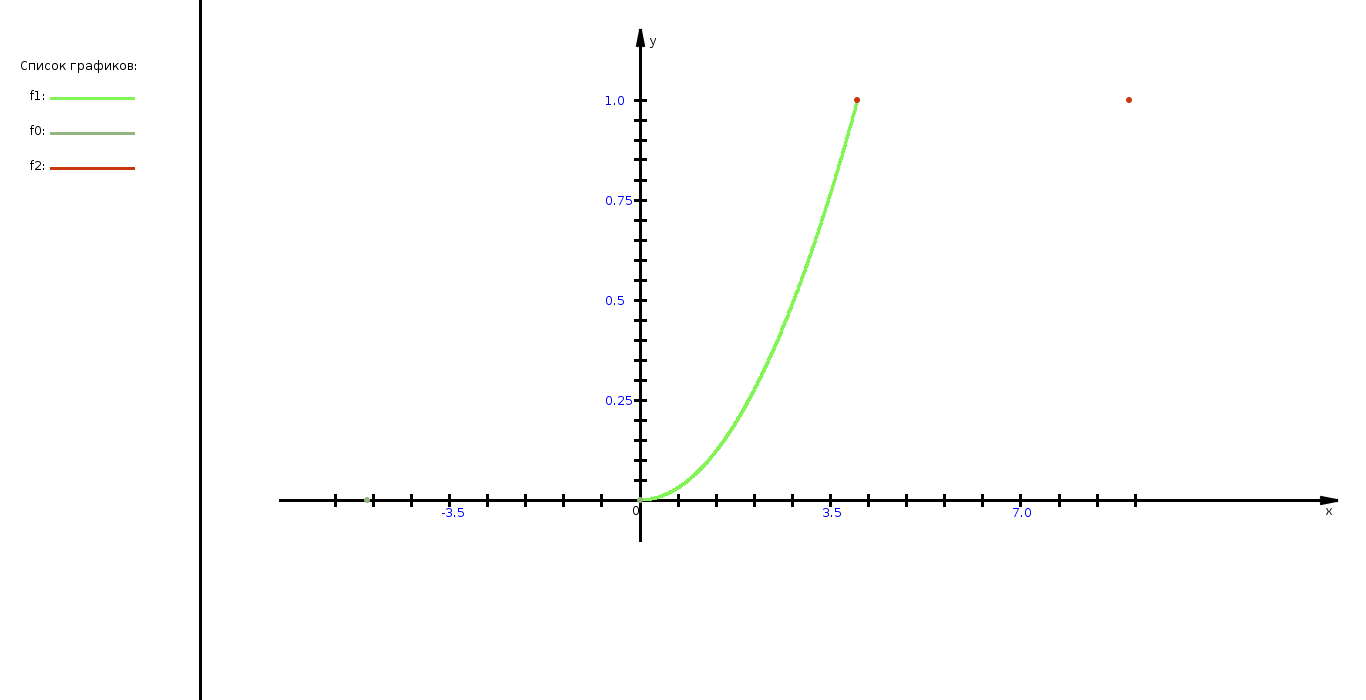
\includegraphics[width=300.57pt, height=192.835pt]{pictures/8_2}
\caption{Функция распределения непрерывной случайной величины из примера 2}
\label{8_2}
\end{figure}
%enddelete

\section{Функции дискретных случайных величин}
Дискретная случайная величина задается как  матрица,  имеющая две строки.  В первой строке записаны значения случайной величины,  во второй~--- соответствующие им вероятности.  То есть каждый элемент второй строки является числом на отрезке [$0$,  $1$], при  этом и сумма всех элементов второй  строки должна быть равна $1$.  
Например,  $DRQ=([1, 2, 3, 4, 5], [0.4, 0.1, 0.1, 0.2, 0.2]).$ 


Для дискретных случайных величин  определены следующие функции. 

\comm{mathExpectation}{(DRQ)} вычисляет математическое ожидание дискретной случайной величины $DRQ$. 

\comm{dispersion}{(DRQ)} вычисляет дисперсию дискретной случайной величины $DRQ$. 

\comm{meanSquareDeviation}{(DRQ)} вычисляет среднее квадратичное отклонение дискретной случайной величины $DRQ$. 

\comm{addQU}{(DRQ1, DRQ2)} складывает две дискретные случайные величины $DRQ1$ и $DRQ2$. 

\comm{multiplyQU}{(DRQ1, DRQ2)} умножает две дискретные случайные величины $DRQ1$ и $DRQ2$. 

\comm{covariance}{(DRQ1, DRQ2)} вычисляет коэффициент ковариации двух дискретных случайных величин $DRQ1$ и $DRQ2$. 

\comm{correlation}{(DRQ1, DRQ2)} вычисляет коэффициент корреляции двух дискретных случайных величин $DRQ1$ и $DRQ2$. 

\comm{plotPolygonDistribution}{(DRQ)} строит многоугольник распределения дискретной случайной величины $DRQ$. 

\comm{plotDistributionFunction}{(DRQ)} строит функцию распределения дискретной случайной величины $DRQ$. 

\comm{simplifyQU}{(DRQ)} упрощает дискретную случайную величину $DRQ$. 

\underline{Примеры.}

\vspace*{-2mm}
\begin{verbatim}
SPACE=R64[x]; 
DRQ=[[1, 2], [0.2, 0.8]];
g=\mathExpectation(DRQ); 
g1=\dispersion(DRQ); 
g2=\meanSquareDeviation(DRQ);  
\print(g, g1, g2);
\end{verbatim}
%begindelete 

\ex{$SPACE=R64[x];;$\\ 
\hspace*{4mm} $DRQ=\left(\begin{array}{cc}1& 2\\ 0.2& 0.8 \end{array}\right);$\\
\hspace*{4mm} $g=mathExpectation(DRQ);$\\ 
\hspace*{4mm} $g1=dispersion(DRQ);$\\ 
\hspace*{4mm} $g2=meanSquareDeviation(DRQ);$\\  
\hspace*{4mm} $print(g, g1, g2);$}
{$g = 1. 8; $\\
\hspace*{4mm} $g1 = 0.16; $\\
\hspace*{4mm} $g2 = 0.39;$} 

%enddelete
\begin{verbatim}
SPACE=R64[x]; 
DRQ=[[7, 5, 3, 5, 1], [0.2, 0.1, 0.3, 0.1, 0.3]];
g=\simplifyQU(DRQ); 
\print(g);
\end{verbatim}
%begindelete

\ex{$SPACE=R64[x];$\\ 
\hspace*{4mm} $DRQ=\left(\begin{array}{ccccc}   7& 5& 3& 5& 1\\ 0.2& 0.1& 0.3& 0.1& 0.3 \end{array}\right);$\\
\hspace*{4mm} $g=simplifyQU(DRQ);$\\ 
\hspace*{4mm} $print(g);$
}
{$g =\left(\begin{array}{cccc}1 &3 &5 &7 \\ 0.3 &0.3 &0.2 &0.2 \end{array}\right);$}

%enddelete
\begin{verbatim}
SPACE=R64[x]; 
DRQ1=[[0, 1], [0.33333, 0.66666]]; 
DRQ2=[[1, 2], [0.25, 0.75]];
g=\addQU(DRQ1, DRQ2); 
g1= \multiplyQU(DRQ1, DRQ2);  
\print(g, g1);
\end{verbatim}
%begindelete

\ex{$SPACE=R64[x];$\\ 
\hspace*{4mm} $DRQ1=\left(\begin{array}{cc} 0& 1\\ 0.33333& 0.66666  \end{array}\right); $\\
\hspace*{4mm} $DRQ2=\left(\begin{array}{cc} 1& 2\\ 0.25& 0.75 \end{array}\right);$\\
\hspace*{4mm} $g=addQU(DRQ1, DRQ2); $\\
\hspace*{4mm} $g1= multiplyQU(DRQ1, DRQ2); $\\ 
\hspace*{4mm} $print(g, g1);$}
{$g =\left(\begin{array}{ccc}1 & 2 & 3\\ 0.08 &0.41 &0.49 \end{array}\right) ; $\\
\hspace*{4mm} $g1 =\left(\begin{array}{ccc}0 & 1 & 2\\ 0.33 &0.16 &0.49 \end{array}\right);$} 

%enddelete
\begin{verbatim}
SPACE=R64[x];
DRQ=[[-7, -2, 0, 3, 5, 7, 9], 
  [0.3, 0.05, 0.2, 0.1, 0.1, 0.2, 0.05]];
\plotPolygonDistribution(DRQ);
\end{verbatim}
%begindelete


\ex{$SPACE=R64[x];$\\ 
\hspace*{4mm} $DRQ=\left(\begin{array}{ccccccc} -7& -2& 0& 3& 5& 7& 9\\ 0.3& 0.05& 0.2& 0.1& 0.1& 0.2& 0.05 \end{array}\right);$\\
\hspace*{4mm} $plotPolygonDistribution(DRQ);$}{рис. \ref{8_1}.}
                       
\begin{figure}[!ht]
 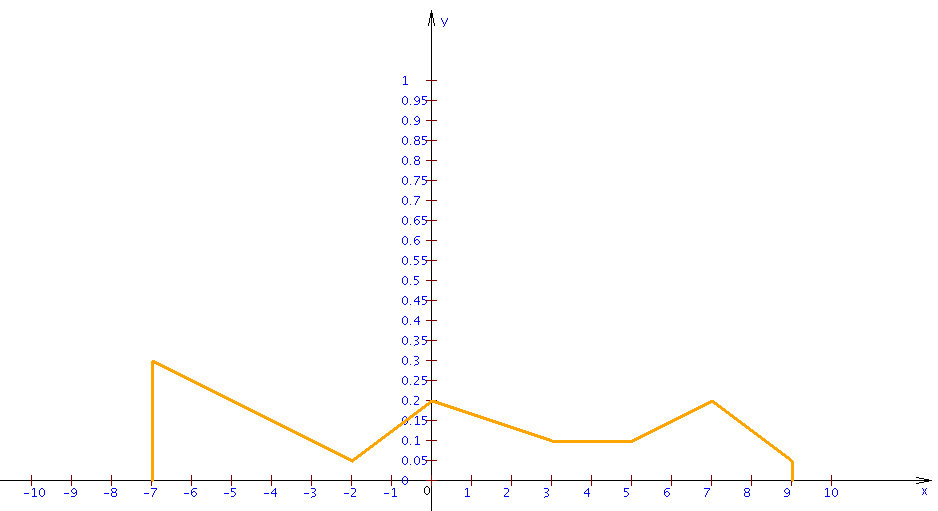
\includegraphics[width=300.57pt, height=192.835pt]{pictures/8_1}
\caption{Многоугольник распределения дискретной случайной величины из примера 4}
\label{8_1}
\end{figure}
%enddelete

\section{Функции для выборок}

Выборка задается как матрица из одной строки.  Например,  $[1, 7, 10, 15]$. 

\comm{sampleMean}{(S)} вычисляет выборочное среднее выборки $S$. 

\comm{sampleDispersion}{(S)} вычисляет выборочную дисперсию выборки $S$. 

\comm{covarianceCoefficient}{(S1, S2)} вычисляет коэффициент ковариации для 2 выборoк $S1$ и $S2$. 

\comm{correlationCoefficient}{(S1, S2)} вычисляет коэффициент корреляции для 2 выборoк $S1$ и $S2$. 

\underline{Пример. }

\vspace*{-2mm}
\begin{verbatim}
SPACE=R64[x];
S1=[0, 1]; 
S2=[1, 2];
g=\sampleMean(S1); 
g1=\sampleDispersion(S1); 
g2=\covarianceCoefficient(S1, S2); 
g3=\correlationCoefficient(S1, S2); 
\print(g, g1, g2, g3);
\end{verbatim} 
%begindelete

\ex{$SPACE=R64[x];$\\
\hspace*{4mm} $S1=[0, 1];$\\ 
\hspace*{4mm} $S2=[1, 2];$\\
\hspace*{4mm} $g=sampleMean(S1); $\\
\hspace*{4mm} $g1=sampleDispersion(S1); $\\
\hspace*{4mm} $g2=covarianceCoefficient(S1, S2); $\\
\hspace*{4mm} $g3=correlationCoefficient(S1, S2);$\\ 
\hspace*{4mm} $print(g, g1, g2, g3);$}
{$g = 0. 5; $\\
\hspace*{4mm} $g1 = 0.25; $\\
\hspace*{4mm} $g2 = 0.25; $\\
\hspace*{4mm} $g3 = 1.00$.} 
 
\section{Контрольные задания}
Заданы дискретные случайные величины $M$ и $K$\\
\begin{tabular}{c|c}
$M$&$K$\\
1 \hspace*{3mm} 1. 2 \hspace*{3mm} 1. 4 \hspace*{3mm} 1. 6 \hspace*{3mm} 1. 8\hspace*{3mm} & \hspace*{3mm} 0. 9 \hspace*{3mm} 1. 0 \hspace*{3mm} 1. 1 \hspace*{3mm} 1. 2 \hspace*{3mm} 1. 3\\
0. 1 \hspace*{1mm} 0. 1 \hspace*{3mm} 0. 3 \hspace*{3mm} 0. 4 \hspace*{3mm} 0. 1\hspace*{3mm} & \hspace*{3mm} 0. 2 \hspace*{3mm} 0. 3 \hspace*{3mm} 0. 2 \hspace*{3mm} 0. 2 \hspace*{5mm} 0. 1\\
\end{tabular}

В Mathpar найдите

\begin{itemize}
  \item математическое ожидание случайных величин $M$ и $K$, 
  \item дисперсию  случайных величин $M$ и $K$, 
  \item среднее квадратичное отклонение  случайных величин $M$ и $K$, 
  \item сумму,  произведение  случайных величин $M$ и $K$, 
  \item коэффициент ковариации  случайных величин $M$ и $K$, 
  \item коэффициент корреляции  случайных величин $M$ и $K$. 
  \item Постройте многоугольник распределения дискретной случайной величины $M$ и ее функции распределения. 
\end{itemize}
%enddelete

\chapter{Операторы управления.  Процедурное программирование}

\section{Процедуры и функции}
Система Mathpar позволяет создавать свои процедуры и функции.  Для этого используется команда \comm{procedure}{}.  После команды указывается имя процедуры и в фигурных скобках описывается сама процедура. 

\smallskip

\underline{Пример.}

\vspace*{-3mm}
 
\begin{verbatim}
\procedure myProc2() {
  d = 4;
  \print(d);
}
\procedure myProc(c,  d) {
  if (c < d) {
    \return d;
  } else {
    \return d+5;
  }
}
\myProc2();
a = 10;
c = \myProc(5 + a, a);
\print(a, c);
\end{verbatim}
%begindelete

 Результат выполнения: \\
$d = 4;\  
a = 10;\  
c = 15.$ 
%enddelete

\section{Операторы ветвления и циклов}

 Система Mathpar дает возможность использовать операторы ветвления и циклов. 

\comm{if }{()} \{ \} \comm{else}{} \{ \}~--- оператор ветвления; 

\comm{while }{()} \{ \}~--- оператор цикла с предусловием; 

\comm{for }{(\ ;\ ;\ )} \{ \}~--- оператор цикла с счетчиком.  

\smallskip

\underline{Примеры. }

\vspace*{-3mm}

\begin{verbatim}
a = 5; b = 1;
if (b < a) {
  b = b + a;
} else {
  \print(a, b);
}
if (b < a) {
  b = b + a;
} else {
  \print(a, b);
}
\end{verbatim}
%begindelete

Результат выполнения:\\
$a=5;\ b=6;$

%enddelete
\begin{verbatim}
a = 0;
b = 10;
while (a < b) {
  a = a + 5;
  \print(a);
}
\end{verbatim}
%begindelete

Результат выполнения:\\
$a = 5;$
$a = 10;$

%enddelete
\begin{verbatim}
for (i = 3; i \le 11; i = i + 5) { 
  \print(i);
}
\end{verbatim}

%begindelete
Результат выполнения:\\
$i = 3;$ 
$i = 8.$

\section{Контрольные задания}
В  Mathpar напишите программу:

\begin{itemize}
  \item для поиска наибольшего коэффициента матрицы, 
  \item для вывода всех чисел от 1 до 3000,  которые делятся на 252,  а при делении на 101 дают в остатке 3. 
\end{itemize}
%enddelete

\chapter{Calculations in idempotent algebras}


\section {Tropical algebras}
You can work in the following tropical algebras :

SEMIFIELDS\\
1) On the set of integers $ {\ mathbb Z} $ we define: \\
$ZMaxPlus$,  
$ZMinPlus$.\\
2) On the set of numbers ${\mathbb R}$ we define:\\
$RMaxPlus$, 
$RMinPlus$,  
$RMaxMult$,  
$RMinMult$.\\
3) On the set of numbers ${\mathbb R}64$ we define:\\
$R64MaxPlus$, 
$R64MinPlus$,  
$R64MaxMult$,  
$R64MinMult$.\\

SEMIRINGS\\
1) On the set of numbers ${\mathbb Z}$ we define:\\ 
$ZMaxMin$,
$ZMinMax$,
$ZMaxMult$,
$ZMinMult$.\\
2) On the set of numbers ${\mathbb R}$ we define:\\
$RMaxMin$, 
$RMinMax$.\\
3) On the set of numbers ${\mathbb R}64$ we define:\\
$R64MaxMin$, 
$R64MinMax$.

 

Examples of tropical algebras: 

SPACE = ZMaxPlus [x,  y,  z]; 

SPACE = R64MinMult [u,  v];  

SPACE = RMaxMin [u,  v]. 

 An example of a simple problem in a semiring
 $ZMaxMult$.
%begindelete
\smallskip

\underline{Example 1. }

%\vspace*{-2mm}
%enddelete
\begin{verbatim}
SPACE = ZMaxMult[x, y];
a = 2; b = 9; c = a + b; d = a*b; \print(c, d)
\end{verbatim}
%begindelete

Returns:\\
$c = 9; $\\
$d = 18.$
%enddelete

In the remaining sections of this chapter we have given some examples of problems that are solved in the tropical algebra, which are semi-fields.
%begindelete
\section{Solving systems of linear algebraic equations}
The command $\backslash solveLAETropic(A, b)$ enables us to find a particular solution of the system 
$Ax = b$.
%begindelete
\smallskip

\underline{Example 2. }

%\vspace*{-2mm}
%enddelete
\begin{verbatim}
SPACE = R64MaxPlus[x, y];
A = [
  [1.00, 1.00, 0.00],
  [2.00, 0.00, 3.00],
  [3.00, 4.00, 2.00]
];
b = [8.00, 7.00, 11.00];
X = \solveLAETropic(A, b); 
\print(X);
\end{verbatim}
%begindelete

Returns:\\
$X = \left(\begin{array}{c}
5.00\\
7.00\\
4.00\\
\end{array}\right)
$ 
%enddelete
 
\section{Solving systems of linear algebraic inequalities}
The command $\backslash solveLAITropic(A,b)$ enables us to find a particular solution of the system of inequalities 
%begindelete
\smallskip

\underline{Example 3. }

\vspace*{-3mm}
%enddelete
\begin{verbatim}
SPACE = R64MaxPlus[x, y];
A = [
  [1.00, 1.00, 0.00],
  [2.00, 0.00, 3.00],
  [3.00, 4.00, 2.00]
];
b = [10.00, 7.00, 11.00]; 
X = \solveLAITropic(A, b); 
\print(X);
\end{verbatim}
%begindelete

Returns:\\
$X=[(-\infty,5.00],(-\infty,7.00],(-\infty,4.00]]$ 
%enddelete

%begindelete
\smallskip

\underline{Example 4. }

\vspace*{-3mm}
%enddelete
\begin{verbatim}
SPACE = ZMinPlus[x, y];
A = [
  [1, 1, 0],
  [2, 0, 3],
  [3, 4, 2]
];
b = [10, 7, 11];
X = \solveLAITropic(A, b); 
\print(X);
\end{verbatim}
%begindelete

Returns:\\
$X=[[9,\infty),[9,\infty),[10,\infty)]$ 
%enddelete

\section{The solution of the Bellman equation}
\subsection {The homogeneous  Bellman equation}
The command $\backslash BellmanEquation(A)$ enables us to find a solution of the homogeneous  Bellman equation
  $Ax = x$.
%begindelete
\smallskip

\underline{Example 5.}

\vspace*{-3mm}
%enddelete
\begin{verbatim}
SPACE = R64MaxPlus[x, y];
A = [
  [0.00, -2.00, -\infty, -\infty],
  [-\infty, 0.00, 3.00, -1.00],
  [-1.00, -\infty, 0.00, -4.00],
  [2.00, -\infty, -\infty, 0.00]
]; 
X = \BellmanEquation(A); 
\print(X);
\end{verbatim}
%begindelete

Returns:\\
$$
X=\left(\begin{array}{cccc}
0.00 & -2.00 & 1.00 & -3.00\\
2.00 & 0.00 & 3.00 & -1.00\\
-1.00 & -3.00 & 0.00 & -4.00\\
2.00 & 0.00 & 3.00 & 0.00
\end{array}\right) \left(\begin{array}{c}
v_{1}\\
v_{2}\\
v_{3}\\
v_{4}
\end{array}\right), \forall v_{1}, v_{2}, v_{3}, v_{4}.$$
%enddelete
\subsection {The inhomogeneous  Bellman equation}
The command $\backslash BellmanEquation(A,b)$ enables us to find a solution of the inhomogeneous  Bellman equation $Ax\oplus b=x$.
%begindelete
\smallskip

\underline{Example 6. }

\vspace*{-3mm}
%enddelete
\begin{verbatim}
SPACE = R64MaxPlus[x, y];
A = [
  [0.00, -2.00, -\infty, -\infty],
  [-\infty, 0.00, 3.00, -1.00],
  [-1.00, -\infty, 0.00, -4.00],
  [2.00, -\infty, -\infty, 0.00]
];
b = [[1], [-\infty], [-\infty], [-\infty]]; 
X = \BellmanEquation(A, b); 
\print(X);
\end{verbatim}
%begindelete

Returns:\\
$$X=
 \left(\begin{array}{cccc}
0.00 & -2.00 & 1.00 & -3.00\\
2.00 & 0.00 & 3.00 & -1.00\\
-1.00 & -3.00 & 0.00 & -4.00\\
2.00 & 0.00 & 3.00 & 0.00
\end{array}\right)
\left(\begin{array}{c}
v_{1}\\
v_{2}\\
v_{3}\\
v_{4}
\end{array}\right)
\oplus\left(\begin{array}{c}
1.00\\
3.00\\
0.00\\
3.00
\end{array}\right),$$\\ $$\forall v_{1}, v_{2}, v_{3}, v_{4}.$$
%enddelete
\section{The solution Bellman inequality}
\subsection{The homogeneous Bellman inequality}
 
The command $\backslash BellmanInequality(A)$ enables us to find a solution of the homogeneous Bellman inequality $Ax\leq x$.

\subsection{The inhomogeneous Bellman inequality}
The command $\backslash BellmanInequality(A, b)$ enables us to find a solution of the inhomogeneous Bellman inequality $Ax\oplus b\leq x$.

\section{Finding the shortest path between the vertices of the graph}
\subsection {Calculation of the table of shortest distances for all vertices of the graph}
Let $A=(x_{ij})$ be matrix of distances between adjacent vertices. We put $x_{ii}$=0 $\forall i$ and we put $x_{ij}=\infty$, if there is no edge connecting vertices i and j.
The command $\backslash searchLeastDistances(A)$ allows you to find the smallest distance between all the nodes of the graph.
This results in a matrix of shortest paths between all vertices.
 
%begindelete
\smallskip

\underline{Example 7. }

\vspace*{-3mm}
%enddelete
\begin{verbatim}
SPACE = R64MinPlus[x, y];
A = [
  [0.00, 7.00, 9.00, \infty, \infty, 14.00],
  [7.00, 0.00, 10.00, 15.00, \infty, \infty],
  [9.00, 10.00, 0.00, 11.00, \infty, 2.00],
  [\infty, 15.00, 11.00, 0.00, 6.00, \infty],
  [\infty, \infty, \infty, 6.00, 0.00, 9.00],
  [14.00, \infty, 2.00, \infty, 9.00, 0.00]
];
B = \searchLeastDistances(A);
\print(B);
\end{verbatim}
%begindelete

Returns:\\
$$B= \left(\begin{array}{cccccc}
0.00 & 7.00 & 9.00 & 20.00 & 20.00 & 11.00\\
7.00 & 0.00 & 10.00 & 15.00 & 21.00 & 12.00\\
9.00 & 10.00 & 0.00 & 11.00 & 11.00 & 2.00\\
20.00 & 15.00 & 11.00 & 0.00 & 6.00 & 13.00\\
20.00 & 21.00 & 11.00 & 6.00 & 0.00 & 9.00\\
11.00 & 12.00 & 2.00 & 13.00 & 9.00 & 0.00
\end{array}\right) $$
%enddelete
\subsection {Calculation of the shortest distances between two vertices of the graph}
Let $A=(x_{ij})$ be matrix of distances between adjacent vertices. We put $x_{ii}$=0 $\forall i$ and we put $x_{ij}=\infty$, if there is no edge connecting vertices $i$ and $j$.

The command $\backslash findTheShortestPath(A, i, j)$ allows you to find the shortest path between nodes $i$ and $j$.
 %begindelete
\smallskip

\underline{Example 8. }

\vspace*{-3mm}
%enddelete
\begin{verbatim}
SPACE = R64MinPlus[x, y];
A = [
  [0.00, 7.00, 9.00, \infty, \infty, 14.00],
  [7.00, 0.00, 10.00, 15.00, \infty, \infty],
  [9.00, 10.00, 0.00, 11.00, \infty, 2.00],
  [\infty, 15.00, 11.00, 0.00, 6.00, \infty],
  [\infty, \infty, \infty, 6.00, 0.00, 9.00],
  [14.00, \infty, 2.00, \infty, 9.00, 0.00]
];
X = \findTheShortestPath(A, 0, 4);
\print(X);
\end{verbatim}
%begindelete

Returns:\\
$X=[[0, 2, 5, 4]]$
%enddelete
 

\chapter{Вычисления на суперкомпьютере}

Для решения вычислительных задач, требующих большого времени вычислений или больших объемов памяти,  разработаны специальные функции,  которые предоставляют пользователю ресурсы 
суперкомпьютера.  При использовании этих функций вычисления производятся не на одном процессоре,  а на выделенном множестве ядер суперкомпьютера,  количество которых заказывает пользователь. 
Имеются следующие функции,  которые используют суперкомпьютер (парфункции). 

1) \comm{matMultPar1x8}{}~--- вычисление произведения двух матриц;

2) \comm{adjointDetPar}{}~--- вычисление присоединенной матрицы;

3) \comm{charPolPar}{}~--- вычисление характеристического полинома матрицы;

4) \comm{polMultPar}{}~--- вычисление произведения двух полиномов;

5) \comm{BellmanEquationPar}{A}~--- решение однородного уравнения Беллмана $Ax=x$;

6) \comm{BellmanEquationPar}{A,b}~--- решение однородного уравнения Беллмана $Ax+b=x$;

7) \comm{BellmanInequalityPar}{A}~--- решение однородного неравенства Беллмана $Ax\leq x$;

8) \comm{BellmanInequalityPar}{A,b}~--- решение однородного неравенства Беллмана $Ax+b\leq x$; 

 
До применения любой из этих функций пользователь должен указать параметры,  определяющие параллельное окружение: 

$TOTALNODES$~--- общее количество узлов кластера, которые выделяются для вычислений,  

$PROCPERNODE$~--- количество MPI-процессов, запускаемых на одном узле,   

$CLUSTERTIME$~--- максимальное время (в минутах) выполнения программы,  после истечения которого программа принудительно завершится,

$MAXCLUSTERMEMORY$~--- объем памяти, выделяемый для JVM для одного MPI-процесса (опция -Xmx).

Для задания количества ядер на одном узле пользователь должен знать, какой кластер используется и сколько доступно ему ядер на узле.  По умолчанию параметры $TOTALNODES$ и  $PROCPERNODE$ устанавливаются так,  чтобы использовалась половина всех узлов кластера и на каждом узле было запущено по одному процессу,  а $CLUSTERTIME$ двум минутам. Если на одном узле запускается $K$ процессов, то каждому из них будет выделено $MAXCLUSTERMEMORY/K$ мегабайт памяти. 


\section{Параллельные полиномиальные вычисления}
  Для параллельного вычисления произведения полиномов надо использовать команду 
  \comm{polMultPar}{(p1, p2)},  где $p1$,  $p2$~--- входные полиномы.  

\underline{Пример. }
\begin{verbatim}
TOTALNODES = 2;
PROCPERNODE = 1;
A=x^2+3y;
B=x^2+3y+3z;
\polMultPar(A, B);
\end{verbatim}

      
\section{Параллельные матричные вычисления}
  Для параллельного вычисления произведения матриц $m1$ и $m2$ необходимо использовать команду 
  \underline{Пример. }
\begin{verbatim}
TOTALNODES = 2;
PROCPERNODE = 1;
A=[[0,1],[2,3]];
B=[[0,1],[2,3]];
\matMultPar1x8(A, B);
\end{verbatim}
 
  Для параллельного вычисления присоединенной матрицы для матрицы $m$ можно использовать команду 
   \underline{Пример. }
\begin{verbatim}
TOTALNODES = 2;
PROCPERNODE = 1;
SPACE = Z[x];
A=[[0,1],[2,3]];   
\adjointDetPar(A);
\end{verbatim}
 
 
\section{Запуск собственных параллельных программ}
  Mathpar позволяет загружать и исполнять собственные параллельные программы.
  Пакет с программой должен распологаться в корневой директории проекта mathpar.
  Для того, чтобы ваша программа смогла взаимодействовать с системой управления заданиями,
  необходимо в ваш main-метод добавить строку инициализации QueryResult queryRes=Tools.getDataFromClusterRootNode(args)
 (сразу после MPI.Init) и  строку завершения Tools.sendFinishMessage(args) (перед MPI.Finalize),
  этот код будет одинаков для всех ваших программ).   Также вы можете передать вашей программе 
  любые аргументы из web-интерфейса Mathpartner.  Внутри программы их можно получить, вызвав 
метод queryRes.getData(). Ниже приведен пример параллельной программы, 
которая просто выводит в стандартный поток вывода  переданные ей аргументы .

\begin{verbatim}
        MPI.Init(args);
        QueryResult queryRes=Tools.getDataFromClusterRootNode(args);
        int myRank=MPI.COMM_WORLD.getRank();
        if (myRank == 0) {
            Object []ar=queryRes.getData();
            System.out.println("test...");           
            for (int i=0; i<ar.length; i++){
                System.out.println(((Element)ar[i]).intValue());
            }            
        }
        Tools.sendFinishMessage(args);
        MPI.Finalize();
\end{verbatim}


  Далее программу нужно скомпилировать, и папку с программой запаковать в zip-архив.
  Затем нужно загрузить полученный архив на сервер, воспользовавшись вкладкой "файлы" и нажав кнопку "загрузить файл".
  Далее вся работа будет выполняться с помощью функций mathpar. 

Оперативная память делится между всеми ядрами процессора поровну. Для примера, если на узле кластера имеется 8GB памяти,
то если вы запросили 4 ядра на одном процессоре, каждому будет выделено 2GB, а если одно ядро - то оно получит все 8GB.

Команда для загрузки вашего zip-архива, в котором скомпилированные java-классы,
выглядит следующим образом:

 \comm{uploadToCluster}{(FileName)}, где FileName - имя zip-архива.

Чтобы просмотреть список всех ваших загруженных на кластер файлов, используется команда

 \comm{showFileList}{()}.


Для запуска вашей программы используется команда

\comm{runUploadedClass}{(archieveName, classPath, param0, param1,...)},
где archieveName - имя загруженного zip-архива с программой, classPath - путь до класса, содержащего main-метод (с указанием пакетов),
paramX - произвольные параметры, указанные через запятую, которые будут переданы в вашу программу.

Чтобы следить за работой запущенной программы, используется команда 

\comm{getStatus}{(taskID)}

Также имеется возможность получить список всех задач текущего пользователя с описанием их состояний:

\comm{showTaskList}{()}

Для того, чтобы получить содержимое файлов с потоком стандартного вывода/ошибок, используются команды

\comm{getOut}{(taskID)}

\comm{getErr}{(taskID)}

Файлы задачи (файлы, содержащие поток вывода/ошибок) хранятся на кластере двое суток,
zip-архивы, содержащие скомпилированные java-классы, хранятся 30 дней.


\chapter{Список операторов}

{\bf Правило образования наименований математических объектов}
\bigskip

Заглавные и строчные буквы всюду различаются. Пользователь может давать любые имена для математических объектов. Однако эти имена не должны совпадать с операторами и константами, которые определены в системе. Кроме того, имена объектов, умножение которых  не коммутативно,  например,  векторов и матриц,  должны начинаться с заглавных латинских букв, а все остальные имена объектов должны начинаться со строчных букв. Это дает возможность сразу после ввода автоматически получать упрощенное выражение.
\bigskip

Приведем список основных операторов системы Mathpar.   

\comm{clean}{}~---  удаление всех введенных имен объектов.  Если в операторе перечислены имена объектов,  то удаляются только объекты с этими именами. 
\bigskip

{\bf Инфиксные арифметические операторы}

{\bf +}~---   сложение;

{\bf -}~---  вычитание;

{\bf /}~---  деление;

{\bf *}~---  умножение (можно использовать пробел вместо знака умножения);

\comm{times}{}~--- некоммутативное умножение. 
\bigskip


\bigskip

{\bf Постфиксные арифметические операторы}


{\bf !}~---  факториал;

{ ${x} \widehat{\ }{\{ \}}$}~---  возведение в степень;
\bigskip

{\bf Инфиксные операторы сравнения.}


$\mathbf{\backslash le}$~---  меньше или равно;

{\bf >}~---  больше;

 $\mathbf{\backslash ge}$~--- больше или равно;

{\bf ==}~---   равно;

$\mathbf{\backslash ne}$~--- неравно. 
\bigskip

{\bf Инфиксные логические операторы}


 $\mathbf{ \backslash lor}$ ~--- дизъюнкция;

 $\mathbf{ \backslash  \&}$~--- конъюнкция;

 $\mathbf{ \backslash neg}$ ~--- отрицание. 


{\bf Основные префиксные операторы}

 \comm{d}{}~--- символ дифференцирования при записи дифференциального уравнения;

 \comm{D}{}~--- производная функции: \comm{D}{(f)} и \comm{D}{(f, x)}~--- первая производная по $x$; $\mathbf D (f, y\widehat{\ }{}3)$~--- третья производная по $y$ и т. д.;

 \comm{expand}{}~--- преобразование выражения в сумму с раскрытием всех скобок в выражении;

 \comm{fullExpand}{}~--- преобразование в сумму выражения, которое содержит логарифмические, показательные и тригонометрические функции;

 \comm{extendedGCD}{}~--- расширенный алгоритм вычисления наибольшего общего делителя (НОД) полиномов.  В результате получается вектор,  содержащий НОД и дополнительные множители аргументов;

 \comm{GCD}{}~--- вычисление НОД полиномов;

 \comm{factor}{}~--- представление выражения в виде произведения;

 \comm{fullFactor}{}~--- представление выражения,  содержащего логарифмические и показательные функции,  в виде произведения;

 \comm{initCond}{}~--- задание начальных условий для системы линейных дифференциальных уравнений;

 \comm{LCM}{}~--- вычисление наименьшего общего кратного (НОК) полиномов;

 \comm{lim}{}~--- предел выражения;

 \comm{print}{}~--- печать выражений. Аргументами выступают имена выражений, разделенные запятыми. Каждое выражение будет печататься на новой строке;

 \comm{printS}{}~--- печать выражений в одну строчку, для перехода на следующую строчку нужно использовать <<$\backslash$n>>;

 \comm{plot}{}~--- построение графика функции, которая задана явно;
 
  \comm{plot3D}{}~--- построение графика функции двух переменных, которая задана явно;

 \comm{paramPlot}{}~--- построение графика функции, которая задана  параметрически; 

\comm{tablePlot}{}~--- построение графика функции,  заданной таблицей аргументов и значений;

 \comm{prod}{}~--- произведение (символ $\prod$);

 \comm{randomPolynom}{}~--- генерация случайного полинома;

 \comm{randomMatrix}{}~--- генерация случайной матрицы;

 \comm{randomNumber}{}~--- генерация случайного числа;

 \comm{sequence}{}~--- задание последовательности;

 \comm{showPlots}{}~--- построение в одной системе координат графиков функций, которые должны быть определены раньше;

 \comm{solveLDE}{}~--- решение систем линейных дифференциальных уравнений;

 \comm{systLAE}{}~--- задание систем линейных алгебраических уравнений;

 \comm{systLDE}{}~--- задание систем линейных дифференциальных уравнений;

 \comm{sum}{}~---  сумма (символ $\sum$);

 \comm{time}{}~--- определение процессорного времени в миллисекундах;

 \comm{value}{}~--- вычисление значение выражения при подстановке заданных выражений или чисел вместо переменных кольца.

 \bigskip
 
 {\bf Операторы процедуры,  ветвления и цикла}

 \comm{procedure}{}~--- оператор объявления процедуры; 
 
\comm{if }{(\ ) \{\  \}} \comm{else }{\{ \ \}}~--- оператор ветвления; 

\comm{while }{( \ ) \{ \ \}}~--- оператор цикла с предусловием; 

\comm{for }{(\ ; \ ; \ ) \{ \ \}}~--- оператор цикла с счетчиком.  
\bigskip

{\bf Матрицы, их элементы и матричные операторы}

[\ , \  ] ~--- задание вектора (строки);

[[\ ,\  ], [\ ,\  ]]~--- задание матрицы;


A\_\{i,j\}~--- (i,j)-элемент матрицы A;  

A\_\{i,?\}~---  строка i матрицы A; 

A\_\{?,j\}~--- столбец j  матрицы A; 

$\backslash$O\_\{n,m\}~--- нулевая матрица размера $n \times m$ ; 

$\backslash$I\_\{n,m\}~---  $n \times m$ матрица  с единицами на главной диагонали; 

+, -, *~--- сложение,  вычитание,  умножение; 

\comm{charPolynom}{}~---  характеристический полином;
 
\comm{kernel}{}~--- ядро оператора (нуль-пространство);

\comm{transpose}{} или  $\mathbf{A \widehat{\ } \{T\}}$~--- транспонированная матрица;
 
\comm{conjugate}{} или  $\mathbf{A\widehat{\ }\{\backslash ast\}}$~--- сопряженная матрица;

\comm{toEchelonForm}{}~---   эшелонная (ступенчатая) форма; 

\comm{det}{}~---   определитель;
 
\comm{inverse}{}  или  $\mathbf{A\widehat{\ }\{-1\}}$~--- обратная матрица;

\comm{adjoint}{}  или  $\mathbf{A\widehat{\ }\{\backslash star\}}$~--- присоединенная матрица;
 
\comm{genInverse}{} или $\mathbf{A\widehat{\ }\{+\}}$~--- обобщенная обратная матрица Мурра-Пенроуза;
 
\comm{closure}{}  или $\mathbf{A\widehat{\ }\{\backslash times\}}$~--- замыкание,  т.е. сумма $I+A+A^2+A^3+\ldots$. Для классических алгебр это эквивалентно $(I-A)^{-1}$; 

\comm{LDU}{} --- LDU-представление матрицы. Результат~--- вектор из трёх матриц $[L,D,U]$. Здесь $L$~--- нижняя треугольная матрица, $U$~--- верхняя треугольная матрица, 
$D$~--- матрица перестановок, умноженная на обратную к диагональной матрицу.

\comm{BruhatDecomposition}{} --- разложение Брюа матрицы. Результат~--- вектор из трёх матриц $[V,D,U]$. Здесь  $V$ и $U$~--- верхние треугольные матрицы, 
$D$~--- матрица перестановок, умноженная на матрицу, которая является обратной к диагональной матрице.


\chapter{ Examples of solutions of physical problems }

\section{Transferring of the  heat}
 
\begin{verbatim}
"EXERCISE 1"
"A piece of ice which has mass"
M = 10 kg;
"was put in a vessel. The ice has temperature ($\degreeC$)"
T = -10  \degreeC ;
"Find the mass of water in a vessel after transferring the"
q = 20000 kJ
"amount of heat. Specific heat of water heating is equal"
c_v = 4.2 kJ/(kg \degreeC);
"Specific heat of ice heating is equal"
c_i = 2.1 kJ/(kg \degreeC);
"The heat of fusion of ice is equal"
r = 330 kJ/kg;
"Specific heat of vaporization of water is equal"
\lambda = 2300 kJ/kg;
END
\end{verbatim}

\vspace*{-3mm}

\begin{verbatim}
"SOLUTION OF EX. 1."
SPACE = R64[x];
"Unknown mass of water is denoted by x.
The amount of heat: to heat the ice to 0 degrees:"
q_1 = M c_i (0 - T);
"to melt the ice:"
q_2 = M r;
"to heat water to 100 degrees:"
q_3 = M c_v (100 \degreeC);
"to evaporation of water"
q_4 = (M - x) \lambda;
"we denote by x unknown value."
"By assumption, we obtain the equation"
mass = \solve(q = q_1 + q_2 + q_3 + q_4); 
\print(mass);
\end{verbatim}

\vspace*{-3mm}

\section{Kinematics} 

\begin{verbatim}
"EXERCISE 2" 
"Kinematic equation of motion of a point in a straight line (axis x) 
has the form $x = c_1 + c_2 * t + c_3 t^3$."
"Define: (1) coordinate of a point, (2) the instantaneous velocity,
(3) the instantaneous acceleration "
END
\end{verbatim}

\vspace*{-3mm}

\begin{verbatim}
"SOLUTION OF EX.2."
"Let us set the space with variables $t, c_1, c_2, c_3$:"
SPACE = R64[t, c_1, c_2, c_3];
"The equation of motion is"
x = c_1 + c_2 t + c_3 t^3;
"We can find the instant speed"
v = \D_t(x);
"We can find the instant acceleration"
a = \D_t(v);
\print(x, v, a);
\end{verbatim}

\vspace*{-3mm}

\begin{verbatim}
"EXERCISE 2A"
"Solve the previous problem at a moment of time"
t_0 = 2 "seconds"
"with the following numerical values:
$c_1=4; c_2=2; c_3=-0.5$."
END
\end{verbatim}

\vspace*{-3mm}

\begin{verbatim}
"SOLUTION OF EX.2A."
arg = [t_0, 4, 2, -0.5];
x_0 = \value (x, arg);  
v_0 = \value (v, arg);
a_0 = \value (a, arg);
\print(x_0, v_0, a_0);
\end{verbatim}

\vspace*{-3mm}

\section{Molecular Physics} 

\begin{verbatim}
"EXERCISE 3"
"In the middle of the horizontal tube was placed a drop of mercury in length h." 
"The air was pumped out of the tube and the ends 
of the tube was sealed. Tube length is equal l." 
"When the tube was placed vertically, a drop of mercury moved down by $l_d$."
"The acceleration of gravity is equal g."
"The density of mercury is equal $\rho$."
"What was the initial pressure in the  tube?"
END
\end{verbatim}

\vspace*{-3mm}

\begin{verbatim}
"SOLUTION OF EX. 3."
"Let the initial pressure $p_0$ be unknown:"
SPACE = R64[p_0];
"The pressure at the bottom of the tube increased, as added
pressure mercury drops, so new pressure is equal:"
p_1 = p_0 + \rho g h;
"Let S be the cross-sections of the tube. Then
the initial volume of air in the bottom of the tube is equal:"
v_0 = (l/2 - h/2) S;
"After turning the tube  volume of air in the bottom of the tube is equal:"
v_1 = (l/2 - h/2 - l_d) S;
"According  to Boyle–Mariotte law we have the equation:"
initialPressure = \solve(p_0 v_0 = p_1 v_1);
\print(initialPressure);
\end{verbatim}

\vspace*{-3mm}

\begin{verbatim}
"EXERCISE 3A"
"Solve the previous problem with the following numerical values: "
h = 0.20 m;
l = 1 m;
l_d = 0.10 m;
"The acceleration of gravity is equal"
g = 9.8 m/s^2;
\rho = 13600 kg/m^3;
END
\end{verbatim}

\vspace*{-3mm}

\begin{verbatim}
"SOLUTION OF EX. 3A."
p_1 = p_0 + \rho g h;
v_0 = (l/2 - h/2) S; 
v_1 = (l/2 - h/2 - l_d) S;
initialPressure = \solve(p_0 v_0 = p_1 v_1);
\print(initialPressure);
\end{verbatim}

%
\chapter{ דוגמאות לפתרונות של בעיות פיזיות  }

\section{הטרנספורמציה של החום}
 
\begin{verbatim}
"תרגיל 1"
"חתיכת הקרח שבו יש מסה"
M = 10 kg;
"הוכנסה לכלי. הטמפרטורה של הקרח"
T = -10  \degreeC ;
"מצא את המסה של מים בכלי לאחר הטרנספורמציה. כמות של חום"
q = 20000 kJ
"חום ספציפי לחימום מים היא שווה ל"
c_v = 4.2 kJ/(kg \degreeC);
"חום ספציפי לחימום קרח שווה ל"
c_i = 2.1 kJ/(kg \degreeC);
"חום ההיתוך של קרח הוא שווה ל"
r = 330 kJ/kg;
"חום האידוי של מים הוא שווה"
\lambda = 2300 kJ/kg;
END
\end{verbatim}

\vspace*{-3mm}

\begin{verbatim}
"פתרון תרגיל 1"
SPACE = R64[x];
"  .x מסה לא ידועה של מים מסומן ב  
כמות החום : כדי לחמם את הקרח ל 0 מעלות"
q_1 = M * c_i * (0 - T);
" כדי להמס את הקרח "
q_2 = M * r;
" כדי לחמם את המים ל 100 מעלות "
q_3 = M * c_v * (100 \degreeC);
" לאידוי של המים "
q_4 = (M - x) \lambda;
"  ערך ידוע x נסמן על ידי "
" על ידי הנחה, נקבל את המשוואה"
mass = \solve(q = q_1 + q_2 + q_3 + q_4); 
\print(mass);
\end{verbatim}

\vspace*{-3mm}

\section{קינמטיקה} 

\begin{verbatim}
"תרגיל 2"
" : יש את הצורה (x משוואה קינמטית של תנועה, של נקודה בקו ישר (על גבי ציר ה  
 $x = c_1 + c_2 * t + c_3 * t^3$ "
"הגדר: (1) קואורדינטות של נקודה, (2) המהירות הרגעית 
  את התאוצה הרגעית  "
END
\end{verbatim}

\vspace*{-3mm}

\begin{verbatim}
"פתרון תרגיל 2"
" $t, c_1, c_2, c_3$: נגדיר את הרווחים עם המשתנים"
SPACE = R64[t, c_1, c_2, c_3];
"משוואת התנועה היא"
x = c_1 + c_2 t + c_3 t^3;
"אנחנו יכולים למצוא את המהירות הרגעית"
v = \D_t(x);
"אנחנו יכולים למצוא את התאוצה הרגעית"
a = \D_t(v);
\print(x, v, a);
\end{verbatim}

\vspace*{-3mm}

\begin{verbatim}
"תרגיל 2 ב"
"לפתור את הבעיה הקודמת ברגע של זמן"
t_0 = 2 "שניות"
"עם הערכים המספרים הבאים"
"$c_1=4; c_2=2; c_3=-0.5$."
END
\end{verbatim}

\vspace*{-3mm}

\begin{verbatim}
"פתרון תרגיל 2 ב"
arg = [t_0, 4, 2, -0.5];
x_0 = \value (x, arg);  
v_0 = \value (v, arg);
a_0 = \value (a, arg);
\print(x_0, v_0, a_0);
\end{verbatim}

\vspace*{-3mm}

\section{פיסיקה מולקולרית} 

\begin{verbatim}
"תרגיל 3"
" H באמצע צינור אופקי, הונחה טיפה של כספית באורך" 
" L האוויר נשאב החוצה מהצינור והקצוות של הצינור נאטמו. אורך צינור שווה ל" 
" $L_d$ כאשר הצינור הונח במאונך, טיפה של כספית זזה למטה במרחק של"
"g  תאוצת כוח המשיכה שווה ל"
"$\rho$  הצפיפות הכספית שווה ל"
"?מה הלחץ הראשוני בצינור "
END
\end{verbatim}

\vspace*{-3mm}

\begin{verbatim}
"פתרון תרגיל 3"
" לא ידוע $p_0$ נניח והלחץ הראשוני בצינור"
SPACE = R64[p_0];
"הלחץ בחלקו התחתון של הצינור גדל, ככל שהוסיפה "
"הכספית לרדת, ולכן הלחץ חדש שווה ל"
p_1 = p_0 + \rho * g * H;
".היא נקודת ההצטלבות של הצינור S נניח ש"
":אז הנפח הראשוני של אוויר בחלק התחתון של הצינור שווה "
v_0 = (L/2 - H/2) * S;
"לאחר סיבוב הצינור, נפח האוויר בחלק התחתון של הצינור הוא שווה ל"
v_1 = (L/2 - H/2 - L_d) * S;
" מתקבלת המשוואה Boyle–Mariotte על פי חוק"
initialPressure = \solve(p_0 * v_0 = p_1 * v_1);
\print(initialPressure);
\end{verbatim}

\vspace*{-3mm}

\begin{verbatim}
"תרגיל 3 ב"
"לפתור את הבעיה הקודמת עם הערכים המספרים הבאים"
H = 0.20 m;
L = 1 m;
L_d = 0.10 m;
"תאוצת הכובד שווה ל"
g = 9.8 m/s^2;
\rho = 13600 kg/m^3;
END
\end{verbatim}

\vspace*{-3mm}

\begin{verbatim}
"פתרון תרגיל 3 ב"
p_1 = p_0 + \rho g H;
v_0 = (L/2 - H/2) S; 
v_1 = (L/2 - H/2 - L_d) S;
initialPressure = \solve(p_0 v_0 = p_1 v_1);
\print(initialPressure);
\end{verbatim}

%
\chapter{ דוגמאות לפתרונות של בעיות מתמטיות }

\section{סידרה  חשבונית}
 
\begin{verbatim}
"TASK-Z:  תרגיל  סידרה  חשבונית.
$( n > 2) $   איברים  n   נחונה  סידרה  חשבונית  שיש  בה
 $a_1, a_2, a_3, … , a_{n-1}, a_n$
$d$  :  הפרש  הסידרה  הוא
מהסידרה  הנתונה  בנו  סידרה  חדשה
$  a_{2}^2 – a_{1}^2,  a_{3}^2 – a_{2}^2, …,  a_{n}^2 – a_{n-1}^2$
$2d^2$   הוכח כי  סידרה  חדשה  היא  סידרה  חשבונית  שהפרשה  הוא
$a_{2}^2 – a_{1}^2 = 64$  :    נחון   
$d$ , $n$   הבע  את  האיבר  האחרון  בסידרה  החדשה  באמצעות 
$ a_{n}^2 – a_{n-1}^2 = 192  ,   d > 1 $  :    נחון גם
$n$   מצא  את  תחום  הערכים  של "
 END
\end{verbatim}

\vspace*{-3mm}  

\begin{verbatim}
"פתרון"
a_{k+1} = a_k + d;
a_{k+2} = a_k + 2*d;
" $b_1, b_2, b_3, … , b_{n-1}$ :סידרה חדשה"
b_k = (a_{k+1})^2 - (a_k)^2;
b_{k+1} = (a_{k+2})^2- (a_{k+1})^2;
"$D$  :  הפרש  הסידרה  הוא"
D = b_{k+1} - b_k;
\print(b_k, b_{k+1}, D);
\end{verbatim}

\vspace*{-3mm} 


\begin{verbatim}
":נחון"
b_1 = (a_2)^2 - (a_1)^2 = 64;
b_{n-1} = b_1 + D * (n-2);
\print(b_1, b_{n-1});
\end{verbatim}

\vspace*{-3mm} 

\begin{verbatim}
"$b_{n-1}=192;   g=d^2>1;$" 
 g=\solve(64+2g n-4g = 192,[g]);
\end{verbatim}

\vspace*{-3mm} 

\begin{verbatim}
\solve(g>1,[n])
\end{verbatim}

\vspace*{-3mm} 

\section{בעיה גיאומטרית} 

\begin{verbatim}
"TASK  בעיה גיאומטרית"  
" $(AD = AC)$ משולש שווה  שוקיים  - $\Delta ADC$"
" $\DC$  נקודה  בצד  $B$"
"$DC = 3*BC,  AB = BC$ כך ש "
"$\Delta ADC$ מצה  את  גודל הזוויות של משולשא"
"$16\sqrt(3)   הוא$  $\Delta ADC$  נחון גם כי שטח המשולש"
"$כך  ש  AC$  נקודה בצד $T$"
"$AC  ניצב  BT$"
"$DT$ חשב  את "
 END
\end{verbatim}

\vspace*{-3mm} 

\begin{verbatim}
"ציור לתרגיל"
x1=\sqrt(3); x3=x1/3;
p1=\tablePlot([[0,-1,2,0,-1,1],
            [0, x1,0,0,x1,0]]);
p11=\pointsPlot([[0,-1,2, 1,1],
            [0, x1,0, 0,x3]],['A','D','C','T','B'],[0,0,1,1,1]);
p2=\tablePlot([[1, 1, 0 ],
               [0,x3, 0]]);
\showPlots([p1,p11,p2,p2],[' ',' ',' ','noAxes' ])
\end{verbatim}

\vspace*{-3mm} 

\begin{verbatim}
"פתרון"
":סימון"
AB = BC = x;
AD = AC = y;
DB = 2*x;
DC = 3*x;
" $: \Delta ABC$  המשולש"
"$AB^2 = BC^2 + AC^2 - 2*BC*AC*\cos(C);$"
"$x^2 = x^2 + y^2 - 2*x*y*\cos(C);$"
"$y^2 - 2xy\cos(C) = 0;    y - 2x\cos(C) = 0;   y = 2x\cos(C);$"
" $: \Delta ADC$  המשולש"
"$AD^2 = DC^2 + AC^2 - 2*DC*AC*\cos(C);$"
"$y^2 = 9x^2 + y^2 - 2*3x*y*\cos(C);$"
"$9x^2 - 6xy\cos(C) = 0;  9x - 6y\cos(C) = 0;  9x - 6*2x\cos(C)* \cos(C) = 0;$"
"$9x - 12x(\cos(C))^2 = 0;  (\cos(C))^2 = 9/12; \cos(C) = \sqrt(3)/2;$"
SPACE=Z[C]; sol=\solveTrig(\cos(C) = \sqrt(3)/2); 
SPACE=R64[x]; \print(sol);
\end{verbatim}

\vspace*{-3mm} 

\begin{verbatim}
C = 30 "$^\circ$ זווית"
D = C = 30 "$^\circ$ זווית"
A = 180 - (C + D) " זווית" 
\print(A,C,D)
\end{verbatim}


\vspace*{-3mm} 

\begin{verbatim}
"המשולש שווה שוקיים   $\Delta ABC$"
"$AC$  ניצב  $BT$"
 TC = AT= y/2  "   וכאן הוא תיכון "
 y = 2x\cos(C)  = 2x*\cos(\pi/6); 
"$AC$ נקודת אמצע בצד  $T$"
"$S(\Delta DCT) = S(\Delta ADC)/2 = 16*\sqrt(3)/2 = 8*\sqrt(3)$   תיכון לכן   $DT$"
"$S(\Delta DCT) = 1/2 * DC * TC * \sin(C) = 1/2 * 3x * y/2 * 1/2 = 1/8 * 3x * x*\sqrt(3) = 3/8 * x^2*\sqrt(3);$"
"$8*\sqrt(3) = 3/8*x^2*\sqrt(3);$"
"$x^2 = 64/3;$"  
 x = 8/\sqrt(3);
" $: \Delta DTC$  המשולש"
 DC = 3x; 
 DT = \value(\sqrt( DC^2 + TC^2 - 2*DC*TC*\cos(\pi/6)));
\end{verbatim}
\end{document}
